% **************************************************************************************************************
% A Classic Thesis Style
% An Homage to The Elements of Typographic Style
%
% Copyright (C) 2015 André Miede http://www.miede.de
%
% If you like the style then I would appreciate a postcard. My address
% can be found in the file ClassicThesis.pdf. A collection of the
% postcards I received so far is available online at
% http://postcards.miede.de
%
% License:
% This program is free software; you can redistribute it and/or modify
% it under the terms of the GNU General Public License as published by
% the Free Software Foundation; either version 2 of the License, or
% (at your option) any later version.
%
% This program is distributed in the hope that it will be useful,
% but WITHOUT ANY WARRANTY; without even the implied warranty of
% MERCHANTABILITY or FITNESS FOR A PARTICULAR PURPOSE.  See the
% GNU General Public License for more details.
%
% You should have received a copy of the GNU General Public License
% along with this program; see the file COPYING.  If not, write to
% the Free Software Foundation, Inc., 59 Temple Place - Suite 330,
% Boston, MA 02111-1307, USA.
%
% **************************************************************************************************************
\RequirePackage{fix-cm} % fix some latex issues see: http://texdoc.net/texmf-dist/doc/latex/base/fixltx2e.pdf
\documentclass[ twoside,openright,titlepage,numbers=noenddot,headinclude,%1headlines,% letterpaper a4paper
                footinclude=true,cleardoublepage=empty,abstractoff, % <--- obsolete, remove (todo)
                BCOR=5mm,paper=a4,fontsize=11pt,%11pt,a4paper,%
                ngerman,american,%
                ]{scrreprt}

%********************************************************************
% Note: Make all your adjustments in here
%*******************************************************
% ****************************************************************************************************
% classicthesis-config.tex
% formerly known as loadpackages.sty, classicthesis-ldpkg.sty, and classicthesis-preamble.sty
% Use it at the beginning of your ClassicThesis.tex, or as a LaTeX Preamble
% in your ClassicThesis.{tex,lyx} with % ****************************************************************************************************
% classicthesis-config.tex
% formerly known as loadpackages.sty, classicthesis-ldpkg.sty, and classicthesis-preamble.sty
% Use it at the beginning of your ClassicThesis.tex, or as a LaTeX Preamble
% in your ClassicThesis.{tex,lyx} with % ****************************************************************************************************
% classicthesis-config.tex
% formerly known as loadpackages.sty, classicthesis-ldpkg.sty, and classicthesis-preamble.sty
% Use it at the beginning of your ClassicThesis.tex, or as a LaTeX Preamble
% in your ClassicThesis.{tex,lyx} with \input{classicthesis-config}
% ****************************************************************************************************
% If you like the classicthesis, then I would appreciate a postcard.
% My address can be found in the file ClassicThesis.pdf. A collection
% of the postcards I received so far is available online at
% http://postcards.miede.de
% ****************************************************************************************************


% ****************************************************************************************************
% 0. Set the encoding of your files. UTF-8 is the only sensible encoding nowadays. If you can't read
% äöüßáéçèê∂åëæƒÏ€ then change the encoding setting in your editor, not the line below. If your editor
% does not support utf8 use another editor!
% ****************************************************************************************************
\PassOptionsToPackage{utf8}{inputenc}
	\usepackage{inputenc}

% ****************************************************************************************************
% 1. Configure classicthesis for your needs here, e.g., remove "drafting" below
% in order to deactivate the time-stamp on the pages
% ****************************************************************************************************
\PassOptionsToPackage{eulerchapternumbers,listings,%drafting,
					 pdfspacing,dottedtoc,%floatperchapter,%linedheaders,%
					 subfig,beramono,eulermath,parts}{classicthesis}
% ********************************************************************
% Available options for classicthesis.sty
% (see ClassicThesis.pdf for more information):
% drafting
% parts nochapters linedheaders
% eulerchapternumbers beramono eulermath pdfspacing minionprospacing
% tocaligned dottedtoc manychapters
% listings floatperchapter subfig
% ********************************************************************


% ****************************************************************************************************
% 2. Personal data and user ad-hoc commands
% ****************************************************************************************************
\newcommand{\myTitle}{General Relativity raytracer\xspace}
\newcommand{\mySubtitle}{A massively parallel free software alternative\xspace}
\newcommand{\myDegree}{Graduate\xspace}
\newcommand{\myName}{Alejandro García Montoro\xspace}
\newcommand{\myProf}{Pablo Galindo Salgado\xspace}
\newcommand{\myOtherProf}{Alfonso Romero Sarabia\xspace}
\newcommand{\mySupervisor}{Put name here\xspace}
\newcommand{\myFaculty}{Facultad de ciencias\\Escuela técnica de ingenierías informática y telecomunicaciones\xspace}
\newcommand{\myDepartment}{Put data here\xspace}
\newcommand{\myUni}{Universidad de Granada\xspace}
\newcommand{\myLocation}{Granada\xspace}
\newcommand{\myTime}{September 2016\xspace}
%\newcommand{\myVersion}{version 4.2\xspace}

% ********************************************************************
% Setup, finetuning, and useful commands
% ********************************************************************
\newcounter{dummy} % necessary for correct hyperlinks (to index, bib, etc.)
\newlength{\abcd} % for ab..z string length calculation
\providecommand{\mLyX}{L\kern-.1667em\lower.25em\hbox{Y}\kern-.125emX\@}
\newcommand{\ie}{i.\,e.}
\newcommand{\Ie}{I.\,e.}
\newcommand{\eg}{e.\,g.}
\newcommand{\Eg}{E.\,g.}

% ****************************************************************************************************


% ****************************************************************************************************
% 3. Loading some handy packages
% ****************************************************************************************************
% ********************************************************************
% Packages with options that might require adjustments
% ********************************************************************
\PassOptionsToPackage{british}{babel}   % change this to your language(s)
% Spanish languages need extra options in order to work with this template
%\PassOptionsToPackage{spanish,es-lcroman}{babel}
	\usepackage{babel}

\usepackage{csquotes}
\PassOptionsToPackage{%
    %backend=biber, %instead of bibtex
	backend=bibtex8,bibencoding=ascii,%
	language=auto,%
	style=numeric-comp,%
    %style=authoryear-comp, % Author 1999, 2010
    %bibstyle=authoryear,dashed=false, % dashed: substitute rep. author with ---
    sorting=nyt, % name, year, title
    maxbibnames=10, % default: 3, et al.
    %backref=true,%
    natbib=true % natbib compatibility mode (\citep and \citet still work)
}{biblatex}
    \usepackage{biblatex}

\PassOptionsToPackage{fleqn}{amsmath}       % math environments and more by the AMS
    \usepackage{amsmath}

% ********************************************************************
% General useful packages
% ********************************************************************
\PassOptionsToPackage{T1}{fontenc} % T2A for cyrillics
    \usepackage{fontenc}
\usepackage{textcomp} % fix warning with missing font shapes
\usepackage{scrhack} % fix warnings when using KOMA with listings package
\usepackage{xspace} % to get the spacing after macros right
\usepackage{mparhack} % get marginpar right
\usepackage{fixltx2e} % fixes some LaTeX stuff --> since 2015 in the LaTeX kernel (see below)
%\usepackage[latest]{latexrelease} % will be used once available in more distributions (ISSUE #107)
\PassOptionsToPackage{printonlyused,smaller}{acronym}
    \usepackage{acronym} % nice macros for handling all acronyms in the thesis
    %\renewcommand{\bflabel}[1]{{#1}\hfill} % fix the list of acronyms --> no longer working
    %\renewcommand*{\acsfont}[1]{\textsc{#1}}
    \renewcommand*{\aclabelfont}[1]{\acsfont{#1}}
% ****************************************************************************************************


% ****************************************************************************************************
% 4. Setup floats: tables, (sub)figures, and captions
% ****************************************************************************************************
\usepackage{tabularx} % better tables
    \setlength{\extrarowheight}{3pt} % increase table row height
\newcommand{\tableheadline}[1]{\multicolumn{1}{c}{\spacedlowsmallcaps{#1}}}
\newcommand{\myfloatalign}{\centering} % to be used with each float for alignment
\usepackage{caption}
% Thanks to cgnieder and Claus Lahiri
% http://tex.stackexchange.com/questions/69349/spacedlowsmallcaps-in-caption-label
% [REMOVED DUE TO OTHER PROBLEMS, SEE ISSUE #82]
%\DeclareCaptionLabelFormat{smallcaps}{\bothIfFirst{#1}{~}\MakeTextLowercase{\textsc{#2}}}
%\captionsetup{font=small,labelformat=smallcaps} % format=hang,
\captionsetup{font=small} % format=hang,
\usepackage{subfig}
% ****************************************************************************************************


% ****************************************************************************************************
% 5. Setup code listings
% ****************************************************************************************************
\usepackage{listings}
%\lstset{emph={trueIndex,root},emphstyle=\color{BlueViolet}}%\underbar} % for special keywords
\lstset{language=[LaTeX]Tex,%C++,
    morekeywords={PassOptionsToPackage,selectlanguage},
    keywordstyle=\color{RoyalBlue},%\bfseries,
    basicstyle=\small\ttfamily,
    %identifierstyle=\color{NavyBlue},
    commentstyle=\color{Green}\ttfamily,
    stringstyle=\rmfamily,
    numbers=none,%left,%
    numberstyle=\scriptsize,%\tiny
    stepnumber=5,
    numbersep=8pt,
    showstringspaces=false,
    breaklines=true,
    %frameround=ftff,
    %frame=single,
    belowcaptionskip=.75\baselineskip
    %frame=L
}
% ****************************************************************************************************


% ****************************************************************************************************
% 6. PDFLaTeX, hyperreferences and citation backreferences
% ****************************************************************************************************
% ********************************************************************
% Using PDFLaTeX
% ********************************************************************
\PassOptionsToPackage{pdftex,hyperfootnotes=false,pdfpagelabels}{hyperref}
    \usepackage{hyperref}  % backref linktocpage pagebackref
\pdfcompresslevel=9
\pdfadjustspacing=1
\PassOptionsToPackage{pdftex}{graphicx}
    \usepackage{graphicx}


% ********************************************************************
% Hyperreferences
% ********************************************************************
\hypersetup{%
    %draft, % = no hyperlinking at all (useful in b/w printouts)
    colorlinks=true, linktocpage=true, pdfstartpage=3, pdfstartview=FitV,%
    % uncomment the following line if you want to have black links (e.g., for printing)
    %colorlinks=false, linktocpage=false, pdfstartpage=3, pdfstartview=FitV, pdfborder={0 0 0},%
    breaklinks=true, pdfpagemode=UseNone, pageanchor=true, pdfpagemode=UseOutlines,%
    plainpages=false, bookmarksnumbered, bookmarksopen=true, bookmarksopenlevel=1,%
    hypertexnames=true, pdfhighlight=/O,%nesting=true,%frenchlinks,%
    urlcolor=webbrown, linkcolor=RoyalBlue, citecolor=webgreen, %pagecolor=RoyalBlue,%
    %urlcolor=Black, linkcolor=Black, citecolor=Black, %pagecolor=Black,%
    pdftitle={\myTitle},%
    pdfauthor={\textcopyright\ \myName, \myUni, \myFaculty},%
    pdfsubject={},%
    pdfkeywords={},%
    pdfcreator={pdfLaTeX},%
    pdfproducer={LaTeX with hyperref and classicthesis}%
}

% ********************************************************************
% Setup autoreferences
% ********************************************************************
% There are some issues regarding autorefnames
% http://www.ureader.de/msg/136221647.aspx
% http://www.tex.ac.uk/cgi-bin/texfaq2html?label=latexwords
% you have to redefine the makros for the
% language you use, e.g., american, ngerman
% (as chosen when loading babel/AtBeginDocument)
% ********************************************************************
\makeatletter
\@ifpackageloaded{babel}%
    {%
       \addto\extrasamerican{%
			\renewcommand*{\figureautorefname}{Figure}%
			\renewcommand*{\tableautorefname}{Table}%
			\renewcommand*{\partautorefname}{Part}%
			\renewcommand*{\chapterautorefname}{Chapter}%
			\renewcommand*{\sectionautorefname}{Section}%
			\renewcommand*{\subsectionautorefname}{Section}%
			\renewcommand*{\subsubsectionautorefname}{Section}%
                }%
       \addto\extrasngerman{%
			\renewcommand*{\paragraphautorefname}{Absatz}%
			\renewcommand*{\subparagraphautorefname}{Unterabsatz}%
			\renewcommand*{\footnoteautorefname}{Fu\"snote}%
			\renewcommand*{\FancyVerbLineautorefname}{Zeile}%
			\renewcommand*{\theoremautorefname}{Theorem}%
			\renewcommand*{\appendixautorefname}{Anhang}%
			\renewcommand*{\equationautorefname}{Gleichung}%
			\renewcommand*{\itemautorefname}{Punkt}%
                }%
            % Fix to getting autorefs for subfigures right (thanks to Belinda Vogt for changing the definition)
            \providecommand{\subfigureautorefname}{\figureautorefname}%
    }{\relax}
\makeatother


% ****************************************************************************************************
% 7. Last calls before the bar closes
% ****************************************************************************************************
% ********************************************************************
% Development Stuff
% ********************************************************************
\listfiles
%\PassOptionsToPackage{l2tabu,orthodox,abort}{nag}
%   \usepackage{nag}
%\PassOptionsToPackage{warning, all}{onlyamsmath}
%   \usepackage{onlyamsmath}

% ********************************************************************
% Last, but not least...
% ********************************************************************
\usepackage{classicthesis}
% ****************************************************************************************************


% ****************************************************************************************************
% 8. Further adjustments (experimental)
% ****************************************************************************************************
% ********************************************************************
% Changing the text area
% ********************************************************************
%\linespread{1.05} % a bit more for Palatino
%\areaset[current]{312pt}{761pt} % 686 (factor 2.2) + 33 head + 42 head \the\footskip
%\setlength{\marginparwidth}{7em}%
%\setlength{\marginparsep}{2em}%

% ********************************************************************
% Using different fonts
% ********************************************************************
%\usepackage[oldstylenums]{kpfonts} % oldstyle notextcomp
%\usepackage[osf]{libertine}
%\usepackage[light,condensed,math]{iwona}
%\renewcommand{\sfdefault}{iwona}
%\usepackage{lmodern} % <-- no osf support :-(
%\usepackage{cfr-lm} %
%\usepackage[urw-garamond]{mathdesign} <-- no osf support :-(
%\usepackage[default,osfigures]{opensans} % scale=0.95
%\usepackage[sfdefault]{FiraSans}
% ****************************************************************************************************


% ****************************************************************************************************
% 9. Custom settings
% ****************************************************************************************************

\usepackage{chngcntr}
\counterwithin{figure}{chapter}

\usepackage{amsthm}

\theoremstyle{plain}
\newtheorem{theorem}{Theorem}[chapter]
\newtheorem{corollary}{Corollary}[chapter]
\newtheorem{proposition}{Proposition}[chapter]
\newtheorem{lemma}{Lemma}[chapter]

\theoremstyle{definition}
\newtheorem{definition}{Definition}[chapter]
\newtheorem{example}{Example}[chapter]

\theoremstyle{remark}
\newtheorem{remark}{Remark}[chapter]


\def\vs{\vspace{5mm}}

\makeatletter
\let\c@proposition\c@theorem
\let\c@corollary\c@theorem
\let\c@lemma\c@theorem
\let\c@definition\c@theorem
\let\c@example\c@theorem
\let\c@remark\c@theorem
\makeatother

\def\M{{\mathcal M}}
\def\N{{\mathcal N}}
\def\C{{\mathcal C}}
\def\Khat{\widehat{K}}
\def\phat{\widehat{p}}
\def\that{T}

\usepackage{amssymb}
% \newenvironment{proof}{\noindent{\textbf{Proof.}}}{\hfill$\blacksquare$\vs}

% \newenvironment{remark}{\stepcounter{theorem} \noindent {\textbf{Remark
% \thetheorem}.}
% }{}

% Custom commands - Added by Alejandro García
\newcommand{\R}{\mathbb{R}}
\newcommand{\Z}{\mathbb{Z}}
% \newcommand{\H}{\mathbb{H}}

\def\Q{{\mathbb Q}}
% \def\R{{\mathbb R}}
% \def\N{{\mathbb N}}
\def\Z{{\mathbb Z}}
% \def\C{{\mathbb C}}
\def\S{{\mathbb S}}
\def\L{{\mathbb L}}
\def\H{{\mathbb H}}
\def\K{{\mathbb K}}
\def\X{{\mathbb X}}
\def\Y{{\mathbb Y}}
% \def\Z{{\mathbb Z}}
\def\A{{\mathbb A}}
\def\J{{\mathbb J}}
\def\I{{\mathbb I}}
\def\T{{\mathbb T}}

\def\tensors{{\mathcal T}}

\makeatletter
\newcommand*{\defeq}{\mathrel{\rlap{%
                     \raisebox{0.3ex}{$\m@th\cdot$}}%
                     \raisebox{-0.3ex}{$\m@th\cdot$}}%
                     =}
\makeatother

\DeclareMathOperator{\Hom}{Hom}
\DeclareMathOperator{\End}{End}

\usepackage{tikz}

%\usepackage{todonotes}

% To do notes, taken from http://tex.stackexchange.com/a/178806
\usepackage{xargs}                      % Use more than one optional parameter in a new commands
\usepackage[colorinlistoftodos,prependcaption,textsize=small]{todonotes}
\newcommandx{\fixme}[2][1=]{{\let\marginpar\oldmarginpar \todo[#1]{#2}}}
\newcommandx{\unsure}[2][1=]{\fixme[linecolor=red,backgroundcolor=red!25,bordercolor=red,#1]{#2}}
\newcommandx{\change}[2][1=]{\fixme[linecolor=blue,backgroundcolor=blue!25,bordercolor=blue,#1]{#2}}
\newcommandx{\info}[2][1=]{\fixme[linecolor=OliveGreen,backgroundcolor=OliveGreen!25,bordercolor=OliveGreen,#1]{#2}}
\newcommandx{\improvement}[2][1=]{\fixme[linecolor=Plum,backgroundcolor=Plum!25,bordercolor=Plum,#1]{#2}}

% Autoref commands
\newcommand*{\corollaryautorefname}{Corollary}
\newcommand*{\propositionautorefname}{Proposition}
\newcommand*{\lemmaautorefname}{Lemma}
\newcommand*{\definitionautorefname}{Definition}
\newcommand*{\exampleautorefname}{Example}
\newcommand*{\remarkautorefname}{Remark}

% Numbering of equations following chapter.number convention
\numberwithin{equation}{chapter}










% ****************************************************************************************************
% If you like the classicthesis, then I would appreciate a postcard.
% My address can be found in the file ClassicThesis.pdf. A collection
% of the postcards I received so far is available online at
% http://postcards.miede.de
% ****************************************************************************************************


% ****************************************************************************************************
% 0. Set the encoding of your files. UTF-8 is the only sensible encoding nowadays. If you can't read
% äöüßáéçèê∂åëæƒÏ€ then change the encoding setting in your editor, not the line below. If your editor
% does not support utf8 use another editor!
% ****************************************************************************************************
\PassOptionsToPackage{utf8}{inputenc}
	\usepackage{inputenc}

% ****************************************************************************************************
% 1. Configure classicthesis for your needs here, e.g., remove "drafting" below
% in order to deactivate the time-stamp on the pages
% ****************************************************************************************************
\PassOptionsToPackage{eulerchapternumbers,listings,%drafting,
					 pdfspacing,dottedtoc,%floatperchapter,%linedheaders,%
					 subfig,beramono,eulermath,parts}{classicthesis}
% ********************************************************************
% Available options for classicthesis.sty
% (see ClassicThesis.pdf for more information):
% drafting
% parts nochapters linedheaders
% eulerchapternumbers beramono eulermath pdfspacing minionprospacing
% tocaligned dottedtoc manychapters
% listings floatperchapter subfig
% ********************************************************************


% ****************************************************************************************************
% 2. Personal data and user ad-hoc commands
% ****************************************************************************************************
\newcommand{\myTitle}{General Relativity raytracer\xspace}
\newcommand{\mySubtitle}{A massively parallel free software alternative\xspace}
\newcommand{\myDegree}{Graduate\xspace}
\newcommand{\myName}{Alejandro García Montoro\xspace}
\newcommand{\myProf}{Pablo Galindo Salgado\xspace}
\newcommand{\myOtherProf}{Alfonso Romero Sarabia\xspace}
\newcommand{\mySupervisor}{Put name here\xspace}
\newcommand{\myFaculty}{Facultad de ciencias\\Escuela técnica de ingenierías informática y telecomunicaciones\xspace}
\newcommand{\myDepartment}{Put data here\xspace}
\newcommand{\myUni}{Universidad de Granada\xspace}
\newcommand{\myLocation}{Granada\xspace}
\newcommand{\myTime}{September 2016\xspace}
%\newcommand{\myVersion}{version 4.2\xspace}

% ********************************************************************
% Setup, finetuning, and useful commands
% ********************************************************************
\newcounter{dummy} % necessary for correct hyperlinks (to index, bib, etc.)
\newlength{\abcd} % for ab..z string length calculation
\providecommand{\mLyX}{L\kern-.1667em\lower.25em\hbox{Y}\kern-.125emX\@}
\newcommand{\ie}{i.\,e.}
\newcommand{\Ie}{I.\,e.}
\newcommand{\eg}{e.\,g.}
\newcommand{\Eg}{E.\,g.}

% ****************************************************************************************************


% ****************************************************************************************************
% 3. Loading some handy packages
% ****************************************************************************************************
% ********************************************************************
% Packages with options that might require adjustments
% ********************************************************************
\PassOptionsToPackage{british}{babel}   % change this to your language(s)
% Spanish languages need extra options in order to work with this template
%\PassOptionsToPackage{spanish,es-lcroman}{babel}
	\usepackage{babel}

\usepackage{csquotes}
\PassOptionsToPackage{%
    %backend=biber, %instead of bibtex
	backend=bibtex8,bibencoding=ascii,%
	language=auto,%
	style=numeric-comp,%
    %style=authoryear-comp, % Author 1999, 2010
    %bibstyle=authoryear,dashed=false, % dashed: substitute rep. author with ---
    sorting=nyt, % name, year, title
    maxbibnames=10, % default: 3, et al.
    %backref=true,%
    natbib=true % natbib compatibility mode (\citep and \citet still work)
}{biblatex}
    \usepackage{biblatex}

\PassOptionsToPackage{fleqn}{amsmath}       % math environments and more by the AMS
    \usepackage{amsmath}

% ********************************************************************
% General useful packages
% ********************************************************************
\PassOptionsToPackage{T1}{fontenc} % T2A for cyrillics
    \usepackage{fontenc}
\usepackage{textcomp} % fix warning with missing font shapes
\usepackage{scrhack} % fix warnings when using KOMA with listings package
\usepackage{xspace} % to get the spacing after macros right
\usepackage{mparhack} % get marginpar right
\usepackage{fixltx2e} % fixes some LaTeX stuff --> since 2015 in the LaTeX kernel (see below)
%\usepackage[latest]{latexrelease} % will be used once available in more distributions (ISSUE #107)
\PassOptionsToPackage{printonlyused,smaller}{acronym}
    \usepackage{acronym} % nice macros for handling all acronyms in the thesis
    %\renewcommand{\bflabel}[1]{{#1}\hfill} % fix the list of acronyms --> no longer working
    %\renewcommand*{\acsfont}[1]{\textsc{#1}}
    \renewcommand*{\aclabelfont}[1]{\acsfont{#1}}
% ****************************************************************************************************


% ****************************************************************************************************
% 4. Setup floats: tables, (sub)figures, and captions
% ****************************************************************************************************
\usepackage{tabularx} % better tables
    \setlength{\extrarowheight}{3pt} % increase table row height
\newcommand{\tableheadline}[1]{\multicolumn{1}{c}{\spacedlowsmallcaps{#1}}}
\newcommand{\myfloatalign}{\centering} % to be used with each float for alignment
\usepackage{caption}
% Thanks to cgnieder and Claus Lahiri
% http://tex.stackexchange.com/questions/69349/spacedlowsmallcaps-in-caption-label
% [REMOVED DUE TO OTHER PROBLEMS, SEE ISSUE #82]
%\DeclareCaptionLabelFormat{smallcaps}{\bothIfFirst{#1}{~}\MakeTextLowercase{\textsc{#2}}}
%\captionsetup{font=small,labelformat=smallcaps} % format=hang,
\captionsetup{font=small} % format=hang,
\usepackage{subfig}
% ****************************************************************************************************


% ****************************************************************************************************
% 5. Setup code listings
% ****************************************************************************************************
\usepackage{listings}
%\lstset{emph={trueIndex,root},emphstyle=\color{BlueViolet}}%\underbar} % for special keywords
\lstset{language=[LaTeX]Tex,%C++,
    morekeywords={PassOptionsToPackage,selectlanguage},
    keywordstyle=\color{RoyalBlue},%\bfseries,
    basicstyle=\small\ttfamily,
    %identifierstyle=\color{NavyBlue},
    commentstyle=\color{Green}\ttfamily,
    stringstyle=\rmfamily,
    numbers=none,%left,%
    numberstyle=\scriptsize,%\tiny
    stepnumber=5,
    numbersep=8pt,
    showstringspaces=false,
    breaklines=true,
    %frameround=ftff,
    %frame=single,
    belowcaptionskip=.75\baselineskip
    %frame=L
}
% ****************************************************************************************************


% ****************************************************************************************************
% 6. PDFLaTeX, hyperreferences and citation backreferences
% ****************************************************************************************************
% ********************************************************************
% Using PDFLaTeX
% ********************************************************************
\PassOptionsToPackage{pdftex,hyperfootnotes=false,pdfpagelabels}{hyperref}
    \usepackage{hyperref}  % backref linktocpage pagebackref
\pdfcompresslevel=9
\pdfadjustspacing=1
\PassOptionsToPackage{pdftex}{graphicx}
    \usepackage{graphicx}


% ********************************************************************
% Hyperreferences
% ********************************************************************
\hypersetup{%
    %draft, % = no hyperlinking at all (useful in b/w printouts)
    colorlinks=true, linktocpage=true, pdfstartpage=3, pdfstartview=FitV,%
    % uncomment the following line if you want to have black links (e.g., for printing)
    %colorlinks=false, linktocpage=false, pdfstartpage=3, pdfstartview=FitV, pdfborder={0 0 0},%
    breaklinks=true, pdfpagemode=UseNone, pageanchor=true, pdfpagemode=UseOutlines,%
    plainpages=false, bookmarksnumbered, bookmarksopen=true, bookmarksopenlevel=1,%
    hypertexnames=true, pdfhighlight=/O,%nesting=true,%frenchlinks,%
    urlcolor=webbrown, linkcolor=RoyalBlue, citecolor=webgreen, %pagecolor=RoyalBlue,%
    %urlcolor=Black, linkcolor=Black, citecolor=Black, %pagecolor=Black,%
    pdftitle={\myTitle},%
    pdfauthor={\textcopyright\ \myName, \myUni, \myFaculty},%
    pdfsubject={},%
    pdfkeywords={},%
    pdfcreator={pdfLaTeX},%
    pdfproducer={LaTeX with hyperref and classicthesis}%
}

% ********************************************************************
% Setup autoreferences
% ********************************************************************
% There are some issues regarding autorefnames
% http://www.ureader.de/msg/136221647.aspx
% http://www.tex.ac.uk/cgi-bin/texfaq2html?label=latexwords
% you have to redefine the makros for the
% language you use, e.g., american, ngerman
% (as chosen when loading babel/AtBeginDocument)
% ********************************************************************
\makeatletter
\@ifpackageloaded{babel}%
    {%
       \addto\extrasamerican{%
			\renewcommand*{\figureautorefname}{Figure}%
			\renewcommand*{\tableautorefname}{Table}%
			\renewcommand*{\partautorefname}{Part}%
			\renewcommand*{\chapterautorefname}{Chapter}%
			\renewcommand*{\sectionautorefname}{Section}%
			\renewcommand*{\subsectionautorefname}{Section}%
			\renewcommand*{\subsubsectionautorefname}{Section}%
                }%
       \addto\extrasngerman{%
			\renewcommand*{\paragraphautorefname}{Absatz}%
			\renewcommand*{\subparagraphautorefname}{Unterabsatz}%
			\renewcommand*{\footnoteautorefname}{Fu\"snote}%
			\renewcommand*{\FancyVerbLineautorefname}{Zeile}%
			\renewcommand*{\theoremautorefname}{Theorem}%
			\renewcommand*{\appendixautorefname}{Anhang}%
			\renewcommand*{\equationautorefname}{Gleichung}%
			\renewcommand*{\itemautorefname}{Punkt}%
                }%
            % Fix to getting autorefs for subfigures right (thanks to Belinda Vogt for changing the definition)
            \providecommand{\subfigureautorefname}{\figureautorefname}%
    }{\relax}
\makeatother


% ****************************************************************************************************
% 7. Last calls before the bar closes
% ****************************************************************************************************
% ********************************************************************
% Development Stuff
% ********************************************************************
\listfiles
%\PassOptionsToPackage{l2tabu,orthodox,abort}{nag}
%   \usepackage{nag}
%\PassOptionsToPackage{warning, all}{onlyamsmath}
%   \usepackage{onlyamsmath}

% ********************************************************************
% Last, but not least...
% ********************************************************************
\usepackage{classicthesis}
% ****************************************************************************************************


% ****************************************************************************************************
% 8. Further adjustments (experimental)
% ****************************************************************************************************
% ********************************************************************
% Changing the text area
% ********************************************************************
%\linespread{1.05} % a bit more for Palatino
%\areaset[current]{312pt}{761pt} % 686 (factor 2.2) + 33 head + 42 head \the\footskip
%\setlength{\marginparwidth}{7em}%
%\setlength{\marginparsep}{2em}%

% ********************************************************************
% Using different fonts
% ********************************************************************
%\usepackage[oldstylenums]{kpfonts} % oldstyle notextcomp
%\usepackage[osf]{libertine}
%\usepackage[light,condensed,math]{iwona}
%\renewcommand{\sfdefault}{iwona}
%\usepackage{lmodern} % <-- no osf support :-(
%\usepackage{cfr-lm} %
%\usepackage[urw-garamond]{mathdesign} <-- no osf support :-(
%\usepackage[default,osfigures]{opensans} % scale=0.95
%\usepackage[sfdefault]{FiraSans}
% ****************************************************************************************************


% ****************************************************************************************************
% 9. Custom settings
% ****************************************************************************************************

\usepackage{chngcntr}
\counterwithin{figure}{chapter}

\usepackage{amsthm}

\theoremstyle{plain}
\newtheorem{theorem}{Theorem}[chapter]
\newtheorem{corollary}{Corollary}[chapter]
\newtheorem{proposition}{Proposition}[chapter]
\newtheorem{lemma}{Lemma}[chapter]

\theoremstyle{definition}
\newtheorem{definition}{Definition}[chapter]
\newtheorem{example}{Example}[chapter]

\theoremstyle{remark}
\newtheorem{remark}{Remark}[chapter]


\def\vs{\vspace{5mm}}

\makeatletter
\let\c@proposition\c@theorem
\let\c@corollary\c@theorem
\let\c@lemma\c@theorem
\let\c@definition\c@theorem
\let\c@example\c@theorem
\let\c@remark\c@theorem
\makeatother

\def\M{{\mathcal M}}
\def\N{{\mathcal N}}
\def\C{{\mathcal C}}
\def\Khat{\widehat{K}}
\def\phat{\widehat{p}}
\def\that{T}

\usepackage{amssymb}
% \newenvironment{proof}{\noindent{\textbf{Proof.}}}{\hfill$\blacksquare$\vs}

% \newenvironment{remark}{\stepcounter{theorem} \noindent {\textbf{Remark
% \thetheorem}.}
% }{}

% Custom commands - Added by Alejandro García
\newcommand{\R}{\mathbb{R}}
\newcommand{\Z}{\mathbb{Z}}
% \newcommand{\H}{\mathbb{H}}

\def\Q{{\mathbb Q}}
% \def\R{{\mathbb R}}
% \def\N{{\mathbb N}}
\def\Z{{\mathbb Z}}
% \def\C{{\mathbb C}}
\def\S{{\mathbb S}}
\def\L{{\mathbb L}}
\def\H{{\mathbb H}}
\def\K{{\mathbb K}}
\def\X{{\mathbb X}}
\def\Y{{\mathbb Y}}
% \def\Z{{\mathbb Z}}
\def\A{{\mathbb A}}
\def\J{{\mathbb J}}
\def\I{{\mathbb I}}
\def\T{{\mathbb T}}

\def\tensors{{\mathcal T}}

\makeatletter
\newcommand*{\defeq}{\mathrel{\rlap{%
                     \raisebox{0.3ex}{$\m@th\cdot$}}%
                     \raisebox{-0.3ex}{$\m@th\cdot$}}%
                     =}
\makeatother

\DeclareMathOperator{\Hom}{Hom}
\DeclareMathOperator{\End}{End}

\usepackage{tikz}

%\usepackage{todonotes}

% To do notes, taken from http://tex.stackexchange.com/a/178806
\usepackage{xargs}                      % Use more than one optional parameter in a new commands
\usepackage[colorinlistoftodos,prependcaption,textsize=small]{todonotes}
\newcommandx{\fixme}[2][1=]{{\let\marginpar\oldmarginpar \todo[#1]{#2}}}
\newcommandx{\unsure}[2][1=]{\fixme[linecolor=red,backgroundcolor=red!25,bordercolor=red,#1]{#2}}
\newcommandx{\change}[2][1=]{\fixme[linecolor=blue,backgroundcolor=blue!25,bordercolor=blue,#1]{#2}}
\newcommandx{\info}[2][1=]{\fixme[linecolor=OliveGreen,backgroundcolor=OliveGreen!25,bordercolor=OliveGreen,#1]{#2}}
\newcommandx{\improvement}[2][1=]{\fixme[linecolor=Plum,backgroundcolor=Plum!25,bordercolor=Plum,#1]{#2}}

% Autoref commands
\newcommand*{\corollaryautorefname}{Corollary}
\newcommand*{\propositionautorefname}{Proposition}
\newcommand*{\lemmaautorefname}{Lemma}
\newcommand*{\definitionautorefname}{Definition}
\newcommand*{\exampleautorefname}{Example}
\newcommand*{\remarkautorefname}{Remark}

% Numbering of equations following chapter.number convention
\numberwithin{equation}{chapter}










% ****************************************************************************************************
% If you like the classicthesis, then I would appreciate a postcard.
% My address can be found in the file ClassicThesis.pdf. A collection
% of the postcards I received so far is available online at
% http://postcards.miede.de
% ****************************************************************************************************


% ****************************************************************************************************
% 0. Set the encoding of your files. UTF-8 is the only sensible encoding nowadays. If you can't read
% äöüßáéçèê∂åëæƒÏ€ then change the encoding setting in your editor, not the line below. If your editor
% does not support utf8 use another editor!
% ****************************************************************************************************
\PassOptionsToPackage{utf8}{inputenc}
	\usepackage{inputenc}

% ****************************************************************************************************
% 1. Configure classicthesis for your needs here, e.g., remove "drafting" below
% in order to deactivate the time-stamp on the pages
% ****************************************************************************************************
\PassOptionsToPackage{eulerchapternumbers,listings,%drafting,
					 pdfspacing,dottedtoc,%floatperchapter,%linedheaders,%
					 subfig,beramono,eulermath,parts}{classicthesis}
% ********************************************************************
% Available options for classicthesis.sty
% (see ClassicThesis.pdf for more information):
% drafting
% parts nochapters linedheaders
% eulerchapternumbers beramono eulermath pdfspacing minionprospacing
% tocaligned dottedtoc manychapters
% listings floatperchapter subfig
% ********************************************************************


% ****************************************************************************************************
% 2. Personal data and user ad-hoc commands
% ****************************************************************************************************
\newcommand{\myTitle}{General Relativity raytracer\xspace}
\newcommand{\mySubtitle}{A massively parallel free software alternative\xspace}
\newcommand{\myDegree}{Graduate\xspace}
\newcommand{\myName}{Alejandro García Montoro\xspace}
\newcommand{\myProf}{Pablo Galindo Salgado\xspace}
\newcommand{\myOtherProf}{Alfonso Romero Sarabia\xspace}
\newcommand{\mySupervisor}{Put name here\xspace}
\newcommand{\myFaculty}{Facultad de ciencias\\Escuela técnica de ingenierías informática y telecomunicaciones\xspace}
\newcommand{\myDepartment}{Put data here\xspace}
\newcommand{\myUni}{Universidad de Granada\xspace}
\newcommand{\myLocation}{Granada\xspace}
\newcommand{\myTime}{September 2016\xspace}
%\newcommand{\myVersion}{version 4.2\xspace}

% ********************************************************************
% Setup, finetuning, and useful commands
% ********************************************************************
\newcounter{dummy} % necessary for correct hyperlinks (to index, bib, etc.)
\newlength{\abcd} % for ab..z string length calculation
\providecommand{\mLyX}{L\kern-.1667em\lower.25em\hbox{Y}\kern-.125emX\@}
\newcommand{\ie}{i.\,e.}
\newcommand{\Ie}{I.\,e.}
\newcommand{\eg}{e.\,g.}
\newcommand{\Eg}{E.\,g.}

% ****************************************************************************************************


% ****************************************************************************************************
% 3. Loading some handy packages
% ****************************************************************************************************
% ********************************************************************
% Packages with options that might require adjustments
% ********************************************************************
\PassOptionsToPackage{british}{babel}   % change this to your language(s)
% Spanish languages need extra options in order to work with this template
%\PassOptionsToPackage{spanish,es-lcroman}{babel}
	\usepackage{babel}

\usepackage{csquotes}
\PassOptionsToPackage{%
    %backend=biber, %instead of bibtex
	backend=bibtex8,bibencoding=ascii,%
	language=auto,%
	style=numeric-comp,%
    %style=authoryear-comp, % Author 1999, 2010
    %bibstyle=authoryear,dashed=false, % dashed: substitute rep. author with ---
    sorting=nyt, % name, year, title
    maxbibnames=10, % default: 3, et al.
    %backref=true,%
    natbib=true % natbib compatibility mode (\citep and \citet still work)
}{biblatex}
    \usepackage{biblatex}

\PassOptionsToPackage{fleqn}{amsmath}       % math environments and more by the AMS
    \usepackage{amsmath}

% ********************************************************************
% General useful packages
% ********************************************************************
\PassOptionsToPackage{T1}{fontenc} % T2A for cyrillics
    \usepackage{fontenc}
\usepackage{textcomp} % fix warning with missing font shapes
\usepackage{scrhack} % fix warnings when using KOMA with listings package
\usepackage{xspace} % to get the spacing after macros right
\usepackage{mparhack} % get marginpar right
\usepackage{fixltx2e} % fixes some LaTeX stuff --> since 2015 in the LaTeX kernel (see below)
%\usepackage[latest]{latexrelease} % will be used once available in more distributions (ISSUE #107)
\PassOptionsToPackage{printonlyused,smaller}{acronym}
    \usepackage{acronym} % nice macros for handling all acronyms in the thesis
    %\renewcommand{\bflabel}[1]{{#1}\hfill} % fix the list of acronyms --> no longer working
    %\renewcommand*{\acsfont}[1]{\textsc{#1}}
    \renewcommand*{\aclabelfont}[1]{\acsfont{#1}}
% ****************************************************************************************************


% ****************************************************************************************************
% 4. Setup floats: tables, (sub)figures, and captions
% ****************************************************************************************************
\usepackage{tabularx} % better tables
    \setlength{\extrarowheight}{3pt} % increase table row height
\newcommand{\tableheadline}[1]{\multicolumn{1}{c}{\spacedlowsmallcaps{#1}}}
\newcommand{\myfloatalign}{\centering} % to be used with each float for alignment
\usepackage{caption}
% Thanks to cgnieder and Claus Lahiri
% http://tex.stackexchange.com/questions/69349/spacedlowsmallcaps-in-caption-label
% [REMOVED DUE TO OTHER PROBLEMS, SEE ISSUE #82]
%\DeclareCaptionLabelFormat{smallcaps}{\bothIfFirst{#1}{~}\MakeTextLowercase{\textsc{#2}}}
%\captionsetup{font=small,labelformat=smallcaps} % format=hang,
\captionsetup{font=small} % format=hang,
\usepackage{subfig}
% ****************************************************************************************************


% ****************************************************************************************************
% 5. Setup code listings
% ****************************************************************************************************
\usepackage{listings}
%\lstset{emph={trueIndex,root},emphstyle=\color{BlueViolet}}%\underbar} % for special keywords
\lstset{language=[LaTeX]Tex,%C++,
    morekeywords={PassOptionsToPackage,selectlanguage},
    keywordstyle=\color{RoyalBlue},%\bfseries,
    basicstyle=\small\ttfamily,
    %identifierstyle=\color{NavyBlue},
    commentstyle=\color{Green}\ttfamily,
    stringstyle=\rmfamily,
    numbers=none,%left,%
    numberstyle=\scriptsize,%\tiny
    stepnumber=5,
    numbersep=8pt,
    showstringspaces=false,
    breaklines=true,
    %frameround=ftff,
    %frame=single,
    belowcaptionskip=.75\baselineskip
    %frame=L
}
% ****************************************************************************************************


% ****************************************************************************************************
% 6. PDFLaTeX, hyperreferences and citation backreferences
% ****************************************************************************************************
% ********************************************************************
% Using PDFLaTeX
% ********************************************************************
\PassOptionsToPackage{pdftex,hyperfootnotes=false,pdfpagelabels}{hyperref}
    \usepackage{hyperref}  % backref linktocpage pagebackref
\pdfcompresslevel=9
\pdfadjustspacing=1
\PassOptionsToPackage{pdftex}{graphicx}
    \usepackage{graphicx}


% ********************************************************************
% Hyperreferences
% ********************************************************************
\hypersetup{%
    %draft, % = no hyperlinking at all (useful in b/w printouts)
    colorlinks=true, linktocpage=true, pdfstartpage=3, pdfstartview=FitV,%
    % uncomment the following line if you want to have black links (e.g., for printing)
    %colorlinks=false, linktocpage=false, pdfstartpage=3, pdfstartview=FitV, pdfborder={0 0 0},%
    breaklinks=true, pdfpagemode=UseNone, pageanchor=true, pdfpagemode=UseOutlines,%
    plainpages=false, bookmarksnumbered, bookmarksopen=true, bookmarksopenlevel=1,%
    hypertexnames=true, pdfhighlight=/O,%nesting=true,%frenchlinks,%
    urlcolor=webbrown, linkcolor=RoyalBlue, citecolor=webgreen, %pagecolor=RoyalBlue,%
    %urlcolor=Black, linkcolor=Black, citecolor=Black, %pagecolor=Black,%
    pdftitle={\myTitle},%
    pdfauthor={\textcopyright\ \myName, \myUni, \myFaculty},%
    pdfsubject={},%
    pdfkeywords={},%
    pdfcreator={pdfLaTeX},%
    pdfproducer={LaTeX with hyperref and classicthesis}%
}

% ********************************************************************
% Setup autoreferences
% ********************************************************************
% There are some issues regarding autorefnames
% http://www.ureader.de/msg/136221647.aspx
% http://www.tex.ac.uk/cgi-bin/texfaq2html?label=latexwords
% you have to redefine the makros for the
% language you use, e.g., american, ngerman
% (as chosen when loading babel/AtBeginDocument)
% ********************************************************************
\makeatletter
\@ifpackageloaded{babel}%
    {%
       \addto\extrasamerican{%
			\renewcommand*{\figureautorefname}{Figure}%
			\renewcommand*{\tableautorefname}{Table}%
			\renewcommand*{\partautorefname}{Part}%
			\renewcommand*{\chapterautorefname}{Chapter}%
			\renewcommand*{\sectionautorefname}{Section}%
			\renewcommand*{\subsectionautorefname}{Section}%
			\renewcommand*{\subsubsectionautorefname}{Section}%
                }%
       \addto\extrasngerman{%
			\renewcommand*{\paragraphautorefname}{Absatz}%
			\renewcommand*{\subparagraphautorefname}{Unterabsatz}%
			\renewcommand*{\footnoteautorefname}{Fu\"snote}%
			\renewcommand*{\FancyVerbLineautorefname}{Zeile}%
			\renewcommand*{\theoremautorefname}{Theorem}%
			\renewcommand*{\appendixautorefname}{Anhang}%
			\renewcommand*{\equationautorefname}{Gleichung}%
			\renewcommand*{\itemautorefname}{Punkt}%
                }%
            % Fix to getting autorefs for subfigures right (thanks to Belinda Vogt for changing the definition)
            \providecommand{\subfigureautorefname}{\figureautorefname}%
    }{\relax}
\makeatother


% ****************************************************************************************************
% 7. Last calls before the bar closes
% ****************************************************************************************************
% ********************************************************************
% Development Stuff
% ********************************************************************
\listfiles
%\PassOptionsToPackage{l2tabu,orthodox,abort}{nag}
%   \usepackage{nag}
%\PassOptionsToPackage{warning, all}{onlyamsmath}
%   \usepackage{onlyamsmath}

% ********************************************************************
% Last, but not least...
% ********************************************************************
\usepackage{classicthesis}
% ****************************************************************************************************


% ****************************************************************************************************
% 8. Further adjustments (experimental)
% ****************************************************************************************************
% ********************************************************************
% Changing the text area
% ********************************************************************
%\linespread{1.05} % a bit more for Palatino
%\areaset[current]{312pt}{761pt} % 686 (factor 2.2) + 33 head + 42 head \the\footskip
%\setlength{\marginparwidth}{7em}%
%\setlength{\marginparsep}{2em}%

% ********************************************************************
% Using different fonts
% ********************************************************************
%\usepackage[oldstylenums]{kpfonts} % oldstyle notextcomp
%\usepackage[osf]{libertine}
%\usepackage[light,condensed,math]{iwona}
%\renewcommand{\sfdefault}{iwona}
%\usepackage{lmodern} % <-- no osf support :-(
%\usepackage{cfr-lm} %
%\usepackage[urw-garamond]{mathdesign} <-- no osf support :-(
%\usepackage[default,osfigures]{opensans} % scale=0.95
%\usepackage[sfdefault]{FiraSans}
% ****************************************************************************************************


% ****************************************************************************************************
% 9. Custom settings
% ****************************************************************************************************

\usepackage{chngcntr}
\counterwithin{figure}{chapter}

\usepackage{amsthm}

\theoremstyle{plain}
\newtheorem{theorem}{Theorem}[chapter]
\newtheorem{corollary}{Corollary}[chapter]
\newtheorem{proposition}{Proposition}[chapter]
\newtheorem{lemma}{Lemma}[chapter]

\theoremstyle{definition}
\newtheorem{definition}{Definition}[chapter]
\newtheorem{example}{Example}[chapter]

\theoremstyle{remark}
\newtheorem{remark}{Remark}[chapter]


\def\vs{\vspace{5mm}}

\makeatletter
\let\c@proposition\c@theorem
\let\c@corollary\c@theorem
\let\c@lemma\c@theorem
\let\c@definition\c@theorem
\let\c@example\c@theorem
\let\c@remark\c@theorem
\makeatother

\def\M{{\mathcal M}}
\def\N{{\mathcal N}}
\def\C{{\mathcal C}}
\def\Khat{\widehat{K}}
\def\phat{\widehat{p}}
\def\that{T}

\usepackage{amssymb}
% \newenvironment{proof}{\noindent{\textbf{Proof.}}}{\hfill$\blacksquare$\vs}

% \newenvironment{remark}{\stepcounter{theorem} \noindent {\textbf{Remark
% \thetheorem}.}
% }{}

% Custom commands - Added by Alejandro García
\newcommand{\R}{\mathbb{R}}
\newcommand{\Z}{\mathbb{Z}}
% \newcommand{\H}{\mathbb{H}}

\def\Q{{\mathbb Q}}
% \def\R{{\mathbb R}}
% \def\N{{\mathbb N}}
\def\Z{{\mathbb Z}}
% \def\C{{\mathbb C}}
\def\S{{\mathbb S}}
\def\L{{\mathbb L}}
\def\H{{\mathbb H}}
\def\K{{\mathbb K}}
\def\X{{\mathbb X}}
\def\Y{{\mathbb Y}}
% \def\Z{{\mathbb Z}}
\def\A{{\mathbb A}}
\def\J{{\mathbb J}}
\def\I{{\mathbb I}}
\def\T{{\mathbb T}}

\def\tensors{{\mathcal T}}

\makeatletter
\newcommand*{\defeq}{\mathrel{\rlap{%
                     \raisebox{0.3ex}{$\m@th\cdot$}}%
                     \raisebox{-0.3ex}{$\m@th\cdot$}}%
                     =}
\makeatother

\DeclareMathOperator{\Hom}{Hom}
\DeclareMathOperator{\End}{End}

\usepackage{tikz}

%\usepackage{todonotes}

% To do notes, taken from http://tex.stackexchange.com/a/178806
\usepackage{xargs}                      % Use more than one optional parameter in a new commands
\usepackage[colorinlistoftodos,prependcaption,textsize=small]{todonotes}
\newcommandx{\fixme}[2][1=]{{\let\marginpar\oldmarginpar \todo[#1]{#2}}}
\newcommandx{\unsure}[2][1=]{\fixme[linecolor=red,backgroundcolor=red!25,bordercolor=red,#1]{#2}}
\newcommandx{\change}[2][1=]{\fixme[linecolor=blue,backgroundcolor=blue!25,bordercolor=blue,#1]{#2}}
\newcommandx{\info}[2][1=]{\fixme[linecolor=OliveGreen,backgroundcolor=OliveGreen!25,bordercolor=OliveGreen,#1]{#2}}
\newcommandx{\improvement}[2][1=]{\fixme[linecolor=Plum,backgroundcolor=Plum!25,bordercolor=Plum,#1]{#2}}

% Autoref commands
\newcommand*{\corollaryautorefname}{Corollary}
\newcommand*{\propositionautorefname}{Proposition}
\newcommand*{\lemmaautorefname}{Lemma}
\newcommand*{\definitionautorefname}{Definition}
\newcommand*{\exampleautorefname}{Example}
\newcommand*{\remarkautorefname}{Remark}

% Numbering of equations following chapter.number convention
\numberwithin{equation}{chapter}











%********************************************************************
% Bibliographies
%*******************************************************
\addbibresource{Bibliography.bib}
%\addbibresource[label=ownpubs]{AMiede_Publications.bib}

%********************************************************************
% Hyphenation
%*******************************************************
%\hyphenation{put special hyphenation here}

% ********************************************************************
% GO!GO!GO! MOVE IT!
%*******************************************************
    \begin{document}
    \frenchspacing
    \raggedbottom
    \selectlanguage{british} % american ngerman
    % \renewcommand*{\bibname}{new name}
    % \setbibpreamble{}
    \pagenumbering{roman}
    \pagestyle{plain}

%********************************************************************
% Frontmatter
%*******************************************************
   %%*******************************************************
% Little Dirty Titlepage
%*******************************************************
\thispagestyle{empty}
%\pdfbookmark[1]{Titel}{title}
%*******************************************************
\begin{center}
    \spacedlowsmallcaps{\myName} \\ \medskip                        

    \begingroup
        \color{Maroon}\spacedallcaps{\myTitle}
    \endgroup
\end{center}        

    %*******************************************************
% Titlepage
%*******************************************************
\begin{titlepage}
    % if you want the titlepage to be centered, uncomment and fine-tune the line below (KOMA classes environment)
    \begin{addmargin}[-1cm]{-3cm}
    \begin{center}
        \large

        \hfill

        \vfill 

        \begingroup
            {\color{Maroon}\spacedallcaps{Abridgment}}

            \small{\emph{of}}
            \bigskip
        	
            {\color{Maroon}\spacedallcaps{\myTitle}}

			\small\mySubtitle \medskip  \medskip
            \\ \bigskip
        \endgroup

        \spacedlowsmallcaps{\myName}

        \vfill

        %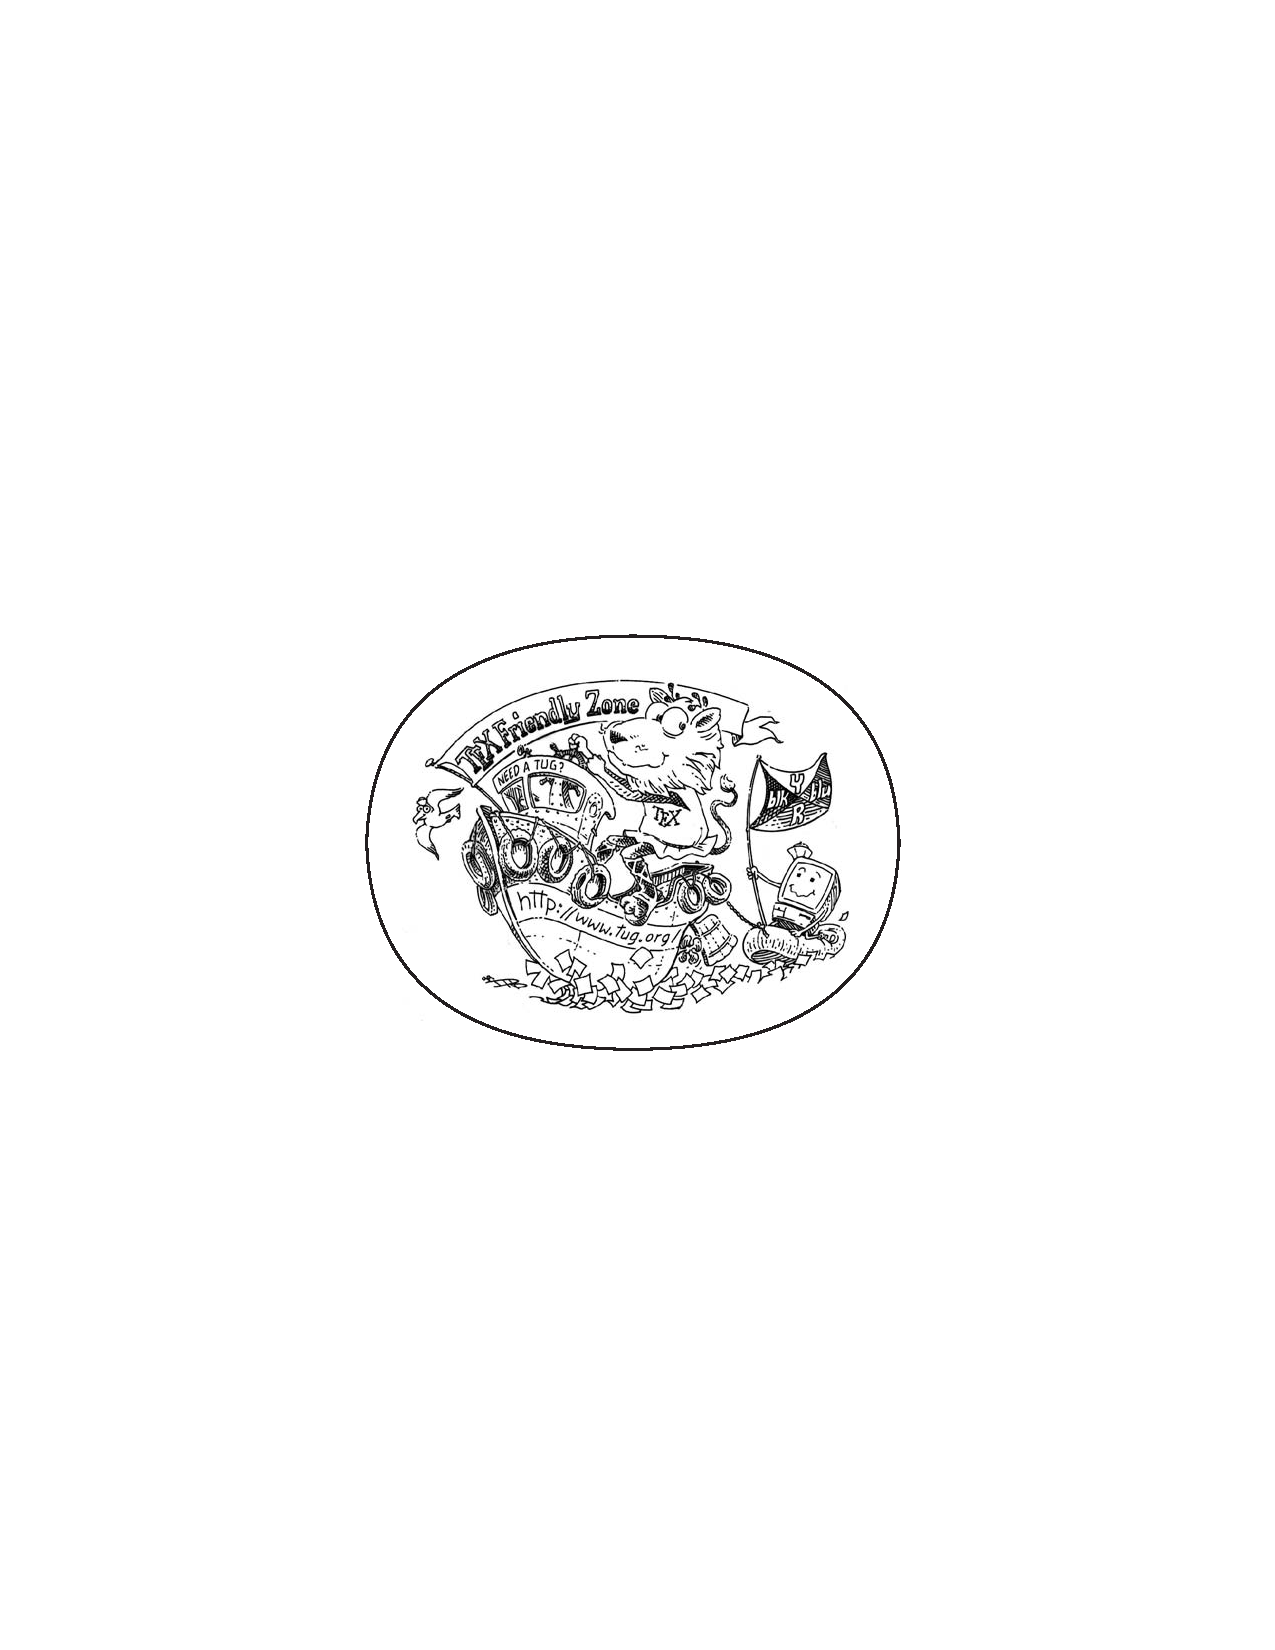
\includegraphics[width=6cm]{gfx/TFZsuperellipse_bw} \\ \medskip


		
\includegraphics[width=4cm]{gfx/logo_ugr}
	
        % \mySubtitle \\ \medskip
        %\myDegree \\
        %\myDepartment \\

        \vfill

        \myProf, \myOtherProf \\
        %\myFaculty \\
        \myUni \\ \bigskip

        \myTime\ %-- \myVersion

        %\vfill

    \end{center}
  \end{addmargin}
\end{titlepage}

    \thispagestyle{empty}

\hfill

\vfill

\noindent\myName: \textit{\myTitle,} \mySubtitle, %\myDegree, 
\textcopyright\ \myTime

%\bigskip
%
%\noindent\spacedlowsmallcaps{Supervisors}: \\
%\myProf \\
%\myOtherProf \\ 
%\mySupervisor
%
%\medskip
%
%\noindent\spacedlowsmallcaps{Location}: \\
%\myLocation
%
%\medskip
%
%\noindent\spacedlowsmallcaps{Time Frame}: \\
%\myTime

    \cleardoublepage%*******************************************************
% Dedication
%*******************************************************
\thispagestyle{empty}
%\phantomsection 
\refstepcounter{dummy}
\pdfbookmark[1]{Dedication}{Dedication}

\vspace*{3cm}

\begin{center}
    Ars est celare artem 
\end{center}


   %\cleardoublepage\include{FrontBackmatter/Foreword}
    \cleardoublepage%*******************************************************
% Abstract
%*******************************************************
%\renewcommand{\abstractname}{Abstract}
\pdfbookmark[1]{Abstract}{Abstract}
\begingroup
\let\clearpage\relax
\let\cleardoublepage\relax
\let\cleardoublepage\relax

\chapter*{Abstract}
General relativity theory predicts the existence of black holes, interesting objects that curve the spacetime in such a way that even the light cannot escape its attraction. The simulation of the trajectories followed by light near these bodies is of great interest for the scientific community, and this work serves this need.

As an introduction to general relativity theory from a basic mathematical background, this work studies the basic concepts and results needed in order to build a ray tracer that generates images of what an observer near a black hole would see.

The implemented code is parallelized using \ac{GPGPU} techniques, obtaining a software that is up to 125 times faster than the non-parallelized solutions.

The implemented code is distributed under a free software license in order to let the community download, use and contribute to the code without restrictions.

\vfill

\endgroup

\vfill

\textsc{\textbf{Keywords}}: black hole, differential geometry, ray tracer, general relativity, geodesics, graphics processing units, Kerr spacetime, semi-Riemannian geometry, parallelization.

   %\cleardoublepage%*******************************************************
% Publications
%*******************************************************
\pdfbookmark[1]{Publications}{publications}
\chapter*{Publications}\graffito{This is just an early --~and currently ugly~-- test!}
This might come in handy for PhD theses: some ideas and figures have appeared previously in the following publications:

%\noindent Put your publications from the thesis here. The packages \texttt{multibib} or \texttt{bibtopic} etc. can be used to handle multiple different bibliographies in your document.

\begin{refsection}[ownpubs]
    \small
    \nocite{*} % is local to to the enclosing refsection
    \printbibliography[heading=none]
\end{refsection}

\emph{Attention}: This requires a separate run of \texttt{bibtex} for your \texttt{refsection}, \eg, \texttt{ClassicThesis1-blx} for this file. You might also use \texttt{biber} as the backend for \texttt{biblatex}. See also \url{http://tex.stackexchange.com/questions/128196/problem-with-refsection}.
    \cleardoublepage%*******************************************************
% Acknowledgments
%*******************************************************
\pdfbookmark[1]{Acknowledgments}{acknowledgments}

\begin{flushright}{\slshape    
    We have seen that computer programming is an art, \\ 
    because it applies accumulated knowledge to the world, \\ 
    because it requires skill and ingenuity, and especially \\
    because it produces objects of beauty.} \\ \medskip
    --- \defcitealias{knuth:1974}{Donald E. Knuth}\citetalias{knuth:1974} \citep{knuth:1974}
\end{flushright}



\bigskip

\begingroup
\let\clearpage\relax
\let\cleardoublepage\relax
\let\cleardoublepage\relax
\chapter*{Acknowledgments}
Put your acknowledgments here.

Many thanks to everybody who already sent me a postcard!

Regarding the typography and other help, many thanks go to Marco 
Kuhlmann, Philipp Lehman, Lothar Schlesier, Jim Young, Lorenzo 
Pantieri and Enrico Gregorio\footnote{Members of GuIT (Gruppo 
Italiano Utilizzatori di \TeX\ e \LaTeX )}, J\"org Sommer, 
Joachim K\"ostler, Daniel Gottschlag, Denis Aydin, Paride 
Legovini, Steffen Prochnow, Nicolas Repp, Hinrich Harms, 
 Roland Winkler, Jörg Weber, Henri Menke, Claus Lahiri, 
 Clemens Niederberger, Stefano Bragaglia, Jörn Hees, 
 and the whole \LaTeX-community for support, ideas and 
 some great software.

\bigskip

\noindent\emph{Regarding \mLyX}: The \mLyX\ port was intially done by 
\emph{Nicholas Mariette} in March 2009 and continued by 
\emph{Ivo Pletikosi\'c} in 2011. Thank you very much for your 
work and for the contributions to the original style.


\endgroup




    \pagestyle{scrheadings}
    \cleardoublepage%*******************************************************
% Table of Contents
%*******************************************************
%\phantomsection
\refstepcounter{dummy}
\pdfbookmark[1]{\contentsname}{tableofcontents}
\setcounter{tocdepth}{2} % <-- 2 includes up to subsections in the ToC
\setcounter{secnumdepth}{3} % <-- 3 numbers up to subsubsections
\manualmark
\markboth{\spacedlowsmallcaps{\contentsname}}{\spacedlowsmallcaps{\contentsname}}
\tableofcontents 
\automark[section]{chapter}
\renewcommand{\chaptermark}[1]{\markboth{\spacedlowsmallcaps{#1}}{\spacedlowsmallcaps{#1}}}
\renewcommand{\sectionmark}[1]{\markright{\thesection\enspace\spacedlowsmallcaps{#1}}}
%*******************************************************
% List of Figures and of the Tables
%*******************************************************
\clearpage

\begingroup 
    \let\clearpage\relax
    \let\cleardoublepage\relax
    \let\cleardoublepage\relax
    %*******************************************************
    % List of Figures
    %*******************************************************    
    %\phantomsection 
    \refstepcounter{dummy}
    %\addcontentsline{toc}{chapter}{\listfigurename}
    \pdfbookmark[1]{\listfigurename}{lof}
    \listoffigures

    \vspace{8ex}

    %*******************************************************
    % List of Tables
    %*******************************************************
    %\phantomsection 
    \refstepcounter{dummy}
    %\addcontentsline{toc}{chapter}{\listtablename}
    \pdfbookmark[1]{\listtablename}{lot}
    \listoftables
        
    \vspace{8ex}
%   \newpage
    
    %%*******************************************************
    %% List of Listings
    %%*******************************************************      
    %  %\phantomsection 
    %\refstepcounter{dummy}
    %%\addcontentsline{toc}{chapter}{\lstlistlistingname}
    %\pdfbookmark[1]{\lstlistlistingname}{lol}
    %\lstlistoflistings 
    %
    %\vspace{8ex}
       
    %*******************************************************
    % Acronyms
    %*******************************************************
    %\phantomsection 
    \refstepcounter{dummy}
    \pdfbookmark[1]{Acronyms}{acronyms}
    \markboth{\spacedlowsmallcaps{Acronyms}}{\spacedlowsmallcaps{Acronyms}}
    \chapter*{Acronyms}
    \begin{acronym}[UMLX]
        \acro{DRY}{Don't Repeat Yourself}
        \acro{API}{Application Programming Interface}
        \acro{UML}{Unified Modeling Language}
        \acro{FIDO}{Fiducial Observer}
        \acro{ODE}{Ordinary Differential Equation}
        \acro{GPU}{Graphics Processing Unit}
        \acro{CPU}{Central Processing Unit}
        \acro{GPGPU}{General-Purpose Computing on Graphics Processing Units}
        \acro{SIMD}{Single Instruction Multiple Data}
        \acro{CUDA}{Compute Unified Device Architecture}
        \acro{API}{Application Programming Interface}
        \acro{BL}{Boyer-Lindquist}
    \end{acronym}                     
\endgroup


%********************************************************************
% Mainmatter
%*******************************************************
    \cleardoublepage\pagenumbering{arabic}
    %\setcounter{page}{90}
    % use \cleardoublepage here to avoid problems with pdfbookmark
    \cleardoublepage

    %\ctparttext{You can put some informational part preamble text here.
    %Illo principalmente su nos. Non message \emph{occidental} angloromanic
    %da. Debitas effortio simplificate sia se, auxiliar summarios da que,
    %se avantiate publicationes via. Pan in terra summarios, capital
    %interlingua se que. Al via multo esser specimen, campo responder que
    %da. Le usate medical addresses pro, europa origine sanctificate nos se.}

	% META-TODO: Clean the list of TODOs and remove this line :)
	\listoftodos[To do list]
	
	\part{Introduction}
	
    \part{Mathematics}
    \chapter{Lorentzian vector spaces}

This chapter follows the ideas on \cite{romero10}, which set up the basic background needed to understand what we will call later a spacetime, the main mathematical object in which we will develop our work.

Before going down that road we need to know what a Lorentzian vector space is and the basic concepts that we can build upon it.

\section{Basic definitions}

\begin{definition}[Lorentzian product and vector space]
	Let $V$ be an $n$-dimensional vector space on $\R$, with $n \geq 2$.
	
	A \emph{Lorentzian product on $V$} is a non-degenerate symmetric bilinear form on $V$ with index 1; that is, a bilinear form
	\[
		g \colon V \times V \to \R
	\]
	that satisfies the following:
	\begin{enumerate}
		\item $g$ is symmetric: $g(u, v) = g(v, u)$.
		\item $g$ is non-degenerate: if $g(u, v) = 0 \;\; \forall v \in V$, then $\Rightarrow u = 0$.
		\item $g$ has index 1: the maximum dimension of a subspace $W$ in which $g(u,u) \leq 0 \; \forall u \in W$ ---where equality holds if and only if $u = 0$--- is 1.
	\end{enumerate}

	The vector space $V$ furnished with such a Lorentzian product is called a \emph{Lorentzian vector space}.
\end{definition}

As usual, we will say that two vectors are \emph{orthogonal} on $(V,g)$ whenever $g(u,v) = 0$.

From now on until the end of this chapter, let us consider $(V,g)$ a Lorentzian vector space.

When such a Lorentzian product is added to a vector space, its elements can be classified depending on the value of the metric on them.

\begin{definition}[Classification of vectors on Lorentzian vector spaces]
	A vector $v \in V$ is said to be:
	\begin{itemize}
		\item \emph{spacelike} if $g(v,v) > 0$ or $v = 0$,
		\item \emph{timelike} if $g(v,v) < 0$ or
		\item \emph{null} or \emph{lighlike} if $g(v,v) = 0$ with $v \neq 0$.
	\end{itemize}
\end{definition}

\begin{definition}[Light cone]
	The \emph{light cone of $V$} is the subset of all null vectors.
\end{definition}

The study of the Lorentzian vector spaces will be based on \autoref{lem:lorentzspan}, which classifies, for each timelike vector, all elements of $(V,g)$ on two orthogonal subsets.

\begin{lemma}
	\label{lem:lorentzspan}
	Let $v \in V$ be a timelike vector. Then, we can split the vector space as follows:
	\[
		V = \langle v \rangle \oplus v^\perp,
	\]
	where $v^\perp \defeq \{u \in V / g(u,v) = 0\} = \langle v \rangle^\perp$.
	
	Furthermore, $g_{\mid_{v^\perp}}$ is positive definite and $g_{\mid_{\langle v \rangle}}$ is negative definite; \ie, $g_{\mid_{v^\perp}}$ and $-g_{\mid_{\langle v \rangle}}$ are Euclidean products.
\end{lemma}

\begin{proof}
	As $\langle v \rangle$ is non degenerate, so it is $v^\perp$. Then, $V = \langle v \rangle + v^\perp$ is a direct sum. As the $v^\perp$ index is necessarily zero, $v^\perp$ is spacelike and, consequently
	
	See \cite[Lemma 5.26]{oneill83} for details.
\end{proof}

\begin{remark}\label{classic_Schwarz}
	The positive definite subspaces of a Lorentzian vector space are in fact Euclidean spaces; in particular, the Schwarz inequality holds in $v^\perp$, with $v$ a timelike vector:
    \begin{equation}
	    \label{eq:schwarz}
        \lvert g(u,w) \rvert \leq \sqrt{g(u,u)} \sqrt{g(w,w)} \quad \forall u,w \in v^\perp,
    \end{equation}
    with equality if and only if $u$ and $w$ are linearly dependent.
\end{remark}

Then, it is trivial that two timelike vectors are never orthogonal. An interesting result appears when we study what happens with two orthogonal null vectors.

From \cite[Cor. 1.1.5]{sachs77}, \cite[p. 155]{oneill83}, we can see:

\begin{proposition} Let $x,y \in V$ be two null vectors. Then
	\[
		$g(x,y)=0$ \Leftrightarrow $x$ \textrm{ and } $y$ \textrm{ are linearly dependent}.
	\]
\end{proposition}

\begin{proof}
    From \autoref{lem:lorentzspan} we can write $V=\langle v \rangle \oplus v^{\perp},$ with $g(v,v)=-1$. Therefore, there exist $a,b \in \R\setminus\{0\}$ and $u,w \in v^\perp$ such that:
    \begin{align*}
        x=av+u, \quad u\neq 0, \quad g(u,u)=a^2,\\
        y=bv+w, \quad w\neq 0, \quad g(v,v)=b^2.
    \end{align*}
    If $g(x,y)=0$ then $\lvert g(u,w) \rvert = \sqrt{g(u,u)}\sqrt{g(w,w)}$ and therefore, from \autoref{eq:schwarz}, $u=kw$ for some $k\in \R$. In fact, $k=a/b$. The converse is trivial.
\end{proof}

\section{Time cones}

From now on, $\mathcal{T}(V,g)$ will denote the set of all timelike vectors on $(V,g)$.

\begin{definition}[Time cone]
	Let $v\in \mathcal{T}(V,g)$ be a timelike vector. The \emph{time cone defined by $v$} is the set
	\[
	C(v)=\{u\in\mathcal{T}(V,g)\, : \, g(u,v)<0 \}.
	\]
\end{definition}

It is clear that $C(v)$ is not empty, as $v$ itself lays on its own time cone.

Furthermore, as no two timelike vector can be orthogonal, $g(v,w) \neq 0$ for each $w \in \mathcal{T}(V,g)$; \ie, either $w\in C(v)$ or $w\in C(-v)$. This let us describe $\mathcal{T}(V,g)$ as a union of two time cones for each timelike vector.
\[
\mathcal{T}(V,g) = C(v) \cup C(-v) \quad \forall v\in \mathcal{T}(V,g)
\]

The following result characterizes when two timelike vectors lie in the same time cone 

It is interesting to know when two timelike vectors lie in the same time cone. \autoref{lem:timecone}, based on \cite[Lemma 5.29]{oneill83}, gives us the answer.

\begin{lemma}\label{lem:timecone}
Given $u,v\in \mathcal{T}(V,g)$, they belong to the same time cone if and only if $g(u,v)<0$.
\end{lemma}

\begin{proof}
    By definition, if $g(u,v)<0$, then $u\in C(v)$, and therefore $u$ and $v$ belong to the time cone defined by $v$.
    
    Assume now that $u$ and $v$ belong to a same time cone defined by a $w \in V$ such that $g(w,w) = -1$. Using \autoref{lem:lorentzspan} we can write
    \begin{align*}
        u=aw+y, \quad y\in w^{\perp}, \quad a=-g(u,w)>0,\\
        v=bw+z, \quad z\in w^{\perp}, \quad b=-g(v,w)>0.
    \end{align*}
    Taking into account
    \[
	    \sqrt{g(y,y)}<a \quad \mathrm{and} \quad \sqrt{g(z,z)}<b,
    \]
    we have
    \[
	    g(u,v)\leq -ab+ \lvert g(y,z) \rvert \leq -ab + \sqrt{g(y,y)}\sqrt{g(z,z)}<-ab+ab=0.
    \]
\end{proof}

\begin{corollary}\label{convexity}
Let $w\in\mathcal{T}(V,g)$, $u,v\in C(w)$ and $a,b\in \R$ with $a,b\geq 0$ and $a^2+b^2 \neq 0$. Then, we have $au+bv\in C(w)$.
\end{corollary}

\begin{proof}
    As $g(au+bv,w)=a g(u,w)+ b g(v,w)<0$, \autoref{lem:timecone} proves the result.
\end{proof}

This corollary let us conclude that time cones are convex subsets of $V$. Furthermore, it is important to realize that if $u\in C(v)$ then $C(u)=C(v)$.

\autoref{classic_Schwarz} showed that the Schwarz inequality holds on the orthogonal space of any timelike vector. This result is not true if we consider any pair of vectors, but what happens when we focus on timelike vectors? Some interesting results will appear.

\section{Wrong-way inequalities}

First of all, we can obtain an the so-called \emph{wrong-way Schwarz inequality} ---see \cite[Prop. 5.30]{oneill83}--- when considering only timelike vectors.

\begin{proposition}[Wrong-way Schwarz inequality]
	\label{pro:wrongway}
    Let $u,v \in \mathcal{T}(V,g)$ be a pair of timelike vectors. Then, its product satisfies the following:
    \[
        \lvert g(u,v) \vert \geq \sqrt{-g(u,u)}\sqrt{-g(v,v)}
    \]
    with equality holding if and only if $u$ and $v$ are linearly dependent.
\end{proposition}

\begin{proof}
    Using \autoref{lem:lorentzspan}, we know there exists $a \in \R$ and $x \in v^\perp$ such that $u=av+x$, and therefore
    \[
        g(u,v)^2=a^2g(v,v)^2, \quad \quad g(u,u)=a^2g(v,v)+g(x,x)<0,
    \]
    which gives
    \[
        g(u,v)^2=\{g(u,u)-g(x,x)\}g(v,v) \geq g(u,u)g(v,v).
    \]
    The equality holds if and only if $g(x,x)=0$, \ie, if and only if $x=0$, which means $u=av$.
\end{proof}


We can obtain another wrong-way inequality. As a consequence of \autoref{pro:wrongway} and using \autoref{lem:timecone}, the so-called \emph{wrong-way Minkowski inequality} is found ---see \cite[Cor. 5.31]{oneill83}---.

\begin{corollary}[Wrong-way Minkowski inequality]
	\label{Minkowski}
    Let $u,v \in \mathcal{T}(V,g)$ be two timelike vector that lie in the same time cone. The following inequality is hold:
    \[
        \sqrt{-g(u+v,u+v)} \geq \sqrt{-g(u,u)}+\sqrt{-g(v,v)}
    \]
    and equality holds if and only if $u$ and $v$ are linearly dependent.
\end{corollary}

We can now formalize the notion of angle between two timelike vectors.

Indeed, let $u, v \in \mathcal{T}(V,g)$ be two timelike vectors that lie in the same time cone. From \autoref{lem:timecone} and \autoref{pro:wrongway}, we know that
\[
-g(u,v) \geq \sqrt{-g(u,u)}\sqrt{-g(v,v)},
\]
and therefore, there exists a unique $\theta \in \R$, $\theta \geq 0$, such that
\[
\cosh \theta =\frac{-g(u,v)}{\sqrt{-g(u,u)}\sqrt{-g(v,v)}}.
\]

$\theta$ is called the \emph{hyperbolic angle} between $u$ and $v$.

\section{Time orientation}

This last section on Lorentzian vector spaces introduces an important concept: the time orientation. We need some previous concepts before formalizing this idea.

\begin{definition}[Orthonormal basis of $(V,g)$]
	Let $B = (v_1, \dots, v_n)$ be a basis of $V$. $B$ is said to be \emph{orthonormal} when
	\begin{itemize}
		\item any two different vectors on $B$ are $g$-orthogonal,
		\item each $v_i$, with $i \in \{1,\dots,n-1\}$, is unitary spacelike and
		\item $v_n$ is unitary timelike.
	\end{itemize}

	Note that the matrix of $g$ on the basis $B$ is
	\[
		M_B(g) = \begin{pmatrix}
			I_{n-1} & 0  \\
			0 & -1
		\end{pmatrix}.
	\]
\end{definition}

Let $B = (v_1, \dots, v_n)$ and $B' = (v'_1, \dots, v'_n)$ be two orthonormal basis of $(V,g)$. We say that $B$ and $B'$ define the same \emph{time orientation} of $(V,g)$ when
\[
	g(v_n, v'_n) < 0;
\]
that is, when both $v_n$ and $v'_n$ lie in the same time cone of $(V,g)$.

This defines two equivalence classes on the set of orthonormal basis: the class defined by $B=(v_1,..,v_{n-1},v_n)$ and the class defined by $\tilde{B}=(v_1,..,v_{n-1},-v_n)$.

\begin{definition}[Time orientation]
	A \emph{time orientation} on $(V,g)$ is each one of the two equivalence classes defined by $B$ and $\tilde{B}$.
\end{definition}

Furthermore, we note that a time orientation on $(V,g)$ is given by each time cone of $(V,g)$.

Although the classical orientations on $V$ does not depend on $g$, it is important to realize that the notion of time orientation is a metric concept, that is, it is defined using the Lorentzian product $g$.

However, a time orientation does not change if we replace $g$ by a conformally related Lorentzian product $ag$, with $a\in \R$, $a>0$.

\section{Topological remarks}

We end this section explaining some topological remarks. If $V$ is an $n$-dimensional vector space and $B$ is a basis of $V$, then we have a linear isomorphism $$b_B : V \longrightarrow \R^n,$$ defined by $b_B(v)=(a_1,..,a_n)$, where $(a_1,..,a_n)$ are the coordinates of $v$ in $B$. By using $b_B$ a topology $\mathfrak{T}_B$ can be defined in $V$ in such a way that the $\mathfrak{T}_B$-open subsets of $V$ are $b_B^{-1}(O)$, where $O$ is an open subset of $\R^n$. It is not difficult to see that $\mathfrak{T}_B = \mathfrak{T}_{B'}$ for any basis $B,B'$ of $V$. Endowed with this topology, the function $V \longrightarrow \R$, given by $v \mapsto g(v,v)$ is continuous. Hence $\mathcal{T}(V,g)$ is an open subset of $V$ and each time cone is also an open subset of $V$. Moreover, the set of nonzero spacelike vectors $\{v\in V \, : \, g(v,v)>0 \}$ is an open subset of $V$ and the light cone with the zero vector $\{v\in V \, : \, g(v,v)=0 \}$ is a closed subset of $V$. Finally, every null vector can be obtained as the limit of a sequence of timelike vectors as well of spacelike vectors (or both types of vectors). Thus, $\{v\in V \, : \, g(v,v)<0 \} \cup \{v\in V \, : \, g(v,v)>0 \}$
is a dense subset of $V$.

    \chapter{Tensor Algebra}\fixme{Add references throughout the text.}

This chapter covers some basic tools needed in the further development of this work. Although basic, its knowledge is crucial on a lot fields, and its interest for the study of the Geometry will unveil on the following chapters.

Nearly all definitions, results and ideas are based on \cite[Chapters 6 and 9]{romero86}.

\section{The notion of tensor}

\begin{definition}[Multilinear map]
	\label{def:multilinear}
    Let $V_1, V_2, \dots, V_r$ and $W$ be vector spaces over the same field $K$. A multilinear ---$r$ times linear--- map from $V_1 \times V_2 \cdots \times V_r$ to $W$ is a map
    \[
        T \colon V_1 \times V_2 \cdots \times V_r \longrightarrow W
    \]
    that is linear in each of its components; \ie, that verifies the following conditions:
    \begin{enumerate}
        \item $\begin{aligned}[t]
	        T(x_1, \dots, x_i+x_i', \dots, x_r) = &T(x_1, \dots, x_i, \dots, x_r) + \\&T(x_1, \dots, x_i', \dots, x_r),
        \end{aligned}$
        \item $T(x_1, \dots, a x_i, \dots, x_r) = aT(x_1, \dots, x_i, \dots, x_r)$,
    \end{enumerate}
    for every $i \in \{1, 2, \dots, r\}$, where $x_j$ is an arbitrary vector in $V_j$ and $a \in K$.
\end{definition}

Before going ahead with the definition of tensor, we must remember the concept of dual space.

Given a vector space $V$ over a field $K$, its \emph{dual space} is the vector space defined as
\[
	V^* \defeq \Hom_K(V,K);
\]
that is, $V^*$ is the set of all linear maps $\varphi : V \to K$.

There are some interesting results concerning dual spaces that will be important in the understanding of the notion of tensor.

First of all, it is known that if $V$ is finite-dimensional, the dimensions of $V$ and $V^*$ are the same and, given a base of $V$, $B = \{v_1, \dots, v_n\}$, its \emph{dual basis} is built as $B^* = \{\varphi^1, \dots, \varphi^n\}$\footnote{From now on, Latin letters with subscripts will denote vectors, whereas Greek letters with superscripts will denote one-forms.}, where
\[
	\varphi^i(v_j) = \delta^i_j.
\]

Furthermore, the reflexiveness theorem \change{Reflexiveness theorem is the worst translation ever} tells us that there exists a natural isomorphism between $V$ and its double dual space, $V^{**}$, when $V$ is finite-dimensional. This isomorphism assigns, to every vector $v \in V$, a function that maps every one-form into its evaluation on $v$:
\begin{align}
	\label{eq:naturaliso}
	\psi \colon V &\longrightarrow V^{**} \\
	v &\longmapsto \psi_v \colon \begin{aligned}[t]
		V^* &\longrightarrow K \\
		\varphi &\longmapsto \varphi(v).
	\end{aligned} \nonumber
\end{align}

With the concepts of multilinear maps and dual spaces we can now build the definition of tensor, core concept of this section.

\begin{definition}[Tensor]
	\label{def:tensor}
	Let $V$ be a vector space over a field $K$, being $V^*$ its dual space. A tensor $r$ ($\geq 0$) times contravariant and $s$ ($\geq 0$) times covariant ---\ie, a tensor of type $(r,s)$--- is a multilinear map
	\[
		T \colon \underbrace{V^* \times \cdots \times V^*}_{\text{r copies}} \times \underbrace{V \times \cdots \times V}_{\text{s copies}} \longrightarrow K.
	\]
	Tensors of type $(0,s)$ are said to be \emph{covariant}, whereas tensors of type $(r,0)$ are called \emph{contravariant}.

	The \emph{order} of the tensor is defined as the sum $r+s$.
\end{definition}

\begin{example}
	\label{ex:tensors}
	The following examples show how interesting the notion of tensor is, as it can include a vast selection of mathematical objects under the same concept; for example, we will see that both vectors and one-forms are tensors.

	Let $V$ be an $n$-dimensional vector space and $V^*$ its dual space.
	\begin{enumerate}
		\item Let $\varphi \in V^*$; \ie,  $\varphi \colon V \to K$ is a one-form. From \autoref{def:tensor} it is clear that $\varphi$ is a tensor of type $(0,1)$ over $V$.
		\item Let $v \in V$ be a vector. Using the natural isomorphism between $V$ and its double dual space, the vector $v$ can be identified with $\psi_v \colon V^* \to K$, and thus we can understand $v$ as a tensor of type $(1,0)$.
		\item Consider now $f \in \End_K V$ and let $T_f \colon V^* \times V \to K$ be the map defined as $T_f(\varphi, v) \defeq \varphi(f(v))$. It is clear that $T_f$ is a tensor of type $(1,1)$. Moreover, if we consider $f$ to be the identity map $1_V$, then $T_{1_V}$ is the tensor that maps every pair of (vector, one-form) to the evaluation of the one-form on the vector; \ie, is the tensor associated to the natural isomorphism between $V$ and $V^{**}$.
		\item Common operations on several mathematical fields can also be seen as tensors. For example, the inner product can be defined as a tensor of type $(0,2)$ as follows:
		\begin{align*}
			T \colon V \times V &\to K\\
			(v,w) &\mapsto \sum_{i=1}^n v_i w_i.
		\end{align*}
		In general, every bilinear form is a $(0,2)$ tensor. This follows from the definition of bilinear form, which satisfies all conditions in \autoref{def:tensor}.
	\end{enumerate}
\end{example}

\section{Tensor addition, product by a scalar and tensor product}
Let $\tensors_{r,s}(V)$ be the set of all tensors of type $(r,s)$. It is clear that both $\tensors_{1,0}(V) = V^*$ and $\tensors_{0,1}(V) = V^{**}$ are vector spaces over K. A natural question arises: is $\tensors_{r,s(V)}$ a vector space for arbitrary $r$ and $s$? The following result gives us the answer we are looking for.

\begin{theorem}
	Let $T, T' \in \tensors_{r,s}(V)$ be two tensors of type $(r,s)$ and $a \in K$ a scalar. Consider the following operations:
	\begin{itemize}
		\item $\begin{aligned}[t]
			(T+T') (\varphi^1, \dots, \varphi^r, v_1, \dots, v_s) \defeq &T(\varphi^1, \dots, \varphi^r, v_1, \dots, v_s) +\\
			&T'(\varphi^1, \dots, \varphi^r, v_1, \dots, v_s),
		\end{aligned}$
		\item $(a T)(\varphi^1, \dots, \varphi^r, v_1, \dots, v_s) \defeq a T(\varphi^1, \dots, \varphi^r, v_1, \dots, v_s)$,
	\end{itemize}
	where $\varphi^i \in V^*$ for all $i \in \{1,\dots,r\}$ and $v_j \in V$ for all $j \in \{1,\dots,s\}$.

	The set $\tensors_{r,s}(V)$ with the preceding operations is a vector space.
\end{theorem}

\begin{proof}
	It is clear, from \autoref{def:tensor}, that $T+T', aT \in \tensors_{r,s}(V)$, given the linearity in each of the components of both $T$ and $T'$.
	These operations satisfy the following properties:
	\begin{enumerate}
		\item $(T+T') + T'' = T + (T'+T'')$.
		\item There exists a \emph{null tensor} $T_0 \in \tensors_{r,s}(V)$, defined as \[T_0(\varphi^1, \dots, \varphi^r, v_1, \dots, v_s) = 0, \forall \varphi^i \in V^*, \forall v_i \in V,\] such that $T_0 + T = T + T_0 = T \;\forall T \in \tensors_{r,s}(V)$.
		\item For each $T\in\tensors_{r,s}(V)$ there exists an \emph{opposite tensor} $-T$ defined as \[(-T)(\varphi^1, \dots, \varphi^r, v_1, \dots, v_s) = - T(\varphi^1, \dots, \varphi^r, v_1, \dots, v_s)\] that satisfies $T + (-T) = -T + T = 0$.
		\item $T + T' = T' + T$.
	\end{enumerate}
	This provides abelian goup structure to $\tensors_{r,s}(V)$. The following properties finally show that $\tensors_{r,s}(V)$ is a vector space:
	\begin{enumerate}
		\item $a(T+T') = aT+ aT', \;\;\forall a \in K, \;\forall T,T' \in \tensors_{r,s}(V)$.
		\item $(a+b)T = aT + bT, \;\;\forall a,b \in K, \;\forall T \in \tensors_{r,s}(V)$.
		\item $(ab)T = a(bT), \;\;\forall a,b \in K, \;\forall T \in \tensors_{r,s}(V)$.
		\item $1T = T, \;\;\forall T \in \tensors_{r,s}(V)$, where $1$ is the unity in $K$.
	\end{enumerate}
\end{proof}

Now that we know that $\tensors_{r,s}(V)$ is a vector space, it will be important to study its dimension. Before going down that road, let us define the tensor product, concept upon which we will be able to build a basis for $\tensors_{r,s}(V)$.

\begin{definition}[Tensor product]
	Let $T \in \tensors_{r,s}(V)$ and $T' \in \tensors_{r',s'}(V)$. The \emph{tensor product} \[T \otimes T' \colon \underbrace{V^* \times \cdots \times V^*}_{\text{r+r' copies}} \times \underbrace{V \times \cdots \times V}_{\text{s+s' copies}}\] is defined as follows:
	\begin{align*}
		&(T \otimes T')(\varphi^1, \dots, \varphi^{r+r'}, v_1, \dots, v_{s+s'}) \defeq \\
		&T(\varphi^1, \dots, \varphi^r, v_1, \dots, v_s) T(\varphi^{r+1}, \dots, \varphi^{r+r'}, v_{s+1}, \dots, v_{s+s'}),
	\end{align*}
	where $\varphi^i \in V^*$ for all $i \in \{1,\dots,r+r'\}$ and $v_j \in V$ for all $j \in \{1,\dots,s+s'\}$.
\end{definition}

It is easy to prove that $T \otimes T' \in \tensors_{r+r',s+s'}(V)$ for every $T \in \tensors_{r,s}(V)$ and $T' \in \tensors_{r',s'}(V)$. However, the proof is long and cumbersome to write, and it can be found in almost every elementary book on tensor algebra.\unsure{Add reference.}

Furthermore, we can see that, given $T \in \tensors_{r,s}(V)$, $T' \in \tensors_{r',s'}(V)$ and $T'' \in \tensors_{r'',s''}(V)$:
\begin{align*}
	(T \otimes T') \otimes T'' &\in \tensors_{r+r'+r'', s+s'+s''}(V),\\
	T \otimes (T' \otimes T'') &\in \tensors_{r+r'+r'', s+s'+s''}(V)
\end{align*}
and that the following equality holds:
\[
	(T \otimes T') \otimes T'' = T \otimes (T' \otimes T'').
\]
In fact, the application
\begin{align*}
	\tensors_{r,s}(V) \times \tensors_{r',s'}(V) &\longrightarrow \tensors_{r+r',s+s'}(V) \\
	(T,T') &\longmapsto T \otimes T'
\end{align*}
is a bilinear map.

As a particular example, we can define the tensor product between two tensors of type $(1,0)$ and $(0,1)$ as the following tensor:\footnote{Note that we are using the reflexiveness theorem to ease the notation, as we are writing $v$ ---a letter used for vectors of $V$--- to describe an element of $V^{**}$.}
\[
	v \otimes \varphi \in \tensors_{1,1}(V),
\]
which maps every pair $(\psi, w)$ to the scalar $\psi(v)\varphi(w)$.

Upon this concept, and using the known properties of the dual vector space and its basis, we can state and prove a theorem that builds a basis for every $\tensors_{r,s}(V)$.

\begin{theorem}
	Let $V$ be an $n$-dimensional vector space over a field $K$. Let $\mathcal{B} = \{v_1, \dots, v_n\}$ be a basis of $V$ and $\mathcal{B^*} = \{\varphi^1, \dots, \varphi^n\}$ be  its dual basis. Then,
	\begin{align*}
		\mathcal{B}_T = \{v_{i_1} \otimes \dots \otimes v_{i_r} \otimes \varphi^{j_1} \otimes \dots \otimes \varphi^{j_s} \textrm{ , } &\textrm{where every index moves} \\
		&\textrm{independently from $1$ to $n$}\},
	\end{align*}
	is a basis of $\tensors_{r,s}(V)$. As a consequence, $\dim_K\tensors_{r,s}(V) = n^{r+s}$.
\end{theorem}

\begin{proof}
	%First of all, let us note $t^{i_1,\dots,i_r}_{j_1,\dots,j_s} \defeq T(\varphi^{i_1}, \dots, \varphi^{i_r}, v_{j_1}, \dots, v_{j_r}) \in K$.

	In order to prove that $\mathcal{B}_T$ is a linear span of $\tensors_{r,s}(V)$, let us consider $T\in\tensors_{r,s}(V)$. Then, if
	\begin{align*}
		\psi^1& = \sum_{i_1 = 1}^n a_{i_1}^1 \varphi^{i_1},\quad \cdots,\quad \psi^r = \sum_{i_r = 1}^n a_{i_r}^r \varphi^{i_r} \textrm{ and} \\
		w_1 &= \sum_{j_1 = 1}^n b^{j_1}_1 v_{j_1},\quad \cdots,\quad w_s = \sum_{j_s = 1}^n b^{j_s}_s v_{j_s},
	\end{align*}
	we can write
	\[
		T(\psi^1, \dots, \psi^r, w_1, \dots, w_s) = \sum_{\substack{i_1,\dots,i_s\\j_1,\dots,j_r}} a_{i_1}^1 \cdots a_{i_r}^r b^{j_1}_1 \dots b^{j_s}_s t_{j_1, \dots, j_s}^{i_1, \dots, i_r},
	\]
	where $t_{j_1, \dots, j_s}^{i_1, \dots, i_r} \defeq T(\varphi^{i_1}, \dots, \varphi^{i_r}, v_{j_1}, \dots, v_{j_s})$.

	Following this reasoning ---see \cite{romero86} for the details---, we can finally write
	\[
		T = \sum_{\substack{i_1,\dots,i_s\\j_1,\dots,j_r}} t_{j_1, \dots, j_s}^{i_1, \dots, i_r} \left( v_{i_1} \otimes \dots \otimes v_{i_r} \otimes \varphi^{j_1} \otimes \dots \otimes \varphi^{j_s} \right),
	\]
	which proves that $\mathcal{B}_T$ spans $\tensors_{r,s}(V)$.

	To prove that $\mathcal{B}_T$ is linearly independent, consider a linear combination of the elements in $\mathcal{B}_T$ that equals the null tensor,
	\begin{equation}
		\label{eq:nullcomb}
		\sum_{\substack{k_1,\dots,k_r\\l_1,\dots,l_s}} a^{k_1,\dots,k_r}_{l_1,\dots,l_s} \left( v_{k_1} \otimes \dots \otimes v_{k_r} \otimes \varphi^{l_1} \otimes \dots \otimes \varphi^{l_s} \right) = T_0
	\end{equation}
	Evaluating both sides of \autoref{eq:nullcomb} on the corresponding elements of the bases $\mathcal{B}$ and $\mathcal{B}^*$ we obtain the equality
	\[
		\sum_{\substack{k_1,\dots,k_r\\l_1,\dots,l_s}} a^{k_1,\dots,k_r}_{l_1,\dots,l_s} \left( \delta^{i_1}_{k_1} \dots \delta^{i_r}_{k_r} \delta^{l_1}_{j_1} \dots \delta^{l_s}_{j_s} \right) = 0,
	\]
	from which it is clear that $a^{i_1,\dots,i_r}_{j_1,\dots,j_s} = 0$ for every index.
\end{proof}

Two particularly important examples of the above theorem let us grasp the duality between vectors and one-forms.

Let $V$ be a vector space with dimension $n$, with basis $B = \{v_1, \dots, v_n\}$ and dual basis $B^* = \{\varphi^i, \dots, \varphi^n\}$.

We know that $\tensors_{1,0}(V) = V^{**}$, and using reflexiveness theorem we can write each vector $v \in V \simeq V^{**}$ as
\[
v = \sum_{i=1}^n b^i v_i,
\]
where each coordinate is the projection of the vector using the corresponding one-form: $b^i = \varphi^i(v)$.

Similarly, we can consider $\tensors_{0,1}(V) = V^*$. Each of its elements, $\psi \in V^*$, can be written in terms of the tensor basis $\mathcal{B}_{\tensors_{0,1}(V)} = B^*$:
\[
	\psi = \sum_{j=1}^n a_j \varphi^j,
\]
Note here that the coordinates are retrieved evaluating the form in each element of the basis $B$: $a_j = \psi(v_j)$.

This shows that both evaluating a one-form on the elements of the basis $B$ and projecting a vector with the elements of the basis $B^*$ can be seen as dual operations: both of them gives the coordinates of the corresponding element on the corresponding basis.

The notion of tensor help us to understand this duality: we now see both elements as the \emph{same} mathematical entity, where both operations are expressed in different bases with the corresponding change of coordinates.

\section{Change of bases on $\tensors_{r,s}(V)$}

We now want to study how the coordinates of a tensor change when we change the basis of $\tensors_{r,s}(V)$.

First of all, we must remember the relationship between the change of basis on a vector space $V$ and the corresponding change of basis in its dual space, $V^*$.

Let $B = (v_1, \dots, v_n)$ and $B' = (v_1', \dots, v_n')$ be two bases of $V(K)$, and suppose that the change of coordinates is given by
\[
v_j = \sum_{i=1}^n a_j^i v'_i.
\]

It is known that ---see \cite[p. 162]{romero86}---, if $B^* = (\varphi^1, \dots, \varphi^n)$ and $B'^* = (\varphi'^1, \dots, \varphi'^n)$ are the dual bases of the two preceding ones, the elements of the bases are related in the \emph{opposite} way as before:
\begin{equation}
	\label{eq:changeV*}
	\varphi'^i = \sum_{j=1}^n a_j^i \varphi^j \textrm{, where } a_j^i \in K.
\end{equation}

Furthermore, we can see that
\begin{equation}
	\label{eq:changeV}
	v_j' = \sum_{j=1}^n b_j^i v_j,
\end{equation}

where $b_j^i$ is the element placed on the $i$-th row, $j$-th column of  the inverse matrix of $(a^i_j)$.

This change of bases in $V$ and $V^*$  is key to understand \autoref{pro:changeT}, which tells us how  the coordinates of a tensor change when we change the basis of $\tensors_{r,s}(V)$.

\begin{proposition}
	\label{pro:changeT}
	Let $B$, $B'$ and $B^*$, $B'^*$ the bases of $V$ and $V^*$ described above and consider two ordered bases of $\tensors_{r,s}(V)$ obtained from
	\begin{align*}
		\mathcal{B}_T = \{v_{i_1} \otimes \dots \otimes v_{i_r} \otimes \varphi^{j_1} \otimes \dots \otimes \varphi^{j_s} \textrm{ , } &\textrm{where every index moves} \\
		&\textrm{independently from $1$ to $n$}  \}
	\end{align*}
	and
	\begin{align*}
		\mathcal{B}'_T = \{v'_{i_1} \otimes \dots \otimes v'_{i_r} \otimes \varphi'^{j_1} \otimes \dots \otimes \varphi'^{j_s} \textrm{ , } &\textrm{where every index moves} \\
		&\textrm{independently from $1$ to $n$}  \}.
	\end{align*}

	Then, the analytic expression of the change of coordinates of a tensor $T \in \tensors_{r,s}(V)$ is the following:
	\begin{align*}
		t'^{k_1,\dots,k_r}_{\phantom{'}l_1,\dots,l_s} = \sum a_{i_1}^{k_1} \cdots a_{i_k}^{k_r} b_{l_1}^{j_1} \cdots b_{l_s}^{j_s} t_{j_1,\dots,j_s}^{i_1,\dots,i_r}
	\end{align*}
	where the coefficients are the ones defined in \autoref{eq:changeV*} and \autoref{eq:changeV}.
\end{proposition}

\begin{proof}
	Considering the change of bases in $V$ and $V^*$, the proof is direct, using the definition of the coordinates of a tensor $T \in \tensors_{r,s}(V)$:
	\begin{align*}
		t'^{k_1,\dots,k_r}_{\phantom{'}l_1,\dots,l_s} &= T(\varphi'^{k_1}, \dots, \varphi'^{k_r}, v_{l_1}', \dots, v_{l_s}')  = \\
		&= T(\sum a_{i_1}^{k_1}\varphi^{i_1}, \dots, \sum a_{i_r}^{k_r}\varphi{i_r}, \sum b_{l_1}^{j_1} v_{j_1}, \dots, \sum b_{l_s}^{j_s} v_{j_s}) = \\
		&= \sum a_{i_1}^{k_1} \cdots a_{i_k}^{k_r} b_{l_1}^{j_1} \cdots b_{l_s}^{j_s} T(\varphi^{k_1}, \dots, \varphi^{k_r}, v_{l_1}, \dots, v_{l_s}) = \\
		&= \sum a_{i_1}^{k_1} \cdots a_{i_k}^{k_r} b_{l_1}^{j_1} \cdots b_{l_s}^{j_s} t_{j_1,\dots,j_s}^{i_1,\dots,i_r}
	\end{align*}
\end{proof}

\subsection*{Tensors of order 2}
\label{sub:order2}

We can study now the particular examples of tensors of order 2. From now on, let $V$ be an $n$-dimensional vector space, $V^*$ its dual space and $\mathcal{B} = (v_1, \dots, v_n)$ and $\mathcal{B^*} = (\varphi^1, \dots, \varphi^n)$ their respective bases.

Let us first consider $\tensors_{(2,0)}$, which is a vector space of dimension $n^2$. Let
\[
	\mathcal{B}_T = \{v_i \otimes v_j \textrm{, where } i,j \in \{1,\dots,n\}\}
\]
be one of its bases. We can now write a generic tensor $T\in\tensors_{2,0}$ as follows:
\[
	T = \sum_{i,j=1}^n t^{ij} v_i \otimes v_j,
\]
where $t^{ij} = T(\varphi^i, \varphi^j)$.

Let $\mathcal{B}' = (v_1', \dots, v_n')$ and $\mathcal{B}'^* = (\varphi'^1, \dots, \varphi'^n)$ be two new bases of $V$ and $V^*$.

Following \autoref{pro:changeT}, we know that $T = \sum_{i,j=1}^n t^{ij} v_i \otimes v_j = \sum_{k,l=1}^n t'^{kl} v_k' \otimes v_l'$, where
\[
	t'^{kl} = \sum_{i,j=1}^n a^k_i a^l_j t^{ij}.
\]

This expression can be written with matrix notation:
\begin{equation}
	\label{eq:tensors20}
	\left( t'^{kl} \right) = \mathbf{A} \left( t^{ij} \right) \mathbf{A}^t,
\end{equation}
where $\mathbf{A} \defeq \left(a_j^i\right)$ is the matrix whose elements are the ones defined in \autoref{eq:changeV*}; that is, the change of basis matrix in the dual space:
\[
	\mathbf{A} = M(1_v, \mathcal{B}'^*, \mathcal{B}^*)
\]

We can follow a similar reasoning for $\tensors_{(0,2)}$, considering
\[
\mathcal{B}_T = \{\varphi^i \otimes \varphi^j \textrm{, where } i,j \in \{1,\dots,n\}\}
\]
one of its bases. A generic tensor $T\in\tensors_{0,2}$ can be written in a similar way:
\[
T = \sum_{i,j=1}^n t_{ij} \varphi^i \otimes \varphi^j,
\]
where $t_{ij} = T(v_i, v_j)$.

The expression of the change of coordinates is now
\[
	t'_{kl} = \sum_{i,j=1}^n b_k^i b_l^j t_{ij},
\]
where $\mathbf{B} \defeq \left( b^i_j \right)$ is the inverse matrix of $\mathbf{A}$, as shown in \autoref{eq:changeV}. This expression, written in matrix notation, is similar to \autoref{eq:tensors20}:
\begin{equation}
	\label{eq:tensors02}
	\left( t'_{kl} \right) = \mathbf{B} \left( t_{ij} \right) \mathbf{B}^t.
\end{equation}

For $r = s = 1$, the study is even more interesting. Considering
\[
	\mathcal{B}_T = \{v_i \otimes \varphi^j \textrm{, where } i,j \in \{1,\dots,n\}\}
\]
a generic tensor $T\in\tensors_{1,1}$ is written as follows:
\[
T = \sum_{i,j=1}^n t^i_j v_i \otimes \varphi^j,
\]
where $t^i_j = T(\varphi^i, v_j)$.

The expression of the change of coordinates is again similar to the previous ones:
\[
	t'^k_{\phantom{'}l} = \sum_{i,j = 1}^n a^k_i b_l^j  t^i_j \quad \forall k,l \in \{1,2,\dots,n\}.
\]

The matrix notation is now somewhat different:
\begin{equation}
	\label{eq:tensors11}
	(t'^k_{\phantom{'}l}) = \mathbf{A} (t^i_j) \mathbf{A}^{-1}.
\end{equation}

This last expression is very interesting, as it tells us that the \emph{matrices} of the coordinates of $T$ in both bases of $\tensors_{1,1}(V)$ are similar, not congruent as in \autoref{eq:tensors20} or \autoref{eq:tensors02}.

Remember now the third item in \autoref{ex:tensors}: it established a relationship between $\tensors_{1,1}(V)$ and $\End_K V$, that is now clear again: we see that \autoref{eq:tensors11} is not only the change of coordinates of a tensor, but also the expression of the change of basis matrix of the corresponding endomorphism.

This is not surprising as both spaces are isomorphic, with a \emph{natural} isomorphism between them:
\begin{theorem}
	The map
	\begin{align*}
		\End_K V &\longrightarrow \tensors_{1,1}(V),\\
		f &\longmapsto T_f
	\end{align*}
	where $T_f(\varphi, v) = \varphi(f(v)) \; \forall \varphi \in V^* \; \forall v \in V$, is an isomorphism.
\end{theorem}
\begin{proof}
	It is obvious to see that $T_{f+f'} = T_f +T_{f'}$ and that $T_{af} = aT_f$, which tells us that the map is linear.

	Suppose now that $T_f = T_0$; \ie, $\varphi(f(v)) = 0 \; \forall \varphi \in V^* \; \forall v \in V$. This implies immediately that $f(v) = 0 \; \forall v \in V$, as it is known that if $\psi(w) = 0$ for every $\psi \in V$, then $w = 0$. This shows that $f$ is the zero mapping, which proves that the map is one-to-one.
\end{proof}

Note that whereas all the three vector spaces studied ---$\tensors_{2,0}$, $\tensors_{0,2}$ and $\tensors_{1,1}$--- are isomorphic between them ---they all have the same dimension: 2---, the natural isomorphism with $\End_K(V)$ is only found with $\tensors_{1,1}$.

\begin{remark}
	This natural identification between tensors in $\tensors_{1,1}$ and operators is key in the physics literature, as one can talk either about operators over a vector space or about tensors $(1,1)$.

	But how can we identify a tensor and its corresponding operator in practice? Let us see it: consider $f \in \End_K(V)$ defined, using a basis $\mathcal{B} = (v_1, \dots, v_n)$ of $V$, as
	\[
		f(v_j) = \sum_{i=1}^n a^i_j v_i
	\]
	and its corresponding tensor defined as
	\[
		T_f = \sum_{i,j=1}^n t^i_j v_i \otimes \varphi^j.
	\]

	A really quick proof shows that both coordinates $a^i_j$ and $t^i_j$ are exactly the same!
	\[
		t^i_j = T_f(\varphi^i, v_j) = \varphi^i(f(v_j)) = a^i_j.
	\]
\end{remark}

\section{Alternative definition of tensor: the physics approach}

Equations \ref{eq:tensors20}, \ref{eq:tensors02} and \ref{eq:tensors11} can be interpreted otherwise, as they can be used to build an alternative definition of tensor.

This reinterpretation first needs a new concept to be developed, the multidimensional arrays, that will be used to represent tensors by their coordinates on a certain basis.

\begin{definition}[Multidimensional array]
	Let $K$ be a field and $s, r$ and $n$ non-negative integers. A \emph{multidimensional array} of type $(r,s)$ and order $n$ is an ordered set of $n^{r+s}$ $K$-scalars, which we will note as
	\[
	\left( t^{k_1, \dots, k_r}_{l_1, \dots, l_s} \right),
	\]
	with every index moving independently from 1 to $n$ and $t^{k_1, \dots, k_r}_{l_1, \dots, l_s} \in K$ for every $k_1, \dots, k_r, l_1, \dots, l_r \in \{1, \dots, n\}$.
\end{definition}

It is clear that multidimensional arrays are actually square matrices when $r = s = 1$. This shows that we are working not with a brand new definition but actually with a generalization of the well-known concept; we can generalize other ideas involving square matrices to multidimensional arrays.

For example, we can define an equivalence relation on the set of all multidimensional arrays of type $(r,s)$ and order $n$ as follows: we will say that $\left( t_{j_1,\dots,j_s}^{i_1,\dots,i_r} \right)$ and $\left( t'^{k_1,\dots,k_r}_{\phantom{'}l_1,\dots,l_s} \right)$ are similar when there is a matrix $\mathbf{A} = \left(a^j_i\right) \in Gl(n,K)$ such that
\[
	t'^{k_1,\dots,k_r}_{\phantom{'}l_1,\dots,l_s} = \sum a_{i_1}^{k_1} \cdots a_{i_k}^{k_r} b_{l_1}^{j_1} \cdots b_{l_s}^{j_s} t_{j_1,\dots,j_s}^{i_1,\dots,i_r},
\]
where $\mathbf{B} \defeq \left( b^i_j\right)$ represents, as usual, the matrix $\mathbf{A}^{-1}$.

It is clear, from \autoref{pro:changeT}, that multidimensional arrays that represent the same tensor are always similar. The other implication is also true.

\begin{proposition}
	\label{pro:multisimilar}
	Let $\left( t_{j_1,\dots,j_s}^{i_1,\dots,i_r} \right)$ and $\left( t'^{k_1,\dots,k_r}_{\phantom{'}l_1,\dots,l_s} \right)$ be two similar multidimensional arrays of type $(r,s)$ and order $n$, and let $V$ be an $n$-dimensional vector space, $V^*$ its dual and $B = (v_1, \dots, v_n)$, $B^* = (\varphi^1, \varphi^n)$ their corresponding bases.
	
	If $T$ is the unique tensor of type $(r,s)$ over $V$ defined as
	\[
	T = \sum t_{j_1,\dots,j_s}^{i_1,\dots,i_r} v_{i_1} \otimes \dots \otimes v_{i_r} \otimes \varphi^{j_1} \otimes \dots \otimes \varphi^{j_s},
	\]
	then there exists a unique basis of V, $B' = (v_1', \dots, v_n')$ ---with its dual basis being $B = (\varphi'^1, \dots, \varphi'^n)$--- such that
	\[
	T = \sum t'^{k_1,\dots,k_r}_{\phantom{'}l_1,\dots,l_s} v'_{k_1} \otimes \dots \otimes v'_{k_r} \otimes \varphi'^{l_1} \otimes \dots \otimes \varphi'^{l_s}
	\]
\end{proposition}

In order to prove \autoref{pro:multisimilar}, one can follow the same ideas used to check that similar matrices represent the same linear applications; see, for example, \cite[p. 145]{romero86}.

Propositions \ref{pro:changeT} and \ref{pro:multisimilar} allows us to define a tensor in the following way:

\begin{definition}[Tensor --- alternative version]
	A tensor of type $(r,s)$ and order $n$ over $V$ is an application that maps each ordered basis of $V$ to a multidimensional array of type $(r,s)$ and order $n$,
	\[
		B = (v_1, \dots, v_n) \mapsto \left( t_{j_1,\dots,j_s}^{i_1,\dots,i_r} \right),
	\]
	such that if it maps 
	\[
		B' = (v'_1, \dots, v'_n) \mapsto \left( t'^{k_1,\dots,k_r}_{\phantom{'}l_1,\dots,l_s} \right),
	\]
	then
	\[
	t'^{k_1,\dots,k_r}_{\phantom{'}l_1,\dots,l_s} = \sum a_{i_1}^{k_1} \cdots a_{i_k}^{k_r} b_{l_1}^{j_1} \cdots b_{l_s}^{j_s} t_{j_1,\dots,j_s}^{i_1,\dots,i_r},
	\]
	where $(a_i^1, a_i^2, \dots, a_i^n)$ are the coordinates of $v'_i$ on $B$ for all $i \in \{1, \dots, n\}$ and $\mathbf{B} \defeq (b^i_j)$ is the inverse of $\mathbf{A} \defeq (a^i_j)$.
\end{definition}

The study on tensors of order 2 on page \pageref{sub:order2} becomes clearer with the preceding definition, as we see now that a $(1,1)$ tensor is an application that maps every ordered basis of $V$, $B=(v_1, \dots, v_n)$, to a square matrix of order n,
\[
	\begin{pmatrix}
	t^1_1 & t^1_2 & \cdots & t^1_n \\
	t^2_1 & t^2_2 & \cdots & t^2_n \\
	\vdots & \vdots & \ddots & \vdots \\
	t^n_1 & t^n_2 & \cdots & t^n_n \\
	\end{pmatrix},
\]
such that for every pair of different bases, the coordinate matrices are similar.

What is a vector, then, in this new language? It is nothing else ---remember that we can identify vectors and tensors $(1,0)$--- than an application that maps ordered bases onto ordered collections of $n$ numbers ---given that $n$ is the dimension of the vector space---; what we always called coordinates of the vector are now seen as the result of applying a map ---the vector itself--- to a basis. Same exact concept, brand new vision.
	
\section{Type-changing}

In physics, the usage of tensors of order 2 over $\R^3$ is made without explicitly saying nothing about its covariance or contravariance. This can be made only on those vector spaces that are adorned with a metric, which gives us the possibility to build isomorphisms between dual spaces and induce them between tensor spaces.

From now on, let us consider the metric vector space $(V, g)$, where $V$ is an $n$-dimensional vector space over $\R$ and $g \colon V \times V \to \R$ is a nondegenerate metric; i.e., $g$ is a nondegenerate symmetric $(0,2)$-tensor.

This addition to the naked vector space we have had until now will let us find an isomorphism between $V$ and its dual, $V^*$ without using bases; however, this is not a \emph{natural} isomorphism as the one seen on \autoref{eq:naturaliso}, as long as we need the metric in order to build it.

\begin{proposition}
	\label{pro:musical}
	Let $v \in V$ and $\varphi \in V^*$ be a vector and a one-form.
	
	Consider now the one-form $v^\flat \colon V \to \R$ defined by $v^\flat(w) = g(v, w)$ and the vector $\varphi^\sharp \in V$ implicitly defined by $g(\varphi^\sharp, w) = \varphi(w) \;\forall w \in V$. Then:
	\begin{enumerate}
		\item $v^\flat \in V^*$ and $\varphi^\sharp \in V$.
		\item $\begin{aligned}[t]
			\flat \colon &V \to V^* \\
			&v \mapsto v^\flat
		\end{aligned}$ and $\begin{aligned}[t]
			\sharp \colon &V^* \to V \\
			&\varphi \mapsto \sharp^\flat
		\end{aligned}$ are linear.
		\item $\flat \circ \sharp = 1_{V^*}$ and $\sharp \circ \flat = 1_V$.
	\end{enumerate}	
\end{proposition}

This proposition, whose trivial proof can be found on \cite[Proposition 9.30]{romero86}, let us define the so-called musical isomorphisms, that gives us the possibility to completely identify $V$ and $V^*$ ---this identification depends on the metric $g$---:

\begin{definition}[Musical isomorphisms]
	The isomorphisms $\flat \colon V \to V^*$ and $\sharp \colon V^* \to V$, defined on \autoref{pro:musical}, are called \emph{musical isomorphisms induced by g}. We call $\flat$ \emph{flat} and $\sharp$ \emph{sharp}.
\end{definition}

These isomorphisms also allow us to translate geometrical objects from $V$ to $V^*$; particularly, we can see the induced metric $g^*$ on $V^*$:

\begin{proposition}
	The application $g^*$ that maps every $\varphi, \psi \in V^*$ on $g^*(\varphi,\psi) = g(\varphi^\sharp, \psi^\sharp)$ is a metric on $V^*$. Furthermore, $g^*$ is the only metric that allows $\flat$ and $\sharp$ to be isometries\unsure{Weird expression}.
\end{proposition}

\begin{proof}
	Let us see that $g^*$ is a metric; \ie that it is bilinear and symmetric: the fact that $g^*$ is bilinear comes from the facts that $g$ is bilinear and $\sharp$ is linear; using that $g$ is symmetric, we can write $g^*(\varphi, \psi) = g(\varphi^\sharp, \psi^\sharp) = g(\psi^\sharp, \varphi^\sharp) = g^*(\psi, \varphi)$, which proves that $g^*$ is symmetric.
	
	$\flat$ is an isometry ---and such is $\sharp$--- given that
	\begin{equation}
		\label{proof:isometry}
		g^*(v^\flat, w^\flat) = g\left(\left(v^\flat\right)^\sharp, \left(w^\flat\right)^\sharp\right) = g(v, w).
	\end{equation}

	If $g'$ is another metric that allows $\flat$ to be an isometry\unsure{Weird expression}, then \[g'(v^\flat, w^\flat) = g(v, w).\] But using \autoref{proof:isometry} we see that $g^*(v^\flat, w^\flat) = g'(v^\flat, w^\flat)$. Given that $\flat$ is one\nobreakdash-to\nobreakdash-one we conclude that $g' = g^*$.
\end{proof}

The metrics $g$ and $g^*$ allow us to establish a connection between the coordinates of $v$ and $v^\flat$ and between the coordinates of $\varphi$ and $\varphi^\sharp$.

Let us consider $B = (v_1, \dots, v_n)$ and $B^* = (\varphi^1, \dots, \varphi^n)$ ordered bases of $V$ and its dual.

Let $(a^1, \dots, a^n)$ be the coordinates of $v \in V$ in $B$ and let $(b_1, \dots, b_n)$ be the coordinates of $v^\flat \in V^*$ in $B^*$. It is easy to see that
\begin{equation}
	\label{eq:coordV}
	b_j = \sum_{k=1}^n g(v_j, v_k) a^k \;\; \forall j \in \{1,2,\dots,n\}.
\end{equation}

Similary, if $(c_1, \dots, c_n)$ are the coordinates of $\varphi \in V^*$ in $B^*$ and $(d^1, \dots, d^n)$ are the coordinates of $\varphi^\sharp \in V$ in B, then we can write
\begin{equation}
	\label{eq:coordV*}
	d^j = \sum_{k=1}^n g^*(\varphi^j, \varphi^k) c_k \;\; \forall j \in \{1,2,\dots,n\}.
\end{equation}

From this equations we can easily see that
\[
	M_{B^*}(g^*) = M_B(g)^{-1},
\]
where $M_B(g)$ is the matrix associated to the bilinear form $g$ on the basis $B$.

Finally, we can see that if $B$ is an orthonormal basis of $(V,g)$, then $B^*$ is an orthonormal basis of $(V,g^*)$ and the previous expressions are even easier: $b_j = a^j$ and $d^j = c_j$.

Going back to the beginning of this section, we will see now how we could build isomorphisms between all tensors of order 2. \autoref{theo:tensoriso} can be, of course, generalized in oder to find isomorphisms between all tensors of order $p \in \N$.

\begin{theorem}
	\label{theo:tensoriso}
	Let $T\in\tensors_{(0,2)}(V)$ be a $(0,2)$-tensor. If we consider $T'$ and $T''$, defined as
	\[	
	\begin{aligned}
	T' \colon V^* \times V &\to \R \\
	(\varphi, v) &\mapsto T(\varphi^\sharp, v)
	\end{aligned} \;\;\;\textrm{ and }\;\;
	\begin{aligned}
	T'' \colon V^* \times V^* &\to \R \\
	(\varphi, \psi) &\mapsto T(\varphi^\sharp, \psi^\sharp)
	\end{aligned}
	\]
	then:
	\begin{enumerate}
		\item $T'\in\tensors_{(1,1)}(V)$ and $T''\in\tensors_{(2,0)}(V)$.
		\item The application that maps $T \mapsto T'$ ---resp. $T \mapsto T''$--- is an isomorphism between $\tensors_{(0,2)}(V)$ and $\tensors_{(1,1)}(V)$ ---resp. between $\tensors_{(0,2)}(V)$ and $\tensors_{(2,0)}(V)$---.
	\end{enumerate}
\end{theorem}

\begin{proof}
	\fixme{DO IT}
\end{proof}

\begin{proposition}
	\label{pro:musicalcoord}
	Let $B = (v_1, \dots, v_n)$ be an ordered basis of $(V,g)$ and let $B^* = (\varphi^1, \dots, \varphi^n)$ be its dual basis. Consider a tensor $T\in\tensors_{(0,2)}(V)$ that is defined as follows:
	\[
		T = \sum_{i,j}^{n} t_{ij} \varphi^i \otimes \varphi^j
	\]
	
	Then, if the tensors $T'$ and $T''$ from \autoref{theo:tensoriso} have the coordinates
	\[
		T' = \sum_{i,j}^{n} t'^i_j v_i \otimes \varphi^j
		\quad \textrm{and} \quad
		T'' = \sum_{i,j}^{n} t''^{ij} v_i \otimes v_j,
	\]
	the expressions that relate the tensors are given as
	\[
		t'^i_j = \sum_{k=1}^n g^*(\varphi^k, \varphi^i) t_{kj}
		\quad \textrm{and} \quad
		t''^{ij} = \sum_{k,l = 1}^n g^*(\varphi^k, \varphi^i) g^*(\varphi^l, \varphi^j) t_{kl}.
	\]
\end{proposition}

\begin{proof}
	Given that
	\[
		(\varphi^i)^\sharp = \sum_k d^k v_k = \sum_k (\sum_l g^*(\varphi^k, \varphi^l) c_l) v_k = \sum_k g^*(\varphi^k, \varphi^i) v_k,
	\]
	it is easy to conclude the first expression:
	\begin{align*}
		t'^i_j &= T'(\varphi^i, v_j) = T((\varphi^i)^\sharp, v_j) = T(\sum_k g^*(\varphi^k, \varphi^i) v_k, v_j) = \\
		&= \sum_{k=1}^n g^*(\varphi^k, \varphi^i) T(v_k, v_j) = \sum_k g^*(\varphi^k, \varphi^i) t_{kj}
	\end{align*}

	The second one is very similar:
	\begin{align*}
		t''^{ij} &= T''(\varphi^i, \varphi^j) = T((\varphi^i)^\sharp, (\varphi^j)^\sharp) = \\
		&= T(\sum_k g^*(\varphi^k, \varphi^i) v_k, \sum_l g^*(\varphi^l, \varphi^j) v_l) = \\
		&= \sum_{k,l=1}^n g^*(\varphi^k, \varphi^i) g^*(\varphi^l, \varphi^j) T(v_k, v_l) = \\
		&= \sum_{k,l=1}^n g^*(\varphi^k, \varphi^i) g^*(\varphi^l, \varphi^j) t_{kl}
	\end{align*}
\end{proof}

\begin{remark}
	From now on, in order to ease the notation, we will write the value of the metric in the elements of the basis as follows:
	\begin{align*}
		g_{ij} &\defeq g(v_i, v_j) \\
		g^{ij} &\defeq g^*(\varphi^i, \varphi^j)
	\end{align*}
\end{remark}

\begin{remark}
	\label{rem:raiselower}
	Of course, these two expressions can be \emph{inverted}, in order to obtain the coordinates of a $(0,2)$-tensor from the coordinates of tensors of type $(1,1)$ or $(2,0)$. Multiplying conveniently by the metric we obtain the inverted expressions. Consider the first expression, $t'^i_j = \sum_{k=1}^n g^*(\varphi^k, \varphi^i) t_{kj}$, multiply by $g_{il}$ and sum over $i$:
	\begin{align*}
		t'^i_j &= \sum_{k=1}^n g^{ki} t_{kj} \\
		\sum_{i=1}^n g_{il} t'^i_j &= \sum_{k=1}^n \left(\sum_{i=1}^n g_{il} g^{ki}\right) t_{kj} \\
		\sum_{i=1}^n g_{il} t'^i_j &= \sum_{k=1}^n \delta^k_l t_{kj} \\
		\sum_{i=1}^n g_{il} t'^i_j &= t_{lj}
	\end{align*}
	
	We can obtain the inverted version of the second expression in a similar way, now multiplying by $g_{im} g_{jp}$ and summing over $i$ and $j$:
	\begin{align*}
		t''^{ij} &= \sum_{k,l = 1}^n g^{ki} g^{lj} t_{kl} \\
		\sum_{i,j=1}^n g_{im} g_{jp} t''^{ij} &= \sum_{i,j,k,l = 1}^n \left( g_{im} g^{ki} \right) \left( g_{jp} g^{lj} \right) t_{kl} \\
		\sum_{i,j=1}^n g_{im} g_{jp} t''^{ij} &= \sum_{k,l = 1}^n \delta_m^k \delta_p^l t_{kl} \\
		\sum_{i,j=1}^n g_{im} g_{jp} t''{ij} &= t_{mp} \\
	\end{align*}

	Fixing the indices to look nicer and leaving out the primes ---which is somehow an abuse of the notation, but that cannot lead to any errors--- we have the final expressions for both changes:
	\[
		t_{ij} = \sum_{k=1}^n g_{ki} t^k_j
		\quad \textrm{and} \quad
		t_{ij} = \sum_{k,l=1}^n g_{ki} g_{lj} t^{kl}
	\]
\end{remark}

Although we have seen \autoref{pro:musicalcoord} for tensors of order 2, the result is easily generalized to tensors of any other order. This provides us with a great tool to identify tensors of the same order through the musical isomorphisms.

This whole identification, which is in practice a technique consisting of multiplying by the metric in order to obtain the same tensor with a different type ---as shown in \autoref{rem:raiselower}--- is a well-known operation known as \emph{raise and lower indices}. This operation will become extremely important on the differential geometry discussion, which will be key to this work.

But before going ahead, let us ease even more the identification between tensors. Let us consider again the example of tensors of order 2, but now with $B$ an orthonormal basis; we know from previous discussions that, in this case, $B^*$ is also orthonormal; \ie, the metric on the elements of the basis is
\[
	g^{ij} = \delta^i_j.
\]

Then, the expressions for the change of coordinates, following the notation of \autoref{rem:raiselower}, are even easier:
\[
	t^i_j = t_{ij} = t^{ij}
\]

We can finish this section with an interesting example on the use of the musical isomorphisms.

\begin{example}
	Let $T \in \tensors_{1,3}(V)$ be a $(1,3)$-tensor. From \autoref{theo:tensoriso} we know we can define $\tilde{T} \in \tensors_{(0,4)}(V)$ from $T$ as follows:
	\[
		\tilde{T}(w_1, w_2, w_3, w_4) = T(w_1^\flat, w_2, w_3, w_4).
	\]
	
	In terms of components, we can write $T$ using a basis of $\tensors_{1,3}(V)$, namely $\{v_m \otimes \varphi^i \otimes \varphi^j \otimes \varphi^k\}$, where every index moves independently from 1 to $n$. If we denote its coordinates as $t^m_{jkl}$, its expression is
	\[
		T = \sum_{j,k,l,m}^n t^m_{jkl} v_m \otimes \varphi^i \otimes \varphi^j \otimes \varphi^k.
	\]
	
	We can do the same with the tensor $\tilde{T}$ which will have its own coordinates $\tilde{t}_{ijkl}$ on a basis $\{\varphi^i \otimes \varphi^i \otimes \varphi^j \otimes \varphi^k\}$ of $\tensors_{0,4}(V)$:
	\[
	T = \sum_{i,j,k,l}^n \tilde{t}_{ijkl} \varphi^i \otimes \varphi^i \otimes \varphi^j \otimes \varphi^k.
	\]
	
	Let us finish this example with the most interesting equation we can obtain, the expression of the $\tilde{T}$ coordinates in terms of the coordinates of $T$. We just have to lower an index, as seen at \autoref{rem:raiselower}:
	\[
		\tilde{t}_{ijkl} = \sum_{m=1}^n g_{im} t^m_{jkl}.
	\]
	Using the Einstein summation convention and assuming the coordinates are the same, the expression is even cleaner:
	\[
	t_{ijkl} = g_{im} t^m_{jkl}.
	\]
	
\end{example}
    \chapter{Introduction to differential geometry}

\section{Differentiable manifolds}

Roughly speaking, a manifold is a topological space that, locally, looks like the Euclidean space $\R^n$. This similitude is essential, and will let us control the manifold as if we were working in the Euclidean space; generally, the definitions concerning manifolds and the properties proved from them will be based on the known properties of $\R^n$.

The following definition specifies the formal concept of a topological manifold:

\begin{definition}[N-dimensional topological manifold]
    Let $M^n$ be an $n$-dimensional topological space. The space $M^n$ is called a topological manifold if the following properties are satisfied:
    \begin{enumerate}
        \item $M^n$ is locally homeomorphic to $\R^n$. \label{def:manifold:homeo}
        \item $M^n$ is a Hausdorff space. \label{def:manifold:haussdorf}
        \item $M^n$ has a countable topological basis. \label{def:manifold:basis}
    \end{enumerate}
\end{definition}

The first property states that, for every point $p \in M^n$, there exists an open neighbourhood $U \subset M^n$ of $p$ and a homeomorphism
\[
    h \colon U \to V
\]

with $V \subset \R^n$ an open set.

One could think that the Hausdorff property is redundant, as the local homeomorphism may imply this topological characteristic. This is not true, and the usual counterexample is the line with two origins.

Let $M = \R \cup p$ be the union of the real line and a point $p \notin \R$. Define a topology in this space with $\R \subset M$ as an open set and the neighbourhoods of $p$ being the sets $(U \setminus \{0\}) \cup \{p\}$, where $U$ is a neighbourhood of $0 \in \R$. This space is locally Euclidean but not Hausdorff: the intersection of any two neighbourhoods of the points $0 \in \R$ and $p$ is non-empty.

\begin{figure}[bth]
    \myfloatalign
    \begin{tikzpicture}
      \draw[thick] (-5,0) -- (-0.05,0);
      \draw[very thick,<->] (-1,0) -- (-0.05,0);
      \draw[fill] (0,0) circle [radius=0.05];
      \node[below] at (0,0) {0};
      \draw[thick] (0.05,0) -- (5,0);
      \draw[very thick,<->] (0.05,0) -- (1,0);
      \node[right] at (5,0) {$\R$};

      \draw[fill,Maroon] (0,0.5) circle [radius=0.05];
      \node[right,Maroon] at (0,0.5) {$p$};
    \end{tikzpicture}
    \caption[Line with two origins]{Line with two origins.}
    \label{fig:2origin}
\end{figure}

The last property of the definition will be proven key in our study, as it will let us define metrics on the manifold.

\subsection{Charts}

The main characteristic of the manifolds, its ressemblance\unsure{Is this word ok?} to the Euclidean space, have to be exploited in order to understand the nature of the mathematical object.

The conceptual space where the manifolds live can be thought as the Plato's world of Ideas\unsure{Maybe too much}, where everything is pure but cannot be understood without studying particular examples.

The idea of the manifold will be understood, then, taking pieces of the manifold and lowering\unsure{Mmm... not sure about the word.} them to the real word; \ie, the Euclidean space, where we will be able to \emph{physically} touch the manifold.

The essential tool to make this happen will be the coordinate charts. These tools are like prisms to see the manifold from the Euclidean perspective, and they will let us grasp the nature of the ideal concept of a manifold.

\begin{definition}[Coordinate chart]
    A \emph{coordinate chart} ---or \emph{coordinate system}--- in a topological manifold $M^n$ is a homeomorphism $h \colon U \to V$ from an open subset of the manifold $U \subset M$ onto an open subset of the Euclidean space $V \subset \R^n$.

    We call $U$ a \emph{coordinate neighbourhood} in $M$.
\end{definition}

One single chart may not cover the whole manifold. In order to completely understand it, we need a set of charts that describe it completely.

\begin{definition}[Coordinate atlas]
    Let
    \[
    A = \{h_\alpha \colon U_\alpha \to V_\alpha / \alpha \in I\}
    \]
    be a set of coordinate charts in a topological manifold $M^n$, where $I$ is a family of indices and the open subsets $U_\alpha \subset M$ are the corresponding coordinate neighbourhoods.

    $A$ is said to be an \emph{atlas} of M if every point is covered with a coordinate neighbourhood; \ie, if $\cup_{\alpha \in I} U_\alpha = M$.
\end{definition}

% Examples?

\subsection{Differentiable structures}

The concept of manifold is quite general and includes a vast set of examples. We can impose, however, some properties on the smoothness of the manifold to restrict the objects we will work with.

This section introduces the notion of differentiable structure, whose definition is key in the later description of differentiable manifolds, the core concept of this chapter.

The first question in this study is the following: a chart describe perfectly a single piece of the manifold, but what happens when the domains of a pair of charts overlap? The following two definitions specify the concepts involved in this question.

% TODO: Add the usual conmutative diagram for the transition maps

\begin{definition}[Transition map]
    Let $M^n$ be a manifold and $(U, \phi)$, $(V, \psi)$ a pair of coordinate charts in $M^n$ with overlapping domains, that is:
    \[
        U \cap V \neq \emptyset
    \]

    The homeomorphism between the open sets of the Euclidean space $\R^n$,
    \[
        \psi \circ \phi^{-1} \colon \phi(U \cap V) \to \psi(U \cap V),
    \]
    is called a \emph{transition map}.
\end{definition}

\begin{definition}[Smooth overlap]
    Two charts $(U, \phi)$, $(V, \psi)$ are said to overlap smoothly if their domains are disjoint ---\ie, if $U \cap V  = \emptyset$--- or if the transition map $\psi \circ \phi^{-1}$ is a diffeomorphism.
\end{definition}

The description of two charts that overlap smoothly can be naturally extended to the concept of smooth atlas, that will make possible to do calculus on the manifold.

\begin{definition}[Smooth coordinate atlas]
    An atlas $A$ is said to be smooth if every pair of charts in $A$ overlap smoothly.
\end{definition}

But what happens if we define two different atlases in the manifold? Will the calculus depend on this choice? Fortunately we can find, for each manifold, one particular atlas that contain every other atlas defined there. It is formally described in the following definition and its uniqueness is proved in \autoref{prop:max-atlas-uniq}.

\begin{definition}[Complete atlas]
    A \emph{complete atlas} ---or \emph{maximal atlas}--- on $M^n$ is a smooth atlas that contains each coordinate chart in $M^n$ that overlaps smoothly with every coordinate chart in $M^n$.
\end{definition}

\begin{proposition}[Complete atlas uniqueness]
    Let $M^n$ be a topological manifold.

    \begin{itemize}
        \item Every smooth atlas on $M^n$ is contained in a complete atlas.
        \item Two smooth atlas on $M^n$ determine the same complete atlas if and only if its union is a smooth atlas.
    \end{itemize}
    \label{prop:max-atlas-uniq}
\end{proposition}


\begin{proof}
 	Let $A$ be a smooth atlas on $M^n$ and define $A'$ as the set of all $n$-dimensional coordinate charts that overlaps smoothly with every chart on $A$. We are going to see that $A'$ is a complete atlas.
 	
 	It is trivial to see that $A'$ is an atlas, since $A \subset A'$ and $A$ is an atlas. The smoothness of the atlas is a consequence of the fact that smoothness is a local property \fixme{Finish.}
\end{proof}

\begin{definition}[Differentiable manifold]
	A \emph{differentiable manifold} is a pair $(M, A)$, where $M$ is a topological manifold and $A$ is a complete atlas.
\end{definition}

\begin{example}
	The concept of differentiable manifold is, probably, the most important idea throughout all this work. Let us see then some examples in order to better understand that these spaces we will going to work with are not that abstract ---although they can be---.
	
	\begin{enumerate}
		\item The Euclidean space $\R^n$ is a differentiable manifold considering the identity map as its atlas.
		\item Every \emph{smooth surface}\footnote{We consider the definition of smooth surface seen in a basic course of curves and surfaces: a subset of $\R^3$ such that every point is covered by the image of a differentiable map whose restriction to an open subset containing the point is an homeomorphism and whose differential is a monomorphism.} of $\R^3$ is an example of a differentiable manifold. As a subset of $\R^3$, the local homeomorphism, the Hausdorff property and the countable basis are trivial. Furthermore, the definition of smooth surface gives us for free the complete atlas.
		\item The sphere $S^n$ is an $n$-dimensional differentiable manifold. As an atlas we can consider the union of the two stereographic projections onto $\R^n$ from the north and south poles.
	\end{enumerate}
\end{example}

\subsection{Differentiable maps on manifolds}

The concept of differentiable maps on manifolds is the first one in which we are going to generalize concepts from the Euclidean space using the local homeomorphism.

The idea is simple: we know how to build differentiable maps between open sets of $\R^n$, so we are going to define differentiability between manifolds going through the images of the coordinate neighbourhoods of the points.

As the differentiability is a local concept, being the manifolds locally Euclidean is enough to generalize it.

\begin{definition}
	Let $F \colon M \to N$ be a map between two differentiable manifolds: $M$ and $N$. F is said to be \emph{differentiable} or \emph{smooth} if the following conditions are satisfied:
	\begin{enumerate}
		\item There is a chart $(U, \varphi)$ for every point $p \in M$ and another one, $(V, \psi)$ for its image, $F(p) \in N$, such that $p \in U$, $F(p) \in V$ and $F(U) \subset V$.
		\item The map $\psi \circ F \circ \varphi^{-1} : \varphi(U) \to \psi(V)$ is differentiable in the usual sense.
	\end{enumerate}
\end{definition}

This definition includes also the case in which $M$, $N$ or even both of them are the euclidean spaces $\R^m$ and $\R^n$. There is no ambiguity between this and the euclidean definition of smoothness, as one can take the identity map as coordinate chart when one of the manifolds is an euclidean space and the usual definition will be found.

From this definition it is trivial to prove that, if a family of smooth maps cover a manifold with the maps being equal where their images overlap, a unique smooth function that is equal to each individual map on its image can be built.

Furthermore, it is easy to see that the identity of a manifold, the coordinate charts and the composition of smooth functions are smooth. Smoothness also implies continuity.

As well as the definition of smoothness, the definition of diffeomorphism can be generalized to manifolds, being \autoref{def:diffeo} its formal expression.

\begin{definition}[Diffeomorphism]
	\label{def:diffeo}
	A function $f \colon M \to N$ between two manifolds is said to be a \emph{diffeomorphism} if it is a smooth bijective map with its inverse being also smooth.
	
	When there exists such map, $M$ and $N$ are said to be diffeomorphic.
\end{definition}

\subsection{Tangent space}

Once we know what a differentiable function is, the next step we need to take in order to set up a proper place to do calculus on manifolds is to define the differential.

First, let us remember some concepts about regular surfaces on $\R^3$. Let $S, S'$ be two regular surfaces on $\R^3$ and let $f \colon S \to S'$ be a differentiable map between them. The differential of $f$ on $p \in S$ was defined as a function that transforms tangent vectors to the first surface into tangent vectors to the second,
\[
	(df)_p \colon T_p S \to T_{f(p)} S'.
\]

What can we learn from this? Our goal is to define the differential of a differentiable map between \emph{manifolds}. It would be ideal that it generalizes the notion we already have about differentials on surfaces, so it is mandatory to first generalize the concept of tangent plane.

The tangent plane to a regular surface on one of its points $p$ is, as we know, the vector subspace of all the tangent vectors to the point. This vector space was shown to be isomorphic to the space of directional derivatives on $p$. Instead of trying to generalize the concept of tangent vector, the idea we will follow is to extend the notion of directional derivatives, building the new \emph{tangent plane}-like space from these.

The usual directional derivative is a linear map that satisfies the Leibniz rule, so we are going to define a tangent vector to a manifold as an axiomatization of this concept: the derivation.

From now on, we will note the set of all the smooth real-valued functions on a manifold $M$ as $\mathcal{F}(M)$:
\[
\mathcal{F}(M) \defeq \{f \colon M \to \R / \textrm{f is smooth} \}
\]

\begin{definition}[Derivation]
	Let $p$ be a point on a manifold $M$. A \emph{derivation} at $p$ is a map
	\[
		D_p \colon \mathcal{F}(M) \to \R
	\]
	that is linear and leibnizian; \ie, that satisfies the following properties:
	\begin{enumerate}
		\item $D_p(af + bg) = aD_p(f) + bD_p(g)$, where $a,b \in \R$ and $f,g \in \mathcal{F}(M)$.
		\item $D_p(fg) = D_p(f)g(p) + f(p)D_p(g)$, where $f,g \in \mathcal{F}(M)$.
	\end{enumerate}
\end{definition}

Taking into account the one-to-one correspondence between tangent vectors and derivations on the euclidean case ---the directional derivative is actually a derivation---, the idea of the generalization of tangent vector on \autoref{def:tangentvector} is more clear now.

\begin{definition}[Tangent vector]
	\label{def:tangentvector}
	Let $M$ be a manifold and $p \in M$ one of its points. A \emph{tangent vector to M on p} is a derivation at p.
\end{definition}

It is trivial to see that the directional derivative is a tangent vector to the well-known manifold $\R^n$. Being this \emph{derivation --- tangent vector} duality clear, it is now natural to arrive to \autoref{def:tangentspace}.

\begin{definition}[Tangent space]
	\label{def:tangentspace}
	Let $M$ be a manifold and $p \in M$ one of its points. The \emph{tangent space to $M$ at $p$}, noted as $T_p M$, is the set of all tangent vectors to $M$ on $p$; \ie, the family of derivations at $p$.
\end{definition}

\begin{remark}
	$T_p M$ is a vector space with the usual definitions of function addition and product by a scalar, and if $x \colon U \to M$ is a chart that covers $p$, $\{ \frac{\partial}{\partial x^1}\bigr|_p, \dots, \frac{\partial}{\partial xn}\bigr|_p\}$\footnote{We note by $\frac{\partial}{\partial xi}\bigr|_p \colon \mathcal{F}(M) \to \R$ the function that maps every smooth function $f$ to the value of its derivative with respect to the $i$-th coordinate evaluated at $p$.} is its associated basis on $T_p M$. See \cite[p. 8]{docarmo79} for details.
\end{remark}

The extension of the idea of differential is now straightforward: we have just to remember how the differential on the euclidean case can be defined from derivations and repeat the nearly exact same definition on manifolds.

\begin{definition}[Differential or pushforward]
	Let $M$ and $N$ be two manifolds and let $F \colon M \to N$ be a smooth map.
	
	Consider, for each $p \in M$, the function
	\begin{align*}
		dF \colon T_p M &\to T_{F(p)} M \\
		X &\mapsto dF(X),
	\end{align*}
	that maps each tangent vector to $M$ at $p$, $X$, to a tangent vector to $N$ at $F(p)$, $F_*X$, defined as follows:
	\begin{align*}
		dF(X) \colon \mathcal{F}(M) &\to \R \\
		f &\mapsto X(f \circ F).					
	\end{align*}

	The function $dF$ is the differental of $F$ at $p$, which is also known as the \emph{pushforward} of $p$ by $F$.
		   																	
\end{definition}

On the $\R^3$ surfaces scenario, it is not odd to define tangent vectors using their close relation with the curves on the surface. In order to obtain a better understanding of the manifolds tangent space, let us see what a curve on a manifold is and how a tangent vector on a point can be identified with them.

\begin{definition}[Curve on a manifold]
	% Roldan, 21
	Let $M$ be a manifold and $I \subset R$ an open set on $\R$. A \emph{curve on $M$} is a continuous map
	\[
		\gamma \colon I \to M.
	\]
\end{definition}

Every smooth curve is differentiable in the manifold sense, and having understood the duality between derivations and tangent vectors, we can naturally obtain the tangent vector to a curve on an instant $t_0\in I$ by applying the definition we just saw.

\begin{proposition}[Tangent vector to a curve]
	\label{pro:tangcurve}
	The tangent vector to a curve $\gamma \colon I \to M$ on an instant $t_0 \in I$, noted as $\gamma'(t_0) \in T_{\gamma(t_0)} M$ is the pushforward of $t$ by $\gamma$; \ie, the tangent vector to $M$ defined as
	\begin{align*}
		\gamma'(t_0) \colon \mathcal{F}(M) &\to \R \\
		f &\mapsto \frac{d}{dt} \left( f \circ \gamma \right) (t_0)
	\end{align*}
\end{proposition}

\autoref{pro:tangcurve} tells us how to assign a vector from the tangent space of a manifold $M$ to every curve $\gamma$ on it, but is there a curve that could be assigned to every tangent vector on $M$?; \ie, is every element of the tangent space to $M$ the tangent vector of a curve? The following result answers this question.

\begin{theorem}
	% Roldan, 22
	Let $p$ be a point on a manifold $M$. There exists, for every $X \in T_p M$, a smooth curve on $M$ whose tangent vector is $X$.
\end{theorem}

\begin{proof}
	If $\varphi$ is the manifold chart that covers $p$ and $X = (X^1, \dots, X^n)$ are the coordinates of an element of the tangent space, then we can define
	\[
		\gamma(t) = \varphi^{-1}(tX^1, \dots, tX^n)
	\]
	in such a way that it is smooth on $\gamma(0) = p$ and that its tangent vector is $\gamma'(0) = X$.
\end{proof}

\section{Connections on manifolds}

In our journey to understand geometry on manifolds, one key step is to generalize what we called directional derivative in the euclidean spaces. The directional derivative of a function on a point gives us information on how the function changes when moving in the given direction; the concept of geodesic will need of this idea, but first we have to set up some definitions and technical results.

In this section we will define a connection on a manifold, which in turn will give us the tools to generalize the concept of directional derivative arriving to the definition of covariant derivative.

Finally, when adding a metric to the smooth manifold, an interesting connection will appear naturally: the Levi-Civita connection, whose interest on the study of the geodesic will be shown.

\subsection{Affine connections}

Let us start, then, by generalizing the concept of vector field to manifolds. As in the euclidean sense, we can define a \emph{vector field} on a manifold $M$ as a correspondence $X$ that maps every point $p$ on the manifold to a vector $X(p)$ in the tangent space $T_p M$.

To formalize this concept, we should first define the set of the tangent spaces at every point of the manifold, which is the target set of the map we just described. This definition can be found on \cite[p. 26]{oneill83} and \cite[p. 13]{docarmo79}

\begin{definition}[Tangent bundle]
	Let $M$ be a smooth manifold and let $A = \{(U_\alpha, h_\alpha)\}$ be a smooth atlas on $M$.
	
	Consider now the set
	\[
		TM = \bigcup_{p \in M} T_p M,
	\]
	where the projection $\pi \colon TM \to M$ maps every tangent vector $v$ to $p$, the manifold point such that $v \in T_p M$.

	We can furnish $TM$ with the atlas $A' = \{(\pi^{-1}(U_\alpha), h'_\alpha)\}$, where $h'_\alpha$ defines the coordinates of every point $v \in TM$, as the union of the coordinates of $p (= \pi(v))$ in $U_\alpha$ with the coordinates of $v$ in the associated basis of $T_p M$; \ie, if $(x^1, \dots, x^n)$ are the coordinate functions that assigns every point $p \in M$ to its coordinates on $\R^n$, the coordinates of the elements of $TM$ are
	\[
		(x^1 \circ \pi, \dots, x^n \circ \pi, \frac{\partial}{\partial {x^1}}, \dots, \frac{\partial}{\partial {x^n}}),
	\]
	where $\frac{\partial}{\partial {x^i}} \colon \pi^{-1}(U_\alpha) \to \R$ are the coordinate functions of the tangent space, given by $\frac{\partial v}{\partial {x^i}} = v(x^i)$.
	
	$TM$ is called the tangent bundle of $M$.
\end{definition}

It can be proved ---see \cite[Example 2.1]{docarmo79} or \cite[pp. 26, 27]{oneill83}--- that $A'$ is, indeed, an atlas and, therefore, that the tangent bundle of every smooth manifold of dimension $n$ is in turn a smooth manifold of dimension $2n$.

This recently defined space is the target set of what we described as a vector field. \autoref{def:vectorfield} formalize this idea.

\begin{definition}[Vector field]
	\label{def:vectorfield}
	A \emph{vector field} $X$ in a smooth manifold $M$ is a map
	\[
		X \colon M \mapsto TM
	\]
	that maps every point $p$ on the manifold to a vector $X(p) \in T_p M$, often noted as $X_p$.
\end{definition}

From now on, we will note the set of smooth vector fields on $M$ as $\mathfrak{X}(M)$.

Another interesting way to look at the vector fields, shown on \cite[p. 23]{docarmo79}, consists on considering again the idea of the vectors as directional derivatives: a vector field $X$ on $p$ is then a map that receives a smooth function $f$ on $M$ and gives us another function on $M$, noted as $Xf$ and defined as follows:
\[
	(Xf)(p) = X_p(f).
\]

One can define an interesting operation on vector fields considering them as derivations: the bracket operation.

\begin{definition}[Bracket operation]
	Let $V$ and $W$ be vector fields on $M$.
	
	The bracket operation on $V$ and $W$, noted as $[V, W]$ is the vector field defined as
	\[
		[V, W] = VW - WV,
	\]
	which is an application that maps every $f \in \mathcal{F}(M)$ to the function $V(Wf) - W(Vf)$.
\end{definition}

The proof that $[V,W]$ is indeed a vector field can be found at \cite[p. 24]{docarmo79}.

Going ahead with the generalization of eucliden concepts to the manifolds, we can define what a vector field along a curve is:

\begin{definition}[Vector field along a curve]
	Let $c \colon I \to M$ be a curve on a manifold defined on the open subset $I \subset \R$. A \emph{vector field along the curve $c$}, $V$, is a function
	\[
	V \colon I \mapsto TM
	\]
	that maps every instant $t \in I$ to a vector $X(c(t)) \in T_{c(t)} M$, where $X$ is a vector field.
\end{definition}

\begin{example}
	One of the most interesting examples of vector fields along a curve is the velocity of the curve itself. Let $\gamma \colon I \to \M$ be a smooth curve on $M$. The application that maps every instant to the tangent vector to the curve at that instant,
	\begin{align*}
		\gamma' \colon I &\to TM \\
		t &\mapsto \gamma'(t),
	\end{align*}
	where $\gamma'(t)$ is defined on \autoref{pro:tangcurve}, is a vector field along $\gamma$.
\end{example}

The following definitions and results can be found at \cite[Ch. 2, Section 2]{docarmo79} and \cite[pp. 59-67]{oneill83}.

\begin{definition}[Affine connection]
	\label{def:affineconnection}
	% doCarmo, 41
	An affine connection $\nabla$ on a smooth manifold $M$ is a map
	\[
		\nabla \colon \mathfrak{X}(M) \times \mathfrak{X}(M) \to \mathfrak{X}(M),
	\]
	noted as $(X, Y) \xrightarrow{\nabla}\nabla_X Y$, that satisfies the following properties:
	\begin{enumerate}
		\item $\nabla_{fX + gY} Z = f\nabla_X Z + g\nabla_Y Z$,
		\item $\nabla_X(Y+Z) = \nabla_X Y + \nabla_X Z$,
		\item $\nabla_X (fY) = f\nabla_XY + (Xf) Y$,
	\end{enumerate}
	where $X,Y,Z \in \mathfrak{X}(M)$ and $f,g \in \mathcal{F}(M)$.
\end{definition}

On \cite[Chapter 2, Remark 2.3]{docarmo79} we can see how the last property of \autoref{def:affineconnection} let us show that the affine connection is a local concept. Consider a coordinate system $(x^1, \dots, x^n)$ around $p$ and describe the vector fields $X, Y$ as follows:
\[
X = \sum_i x^i X_i, \qquad Y = \sum_j y^j X_j,
\]
where $X_i = \frac{\partial}{\partial x^i}$. Then, we can write
\[
\nabla_x Y = \sum_i x^i \nabla_{x^i}\left(\sum_j y^j X_j \right) = \sum_{ij} x^i y^j \nabla_{x^i} X_j + \sum_{ij} x^i (X_i y^j) X_j.
\]

Writing $\nabla_{x^i} X_j = \sum_k \Gamma^k_{ij} X_k$ \unsure{Where does this comes from? Is it just the vector field $\nabla_{x^i}X_j$ expressed in a basis of $\mathfrak{X}(M)$?} it is easy to conclude that the functions $\Gamma^k_{ij}$ are differentiable and we can finally write
\[
\nabla_x Y = \sum_k \left( \sum_{ij} x^i y^j \Gamma^k_{ij} + X(y^k) \right) X_k.
\]

This shows that $\nabla_x Y(p)$ depends on $x^i(p)$, $y^k(p)$ and the derivatives $X(y^k)(p)$.

This is a somewhat technical definition, but as shown in \autoref{pro:covariantderivative}, it provides us with the concept of covariant derivative, which will be shown to be a generalization of the directional derivative on $\R^n$.

\begin{proposition}[Covariant derivative]
	\label{pro:covariantderivative}
	% doCarmo, 42
	Let $M$ be a smooth manifold with an affine connection $\nabla$ and let $c \colon I \to M$ be a smooth curve. Then there is a unique function that maps each vector field $V$ along $c$ onto another vector field along $c$, called \emph{covariant derivative of $V$ along $c$}, and noted as $\frac{DV}{dt}$, that satisfies the following properties:
	\begin{enumerate}
		\item $\frac{D}{dt}(V+W) = \frac{DV}{dt} + \frac{DW}{dt}$.
		\item $\frac{D}{dt}(fV) = \frac{df}{dt}V + f\frac{DV}{dt}$.
		\item If $V$ is described as $V(t) = X(c(t))$, where $X \in \mathfrak{X}(M)$, then \[\frac{DV}{dt} = \nabla_{\frac{dc}{dt}} X.\]
	\end{enumerate}
	where $W$ is another vector field along $C$ and $f \in \mathcal{F}(M)$.
\end{proposition}

\autoref{pro:covariantderivative} gives us an actual derivation on vector fields along smooth curves. The concept of connection, whose definition may appear artificial at first, shows now its interest: it provides us with a way of derivating vectors along curves; \ie, we have now the possibility to consider the concept of \emph{acceleration} on curves on manifolds.

\begin{proof}[Proof of \autoref{pro:covariantderivative}]
	Assuming the existence of such a map, considering the local coordinates of $V$ and using the properties that define the covariant derivative, one can prove that it is unique.
	
	Let $x \colon U \subset \R^n \to M$ be a coordinate chart that assigns the local expression $(x^1(t), \dots, x^n(t))$ to the curve $c$. If we note $X_i = \pd{}{x^i}$ and write the field $V$ locally as $V = \sum_j v^j X_j$, applying all three properties of the covariant derivative we conclude that
	\begin{equation}
	\label{eq:covariantderivative}
		\frac{DV}{dt} = \sum_j \frac{d v^j}{dt} X_j + \sum_{i,j} \frac{d x^i}{dt} v^j \nabla_{X_i} X_j,
	\end{equation}
	that is, the covariant derivative is unique.
	
	On the other hand, defining the covariant derivative as in \autoref{eq:covariantderivative}, its existence and the satisfaction of the defined properties is straightforward.
\end{proof}

The remaining technical details of the previous reasoning can be found on \cite[p. 43]{docarmo79}, from where this proof was taken.

\begin{definition}[Parallel vector field]
	% doCarmo, 44
	% oNeill, 66
	Let $M$ be a smooth manifold furnished with an affine connection $\nabla$. A vector field $V$ along a curve $c \colon I \to M$ is called \emph{parallel} whenever $\frac{DV}{dt} = 0$ for every $t \in I$.
\end{definition}

\begin{proposition}[Parallel transport]
	% doCarmo, 44
	% oNeill, 66
	Let $M$ be a smooth manifold furnished with an affine connection $\nabla$. Let $c \colon I \to M$ be a smooth curve on $M$ and $V_0$ a tangent vector to $M$ on $c(t_0)$; \ie, $V_0 \in T_{c(t_0)} M$.
	
	Then, there exists a unique parallel vector field $V$ along $c$ such that $V(t_0) = V_0$. We call $V$ the \emph{parallel transport of $V(t_0)$ along $c$}.
\end{proposition}

\begin{proof}
	\unsure{Write it if there's time}
	See \cite[Proposition 2.6 on section 2.2]{docarmo79}
\end{proof}

\subsection{Semi-Riemannian connections}

This section follows the line of reasoning on \cite[Ch. 2, Section 3]{docarmo79}.

Until now, the geometry of \fixme{Introduction stating that a metric is now needed.}

\begin{definition}[Metric compatible connection]
	% doCarmo, 45
	Let $M$ be a smooth manifold furnished with an affine connection $\nabla$ and a semi-Riemannian metric $g$.
	
	The connection is said to be compatible with the metric when, for every smooth curve $c$ and for every pair of vector fields $P, P'$ along $c$, the product of the vector fields is constant:
	\[
		g(P, P') = constant
	\]
\end{definition}

This definition will let us compute the derivative of the vector fields product using the Leibniz rule, as shown in the following proposition.

\begin{proposition}[Derivative of the metric on vector fields]
	% doCarmo, 45
	\label{pro:compatibleleibniz}
	Let $M$ be a semi-Riemannian manifold furnished with a connection $\nabla$ compatible with the metric $g$. Let $c \colon I \to M$ be a smooth curve and $V$ and $W$ two vector fields along $c$. Then, the Leibniz rule is satisfied when computing the derivative of the vector fields product; that is:
	\[
		\frac{d}{dt}g(V,W) = g(\frac{DV}{dt}, W) + g(V, \frac{DW}{dt}), t \in I.
	\]
\end{proposition}

\begin{proof}
	See \cite[Ch. 2, Section 3, Proposition 3.2]{docarmo79}.\unsure{Write if time}
\end{proof}

In fact, we can redefine what a connection compatible with a metric is using \autoref{pro:compatibleleibniz}.

\begin{corollary}[Compatible connection redefinition]
	% doCarmo, 46
	An affine connection on a semi-Riemannian manifold $M$ is compatible with a metric $g$ if and only if
	\[
		X(g(Y,Z)) = g(\nabla_X Y, Z) + g(Y, \nabla_X Z), \quad X, Y, Z \in \mathfrak{X}(M).
	\]
\end{corollary}

\begin{proof}
	The first implication is straightforward, let us see the other one.

	Consider that $\nabla$ is compatible with the metric. Let $p \in M$ and define $c \colon I \subset \R \to M$ to be a smooth curve satisfying
	\[
		c(t_0) = p, \quad t_0 \in I \quad \textrm{and} \quad \frac{dc}{dt} \Bigr|_{t = t_0} = X(p).
	\]
	
	Then,
	\[
		X(p)\left(g(Y,Z)\right) = \frac{d}{dt}g(Y,Z)\Bigr|_{t=t_0} = g(\nabla_{X(p)} Y, Z)_p + g(Y, \nabla_{X(p)} Z)_p,
	\]
	which proves the result, as $p$ is an arbitrary point.
\end{proof}

\begin{definition}[Symmetric connection]
	% doCarmo, 46
	An affine connection $\nabla$ on a smooth manifold $M$ is said to be symmetric if
	\[
		\nabla_X Y - \nabla_Y X = [X, Y] \quad \forall X,Y \in \mathfrak{X}(M).
	\]
\end{definition}

The name chosen for this property may not be clear at first sight, but it is not in vain: if we consider a coordinate system $(U,x)$, the symmetric connections satisfy
\[
	\nabla_{X_i} X_j - \nabla_{X_j} X_i = [X_i, X_j] = 0,
\]
which is equivalent to the symmetric expression
\[
	\Gamma^k_{ij} = \Gamma^k_{ji}.
\]

We can now state the main theorem for this section, which, paraphrasing Barret O'Neill \cite[p. 60]{oneill83}, it is said to be the miracle of semi-Riemannian geometry.

\begin{theorem}[Levi-Civita connection]
	\label{theo:levicivita}
	% doCarmo, 47
	There exists, for every semi-Riemannian manifold $M$, a unique affine connection $\nabla$ satisfying the following properties:
	\begin{enumerate}
		\item $\nabla$ is symmetric.
		\item $\nabla$ is compatible with the semi-Riemannian metric.
	\end{enumerate}

	The connection $\nabla$ is known as the \emph{Levi-Civita connection}.
\end{theorem}

\begin{proof}
	Assume that such  connection exists; then, if $g$ is the metric on $M$, the following equalities hold:
	\begin{align}
		\label{eq:leviX}
		X g(Y,Z) &= g(\nabla_X Y, Z) + g(Y, \nabla_X Z) \\
		\label{eq:leviY}
		Y g(Z,X) &= g(\nabla_Y Z, X) + g(Z, \nabla_Y X) \\
		\label{eq:leviZ}
		Z g(X,Y) &= g(\nabla_Z X, Y) + g(X, \nabla_Z Y) \\
	\end{align}

	Summing equalities \ref{eq:leviX} and \ref{eq:leviY}, substracting \ref{eq:leviZ} and using the symmetry of $\nabla$:
	\begin{align*}
		&X g(Y,Z) + Y g(Z,X) - Z g(X,Y) = \\
		= &g([X,Z], Y) + g([Y,Z], X) + g([X,Y], Z) + 2g(Z, \nabla_Y X)
	\end{align*}

	Therefore, we can extract an equality that proves that $\nabla$ is uniquely determined by the metric:
	\begin{align}
		\label{eq:leviexpression}
		g(\nabla_Y X, Z) = -\frac{1}{2} \big(&X g(Y,Z) + Y g(Z,X) - Zg(X,Y) - \\
		\nonumber
		&- g([X,Z], Y) - g([Y,Z], X) - g([X,Y],Z) \big).
	\end{align}

	The proof of its existence is straightforward when defining the connection with \autoref{eq:leviexpression}.
\end{proof}


\begin{remark}[Christoffel symbols, covariant and usual derivatives]
	% doCarmo, 48
	When considering a coordinate system $(U,x)$, the functions $\Gamma^k_{ij}$ defined before with the expression $\nabla_{x^i}X_j = \sum_k \Gamma^k_{ij} X_k$ are known as the \emph{coefficients of the connection} $\nabla$ on $U$ or, more commonly, as the \emph{Christoffel symbols of the connection}.
	
	From \autoref{eq:leviexpression} we can write
	\[
		\sum_l \Gamma^l_{ij}g_{lk} = \frac{1}{2} \left( \pd{}{x^i} g_{jk} + \pd{}{x^j} g_{ki} - \pd{}{x^k}g_{ij} \right).
	\]
	
	Taking into account the fact that $g_{km}$ has an inverse, namely $g^{km}$, and using the Einstein summation convention, we obtain the classic expression of the Christoffel symbols of the Levi-Civita connection:
	\begin{equation}
		\label{eq:christoffel}
		\Gamma^m_{ij} = \frac{1}{2} g^{km} \left( \pd{}{x^i} g_{jk} + \pd{}{x^j} g_{ki} - \pd{}{x^k}g_{ij} \right)
	\end{equation}
	
	We can reformulate \autoref{eq:covariantderivative} in terms of the Christoffel symbols, obtaining the covariant derivative classical expression using again the Einstein notation:
	\begin{equation}
		\label{eq:finalcovder}
		\frac{DV}{dt} = X_k \left( \frac{dv^k}{dt} + \Gamma^k_{ij} v^j \frac{d x^i}{dt} \right).
	\end{equation}
\end{remark}

There is still one question left: is the covariant derivative an actual generalization of the directional derivative on the euclidean space $\R^n$? If we inspect \autoref{eq:finalcovder} we realize that the only difference between directional and covariant derivatives is the term where the Christoffel symbols appear. But it is straightforward to see that these terms vanishes when the metric $g$ is euclidean; from \autoref{eq:christoffel}, and using that $g^{ij} = \delta^i_j$ for every $i,j \in \{1, \dots, n\}$:
\begin{align*}
	\Gamma^m_{ij} &= \frac{1}{2} g^{km} \left( \pd{}{x^i} g_{jk} + \pd{}{x^j} g_{ki} - \pd{}{x^k}g_{ij} \right) = \\
	&= \frac{1}{2} \sum_k g^{km} \left( \pd{}{x^i} g_{jk} + \pd{}{x^j} g_{ki} - \pd{}{x^k}g_{ij} \right) = \\
	&= \frac{1}{2} \sum_k \delta^k_m \left( \pd{}{x^i} \delta^j_k + \pd{}{x^j} \delta^k_i - \pd{}{x^k} \delta^i_j \right) = \\
	&= 0
\end{align*}

We can conclude what we state at the beginning of this section: when restricted to the euclidean spaces, the covariant derivative and the directional derivative agree.

\section{Geodesics}

From now on, let $M$ be a semi-Riemannian manifold.

\subsection{Basic definition}

\begin{definition}[Geodesic]
	% doCarmo, 52
	Let $\gamma \colon I \to M$ be a curve on $M$. $\gamma$ is said to be a \emph{geodesic on $M$} when
	\[
		\frac{D}{dt}\left(\frac{d\gamma}{dt}\right) = 0 \quad \forall t \in I,
	\]
	that is, the vector field $\gamma'$ is parallel.
\end{definition}

It is a common abuse of notation, using that the covariant derivative is an actual derivation, to write that a curve $\gamma$ on $M$ is a geodesic when $\gamma'' = 0$.

One milestone on the development of this work is to obtain the equations that characterise geodesics: these kind of equations will let us apply a numerical algorithm in order to obtain positions of particles on manifolds. We will see later that a spacetime can be modelled as a 4-dimensional manifold where the geodesics will tell us the path light follows.

As our primary objective is to study the movement of light, this first small step in understanding what a geodesic is and what equation it satisfies is very important.

\begin{remark}[Differential equations satisfied by a geodesic]
	% doCarmo, 53
	Therefore, let us see the local equations satisfied by a geodesic $\gamma$ on on a coordinate system $(U,x)$ around $\gamma(t_0)$, $t_0 \in I$.
	
	Let $\gamma(t) = (x^1(t), \dots, x^n(t)$ be the coordinates of the curve on $U$. Using the expression of the covariant derivative and assuming $\gamma$ is a geodesic; \ie, that its velocity vector field is parallel, we can write:
	\[
		0 = \pd{}{x^k} \left( \frac{d^2x^k}{dt^2} + \Gamma^k_{ij} \frac{d x^i}{dt} \frac{d x^j}{dt} \right).
	\]
	
	We conclude that the differential equations system of order 2 given by
	\begin{equation}
	\label{eq:geodesic}
		\frac{d^2x^k}{dt^2} + \Gamma^k_{ij} \frac{d x^i}{dt} \frac{d x^j}{dt} = 0 \quad k = 1, \dots, n
	\end{equation}
	describes a necessary condition for the curves on $M$ to be geodesics.
\end{remark}

\subsection{Geodesic minimizing properties}

% doCarmo, 58-65	
    \chapter{The Notion of Spacetime}

In this section we will follow \cite{romero10}

\section{Lorentzian Manifolds}

A \emph{Lorentzian metric} on an $n(\geq 2)$-dimensional manifold $M$\footnote{Unless otherwise is specified, a manifold will be assumed to be of class $C^{\infty}$, connected and with a countable basis in its topology.} is a symmetric 2-covariant tensor field $g$ such that $$g_p : T_pM\times T_pM \longrightarrow \R$$ is a Lorentzian product for all $p\in M$. A \emph{Lorentzian manifold} is a pair $(M,g)$ consisting of an $n(\geq 2)$-dimensional manifold $M$ and a Lorentzian metric $g$ on $M$.


It should be noticed that if a manifold $M$ admits a symmetric 2-covariant tensor field $g$ such that $g_p$ is non-degenerate for all $p\in M$, then $g$ has a Levi-Civita connection $\nabla$. This assertion follows from the classical Koszul formula (see \autoref{theo:levicivita}) which defines $\nabla$ just from the non-degeneracy property (equivalently, note also that the Christofell symbols $\Gamma_{i\,j}^k$ may be defined using only the non-degeneration property). Therefore, from the connectedness of $M$, for each two points $p_0,p_1\in M$ there exists a piecewise smooth curve\fixme{Add definition of piecewise smooth curve somewhere}
\[
	\gamma : [a,b] \longrightarrow M,
\]
$a,b\in \R$, $a<b$ such that $\gamma(a)=p_0$ and $\gamma(b)=p_1$. Therefore, we have the corresponding parallel transport
\[
P_{a,b}^{\gamma} : T_{p_{_0}}M \longrightarrow T_{p_{_1}}M
\]
which is a linear isometry between $(T_{p_{_0}}M,g_{p_{_0}})$ and  $(T_{p_{_1}}M,g_{p_{_1}})$.

Consequently, $\operatorname{index}(g_{p_{_0}}) = \operatorname{index}(g_{p_{_1}})$, and we may speak of the \emph{index of} $g$.

A non-degenerate symmetric 2-covariant tensor field $g$ is called a \emph{semi-Riemannian metric}, thus, $g$ is Riemannian if its index is zero and Lorentzian if its index is 1 and dim$M\geq 2$.

A semi-Riemannian metric of index $s$ such that $0<s<\mathrm{dim}M$ is said to be \emph{indefinite}.

Thus, a \emph{semi-Riemannian} (resp. \emph{Riemannian}, \emph{indefinite Riemannian}) \emph{manifold} is a pair $(M,g)$, where $g$ is a semi-Riemannian (resp. Riemannian, indefinite Riemannian) metric.


\section{Time Orientation}

Now we will explain the concept of time orientation of a Lorentzian manifold.

Let $(M,g)$ be a Lorentzian manifold and denote by $C_p(M,g)$ the set consisting of the two time cones of $(T_pM,g_p)$, $p\in M$. Put

\[
C(M,g)=\bigcup_{p\in M} C_p(M,g).
\]

A \emph{time orientation} on $(M,g)$ is a map
\[
\tau : M \longrightarrow C(M,g)
\]
such that $\tau(p)\in C_p(M,g)$, i.e. $\tau(p)$ is a time cone of $(T_pM,g_p)$, and such that for each $p_0\in M$ there exist an open neighbourhood $U$ of $p_0$ and $X\in \mathfrak{X}(U)$ which satisfies
\[
X_p \in \tau(p), \quad \mathrm{for \quad all} \quad p\in U.
\]

If a Lorentzian manifold $(M,g)$ admits a time orientation, it is called \emph{time orientable}. A time orientable Lorentzian manifold $(M,g)$ produces two \emph{time oriented Lorentzian manifolds} $(M,g,\tau)$ and $(M,g,\tau ')$, where $\tau '(p)$ is the opposite cone of $\tau(p)$ in $(T_pM,g_p)$. A 4-dimensional time oriented Lorentzian manifold is called a \emph{spacetime}.

The following result characterizes the existence of a time orientation \cite[Lemma 5.32]{oneill83}

\begin{proposition}
	\label{time_orientable}
	A Lorentzian manifold $(M,g)$ is time orientable if and only if there exists $Y\in \mathfrak{X}(M)$ such that $g(Y,Y)<0$.
\end{proposition}

\begin{proof}
    If such a vector field exists, then we can choose $\tau(p)$ as the time cone of $(T_pM,g_p)$ such that $Y_p\in \tau(p)$ for all $p\in M$. Conversely, let $\tau$ be a time orientation on $(M,g)$. For each $p_0 \in M$ there exist a neighbourhood $U^{p_{_0}}$ and $X_U\in \mathfrak{X}(U^{p_{_0}})$ such that $(X_U)_p \in \tau(p)$ for all $p\in U^{p_{_0}}$.

    Let $\{f_{\alpha}\}$ be a smooth partition of unity subordinate to the open covering $\{U^p\, : \, p\in M\}$; i.e. $\{\mathrm{supp}(f_{\alpha)}\}$ is locally finite, $f_{\alpha}\geq 0$, $\sum_{\alpha} f_{\alpha}=1$ and $\mathrm{supp}(f_{\alpha}) \subset U_{\alpha}$ for some $U_{\alpha}$ of the covering of $M$ (see \autoref{sec:partitionunity}).

    The vector field 
    \[
	    Y:=\sum f_{\alpha}\, X_{U_{\alpha}}
	\] 
	is then well-defined and for each $p\in M$ there exists an open neighbourhood $V(p)$ such that $V \cap \mathrm{supp}(f_{\alpha}) = \emptyset$ for all $\alpha \neq i_1,..,i_k$; therefore
    \[
        Y_{\mid V}=f_{i_1}X_{U_{i_1}}+..+f_{i_k}X_{U_{i_k}},
    \]
    with $\sum_j f_{i_j}=1$.

    Then, using the convexity of time cones, \autoref{convexity}, the vector field $Y$ is timelike everywhere.
\end{proof}

\begin{example}
	Let us see some examples that clarify the concepts exposed.
	
	\begin{enumerate}
		\item Let $\L^n$ be the $n$-dimensional Lorentz-Minkowski space, i.e. $\L^n$ is $\R^n$ endowed with the Lorentzian metric $g=dx_1^2+...+dx_{n-1}^2-dx_n^2$, where $(x_1,..,x_n)$ is the usual coordinate system of $\R^n$. The coordinate vector field $\partial/\partial x_n$ is unitary timelike and hence, Proposition \ref{time_orientable}, $\L ^n$ is time orientable.
		\item Let $\S_1^n$ be the $n$-dimensional De Sitter space; i.e. $\S_1^n =\{p \in \L^{n+1} \, :\, g(p,p)=1 \}$, where $g$ denotes the Lorentzian metric of $\L^{n+1}$. For each $p \in \S_1^n$, we have $T_p\S_1^n=\{v \in \L^{n+1} \, : \, g(p,v)=0\}$
		and denote by $g_p$ the restriction of $g$ to $T_p\S_1^n$, which is Lorentzian because $\L^{n+1}=T_p\S_1^n \oplus \langle p \rangle$, the direct sum is also $g$-orthogonal and $p$ is spacelike. Observe that a vector field on $\S_1^n$ can be contemplated as a smooth map
		\[
		X : \S_1^n \longrightarrow \L^{n+1}
		\]
		such that at each point $p \in \S_1^n$ we have $X_p$ is $g$-orthogonal to $p$. Thus, if we put $p=(y,t)\in \S_1^n$, $y \in \R^n$, $t \in \R$, then $X_p=(\frac{t}{1+t^2}\,y,1)$ is a well-defined timelike vector field on $\S_1^n$. Therefore, Proposition \ref{time_orientable}, the Lorentzian manifold $\S_1^n$ is time orientable.
		\item Let $\H_1^n$ be the $n$-dimensional anti De Sitter space; i.e. $\H_1^n =\{p \in \R^{n+1} \, :\, g'(p,p)=-1 \}$, where $g'=dx_1^2+...+dx_{n-1}^2-dx_n^2-dx_{n+1}^2$ and $(x_1,..,x_n,x_{n+1})$ is the usual coordinate system of $\R^{n+1}$. The semi-Riemannian metric $g'$ on $\R^{n+1}$ has index 2 and $\R^{n+1}_2$ will denote $(\R^{n+1},g')$. For each $p \in \H_1^n$, we have $T_p\H_1^n=\{v \in \R^{n+1} \, : \, g'(p,v)=0\}$ and denote by $g'_p$ the restriction of $g'$ to $T_p\H_1^n$, which is Lorentzian because $\R^{n+1}_2=T_p\H_1^n \oplus \langle p \rangle$, the direct sum is also $g'$-orthogonal and $p$ satisfies $g'(p,p)=-1$. The vector field
		\[
		X : \H_1^n \longrightarrow \R^{n+1}_2
		\]
		given by $X_p=(0,t,-s)$ for $p=(y,s,t)$, $y \in R^{n-1}$, $s,t\in \R$, is timelike everywhere.
		
		Therefore, \autoref{time_orientable}, the Lorentzian manifold $\H_1^n$ is time orientable.
	\end{enumerate}
\end{example}

The following result gives a geometric characterization of time orientability \cite[p. 255]{sachs77}

\begin{corollary}
	\label{parallel_transport}

    A Lorentzian manifold $(M,g)$ is time orientable if and only if for any piecewise smooth curve $\gamma : [a,b] \longrightarrow M$ such that $\gamma(a)=\gamma(b)=p$, we have
    \[
    g(P_{a,b}^{\gamma}(v),v)<0
    \]
    for all $v\in \mathcal{T}(T_pM,g_p)$, for all $p \in M$.

\end{corollary}

\begin{proof}
    Assume $(M,g)$ is time orientable and consider $X \in \mathfrak{X}(M)$ such that $g(X,X)<0$. Changing $X$ to $-X$, if necessary, we may assume $g(X_p,v)<0$. Let $Y$ be a vector field along $\gamma$ such that $\frac{DY}{dt}=0$ and $Y(a)=v$.

    Note that we have $Y(b)=P_{a,b}^{\gamma}(v)$. Consider the function $f : [a,b] \longrightarrow \R$ given by
    \[
        f(t)= g(X_{\gamma(t)},Y(t))
    \]
    which is continuous and never vanishes because $X_{\gamma(t)}$ and $Y(t)(=P_{a,t}^{\gamma}(v))$ are timelike. Therefore $f(t)<0$ for all $t\in [a,b]$ and, in particular, $f(b)<0$. This means, taking into account \autoref{lem:timecone}, that $Y(b)$ and $X_{\gamma(b)}$ lie in the same time cone.

    Conversely, let us consider, for two arbitrary points $p$ and $q$ of $M$, two piecewise smooth curves $\alpha$ and $\beta$ from $p$ to $q$. We want to show that for any $v\in \mathcal{T}(T_pM,g_p)$ the parallel transported vectors $P^{\alpha}(v)$, $P^{\beta}(v)$ lie in the same time cone of $(T_qM,g_q)$.

    In order to achieve this conclusion we construct a piecewise smooth curve $\gamma : [a,b] \longrightarrow M$ from $\alpha$ and $\beta$ in a standard way such that $\gamma(a)=\gamma(b)=p$. Note that $$g(P^{\alpha}(v),P^{\beta}(v))=g((P^{\beta})^{-1}P^{\alpha}(v),v)=g(P_{a,b}^{\gamma}(v),v)<0,$$ which means that $P^{\alpha}(v)$ and $P^{\beta}(v)$ lie in the same time cone of $(T_qM,g_q)$.

    Therefore, we have a well-defined way to chose a time cone $\tau(p)$ at any $p \in M$. Finally, we will to show the smoothness. Given $p_0 \in M$ and the time cone $\tau(p_0)$ consider $v \in \tau(p_0)$. Let $X$ be a vector field which extends $v$; i.e. such that $X_{p_{0}}=v$. Note that $X$ remains timelike in some (connected) open neighbourhood $U$ of $p_0$. For each $q \in U$ we construct a piecewise smooth curve $\alpha : [a,b] \longrightarrow U$ satisfying $\alpha(a)=p_0$,
    $\alpha(b)=q$ and consider the function $h : [a,b] \longrightarrow \R$ given by
    \[
        h(t)=g(X_{\alpha(t)},P_{a,t}^{\alpha}(v))
    \]
    which is continuous and never vanishes. Therefore $h(t)<0$ for all $t\in [a,b]$ and, in particular, $h(b)<0$. This means, taking into account \autoref{lem:timecone}, that $X_q$ and $P_{a,b}^{\alpha}(v)$ lie in the same time cone of $(T_qM,g_q)$ and thus $X_q \in \tau(q)$ for all $q \in U$.
\end{proof}

Now assume each closed piecewise smooth curve is null homotopic by means of a piecewise smooth homotopy.

In this case, \autoref{parallel_transport} says that $(M,g)$ must be time orientable. But it is known that this fact holds true whenever $M$ is assumed to be simply connected. Therefore, we have

\begin{corollary}\label{simply_connected}
    If $M$ is simply connected and $g$ is a Lorentzian metric on $M$, then the Lorentzian manifold $(M,g)$ must be time orientable.
\end{corollary}

A well-known non time orientable Lorentzian manifold is the following Lorentzian cylinder \cite[Example 1.2.3]{sachs77}

\begin{example}
    Let $g$ be the Lorentzian metric on $\R^2$ given by
    \begin{align*}
        g\Big(\,\frac{\partial}{\partial x},\,\frac{\partial}{\partial x}\,\Big)_{(x,y)}=-g\Big(\,\frac{\partial}{\partial y},\,\frac{\partial}{\partial y}\,\Big)_{(x,y)} &= \cos 2y,\\
        \quad g\Big(\,\frac{\partial}{\partial x},\,\frac{\partial}{\partial y}\,\Big)_{(x,y)}&= \sin 2y.
    \end{align*}

    Observe that
    \[
        \mathrm{det}\left(
        \begin{array}{cc}
            \cos 2y & \hspace*{4mm}\sin 2y  \\
            \sin 2y & -\cos 2y
        \end{array} \right) = -1 < 0
    \]
    everywhere, which implies that $g$ is Lorentzian. The map $f : \R^2 \longrightarrow \R^2$, defined by $f(x,y)=(x,y+\pi)$, is clearly an isometry of $(\R^2,g)$. Put $M:=\R^2 / \Z$, where the action of $\Z$ on $\R^2$ is defined via $f$ as follows
    \[
	    \big(m,(x,y)\big) \mapsto f^m(x,y)=(x,y+m\pi).
	\]
    Then $M$ is a cylinder and the metric $g$ may be induced to a Lorentzian metric ${\tilde g}$ in $M$. We want to show that $(M,{\tilde g})$ is not time orientable. If we choose a time cone at $(0,0)$ then along the axis $x=0$ it changes its position in the counter-clockwise rotation sense. Note that $(0,0)$ and $(0,\pi)$ represent the same point of $M$ but the time cones at these points are not compatible with the equivalence relation in $\R^2$ induced by $f$. Note that $Y=-\sin y \frac{\partial}{\partial x} + \cos y \frac{\partial}{\partial y}$ is a timelike vector field on $(\R^2,g)$ (of course, $(\R^2,g)$ is time orientable from \autoref{simply_connected}) which satisfies $Y_{(0,0)}=\frac{\partial}{\partial y}\mid_{(0,0)}$ and $Y_{(0,\pi)}=-\frac{\partial}{\partial y}\mid_{(0,\pi)}$.

    Taking into account that $df_{(0,0)}Y_{(0,0)}=-Y_{(0,\pi)}$, $Y$ cannot be induced on $M$. On the other hand, assume there exists ${\tilde X}\in \mathfrak{X}(M)$ such that ${\tilde g}({\tilde X},{\tilde X})<0$ and let $X\in \mathfrak{X}(\R^2)$, $g(X,X)<0$, which projects onto ${\tilde X}$. Necessarily $df_{(x,y)}X_{(x,y)}=X_{(x,y+\pi)}$ and $g(Y_{(x,y)},X_{(x,y)})\neq 0$ for all $(x,y)\in \R^2$.

    Therefore, either $g(Y,X)>0$ or $g(Y,X)<0$ everywhere. But this is incompatible with
    \begin{align*}
        g\left(Y_{(0,\pi)},X_{(0,\pi)}\right) &= -g\left(df_{(0,0)}Y_{(0,0)},df_{(0,0)}X_{(0,0)}\right)=\\
        &= -g\left(Y_{(0,0)},X_{(0,0)}\right).
    \end{align*}
\end{example}


Previous example shows a (connected) orientable manifold $M$ which admits a Lorentzian metric ${\tilde g}$ such that $(M,{\tilde g})$ is not time orientable. It is possible to have a time orientable Lorentzian manifold $(N,g)$ where $N$ is not (topologically) orientable. Even more, it is also easy to construct a non time orientable Lorentzian manifold $(P,g')$ such that $P$ is not (topologically) orientable.

As in the non orientable case, a Lorentzian manifold $(M,g)$ which is not time orientable admits a double Lorentzian covering manifold $({\hat M},{\hat g})$ which is time orientable. Note that $({\hat M}, {\hat g})$ and $(M,g)$ have the same local geometry, but the first one possesses a globally defined timelike vector field and the second one does not.

\section{One dimensional distributions}
%\footnotetext{This section is based on a talk \cite{ChSu} given by the author in the Seminar of Geometry of Kyungpook National University, Taegu, Korea, in November, 1998.}

It is classical that, by using a partition of the unity on a (paracompact) manifold $M$, we can always construct a Riemannian metric on $M$. But, the same procedure does not work in the Lorentzian case. In fact, although we can consider a Lorentzian metric on each coordinate open subset of $M$, it may be not possible to glue the locally defined Lorentzian metrics, as in the Riemannian case, to produce a Lorentzian metric defined on the whole manifold $M$. Therefore, it is natural to ask when a manifold admits a Lorentzian metric.

The answer is the well-known result \cite{greub72}.

\begin{proposition}
	\label{line_fields}
    An $n(\geq 2)$-dimensional manifold $M$ admits a Lorentzian metric if and only if it admits a $1$-dimensional distribution.
\end{proposition}

\begin{proof}
    First consider a Lorentzian metric $g$ on $M$, and let $g_R$ be an arbitrarily chosen Riemannian metric on $M$.

    A $(1,1)$-tensor field $P$ on $M$ can be defined by setting, for each $u \in T_PM$, $P(u)$ the unique vector of $T_pM$ such that
    \[
	    g_R\big(P(u),v\big)=g(u,v)
    \]
    for all $v \in T_pM$, $p \in M$. Clearly, $P$ is $g_R$-selfadjoint and, therefore, at any point $p \in M$, there exists a $g_R$-orthonormal basis of $T_pM$ consisting of eigenvectors of $P$. Observe that none of the eigenvalues is zero, $n-1$ are positive and one is negative.
    
    Now, making use of $P$ we will define a 1-dimensional distribution on $M$ \cite{kobnom63}; \ie, an assignment to each $p \in M$ of a 1-dimensional subspace $\mathfrak{D}_p$ of $T_p M$ such that each $p\in M$ has an open neighbourhood $U$ and a vector field $X \in \mathfrak{X}(U)$ such that 
    \[
		\mathfrak{D}_p = \langle X_q \rangle \quad \forall q \in U.
    \]
    
    Put $\mathcal{D}_p$ the eigenspace associated to the negative eigenvalue of $P$ at $p$, then $\mathfrak{D}$ defines a $1$-dimensional distribution (or line field) on $M$. It should be noted that $\mathfrak{D}$ clearly depends on the arbitrary Riemannian metric $g_R$.

    Conversely, if a $1$-dimensional distribution $\mathfrak{D}$ on $M$ is given, fix an arbitrary Riemannian metric $g_R$ on $M$. We know that there exist an open covering $\{U_{\alpha}\}$ of $M$ and vector fields $X_\alpha \in \mathfrak{X}(U_\alpha)$ such that, locally,
    \[
	    \mathfrak{D}=\langle X_{\alpha} \rangle, \quad \mathrm{with} \quad
	    g_R(X_{\alpha},X_{\alpha})=1.
    \]

    By putting
    \[
        g_{L}(u,v):=g_{R}(u,v)-2\,g_{R}\big(u,X_{\alpha}(p)\big)\,g_{R}\big(v,X_{\alpha}(p)\big),
    \]
    for any tangent vectors $u,v \in T_{p}M$ with $p\in U_\alpha$, it is easily seen that $g_{L}$ does not depend on $\alpha$ and therefore, it is a Lorentzian metric on all $M$.
\end{proof}

\begin{remark}
    Instead of a 1-dimensional distribution if we have $X \in \mathfrak{X}(M)$ such that $X_p \neq 0$ for all $p \in M$, we can construct a Lorentzian metric $g_L$, starting from a Riemannian metric $g_R$ on $M$, as follows
    \[
        g_{L}(u,v):=g_{R}(u,v)-2\,\frac{g_R(u,X_p)g_R(v,X_p)}{g_R(X_p,X_p)}
    \]
    where $u,v \in T_{p}M$, $p\in M$.
\end{remark}

Proposition \ref{line_fields} can be generalized to obtain \cite{greub72}

Any non-compact manifold admits a non-vanishing vector field. In fact, it can be taken as the gradient, with respect to any Riemannian metric, of a smooth function with no critical points.

Thus any $n$-dimensional (with $n \geq 2$) non-compact manifold admits a Lorentzian metric.

On the other hand, an $n$-dimensional (with $n \geq 2$) compact manifold $M$ admits a 1-dimensional distribution if and only if its Euler-Poincaré characteristic $\chi (M)$ is zero. Therefore, any $(2n+1)$-dimensional compact orientable manifold admits a Lorentzian metric.

The existence of a $1$-dimensional distribution on a manifold is closely related to the existence of a non-vanishing vector field. In fact, it is a standard topological result that

\begin{proposition}
    An $n(\geq 2)$-dimensional compact manifold $M$ admits a non-vanishing vector field if and only if $\chi(M)=0$.
\end{proposition}

On a simply connected manifold (compact or not), every $1$-dimensional distribution on $M$ arises from a global non-vanishing vector field $X\in \mathfrak{X}(M)$. However, a $1$-dimensional distribution cannot be lifted in general to a global non-vanishing vector field as the following example shows \cite{greub72}.

\begin{remark}[Lie groups]
	Let us remember that a \emph{Lie group} is a group $G$ that is also a differentiable manifold, and such that the map
	\begin{align*}
		G \times G &\to G \\
		(a,b) &\mapsto ab^{-1}
	\end{align*}
	is differentiable---see \cite[p. 38]{kobnom63}\unsure{Review this reference}.
	
	We denote by $L_a$ (resp. $R_a$) the left (resp. right) translation of $G$ by the element $a\in G$, that is:
	\begin{align*}
		L_a \colon G \to G \\
		x &\mapsto ax
	\end{align*}
	and
	\begin{align*}
		R_a \colon G &\to G \\
		x &\mapsto xa.
	\end{align*}

	Both $L_a$ and $R_a$ are diffeomorphisms on $G$.
	
	A vector field $X$ on $G$ is called left invariant (resp. right invariant) if $(dL_a)_b X_b = X_{L_a(b)}$ (resp. $(dR_a)_b X_b = X_{R_a(b)}$) for all $a,b \in G$.
	
	Given $v \in T_e G$ there exists a unique left invariant vector field $X$ on $G$ such that $X_e = v$. In fact, $X_a \defeq (dL_a)_e(a) \; \forall a \in G$ (analogously for a right invariant vector field). Note that $v \neq 0$ implies $X_a \neq 0$ for all $a \in G$. Even more, if $\{v_1, \dots, v_n\}$ is a basis of $T_e G$, then there exists a set of left invariant vector fields $\{X_1, \dots, X_n\}$ such that $X_i(w) = v_i, 1 \leq i \leq n$, and  $\{X_1(a), \dots, X_n(a)\}$ is a basis of $T_a G$ for all $a \in G$.
	
	Therefore, $G$ admits a global basis of $\mathfrak{X}(G)$. In this case, $G$ is said to be \emph{parallelizable} \cite[Ch. 1, Sec. 4]{kobnom63}\unsure{Review this reference}.
\end{remark}

Consider the special orthogonal group of order 3, $SO(3)$, and put $M=\S^{1}\times SO(3)$. Both $\S^1$ and $SO(3)$ are Lie groups.

$M$ is a 4-dimensional compact Lie group. Moreover it is parallelizable, and therefore every vector field $X\in\mathfrak{X}(M)$ can be contemplated as a smooth map $$X:M\rightarrow \R^{4}$$ and, by fixing a diffeomorphism $\psi:\R P^{3}\rightarrow SO(3)$, a $1$-dimensional distribution $\mathfrak{D}$ can be seen as a smooth map $$\mathfrak{D}:M\rightarrow SO(3).$$

In particular, the canonical projection on the second factor $\mathfrak{D}_2$ defines a natural $1$-dimensional distribution on $M=\S^{1}\times SO(3)$. If we assume that $\mathfrak{D}_2$ lifts to a vector field $X$ without any zero, then, taking into account that $\R^{4}-\{0\}$ is simply connected, one easily shows that $SO(3)$ would be also simply connected, which is not true. Hence $\mathfrak{D}_2$ cannot be lifted to a global vector field on $\S^{1}\times SO(3)$.

    \chapter{Geometric Description of Gravity}

Before Einstein developed its general relativity theory, the gravity was understood as a force acting on bodies. The most interesting idea on Einstein work was to change this approach and consider the gravity as a consequence of the geometric nature of the spacetime. Therefore, the curvature of the spacetime is the only origin of what we perceive as gravity, and all forces related to it vanish: therefore, a particle in free fall near a celestial body does not have any acceleration caused by the gravity, which is not a force. In fact, the particles near celestial bodies such as black holes that are not under any other force, are characterised by the geodesics; \ie, by its null acceleration.

This chapter introduces some notions to lightly understand the surface of these ideas. All results and lines of reasoning are extracted from \cite[Ch. 4]{sachs77}.

\section{Einstein Tensor of a Metric}

\begin{definition}[Einstein tensor]
	Let $(M,g)$ be a spacetime. The symmetric 2-covariant tensor field
	\[
		G \defeq \operatorname{Ric}-\frac{1}{2}Sg,
	\]
	where Ric is the Ricci tensor of $g$ and $S$ the scalar curvature of $g$, is called the \emph{Einstein tensor of $g$}.
\end{definition}

It can be proved (\cite{sachs77}) that $G$, the Einstein tensor of $g$, satisfies the following:

\begin{enumerate}
	\item We have
	\begin{equation}
		\label{eq:tracegs}
		\operatorname{trace}_gG=-S
	\end{equation}
	and so
	\[
		\mathrm{Ric}=G-(1/2)(\mathrm{trace}_gG)g,
	\] where $\operatorname{trace}_gG$ denotes the contraction of the $(1,1)$-tensor field $g$-equivalent to $G$. Therefore, to have $G$ is equivalent to have $Ric$, and both tensors have the same physical information.
	\item If for any symmetric 2-covariant tensor field $T$, we define \[G_k:=T+k(\mathrm{trace}_gT)g,\] for a fixed $k\in \mathbb{R}$, then the map $T \longmapsto G_k$ is involutive if and only if $k=0$ or $k=-\frac{1}{2}$.
	\item $\mathrm{Ric}=\lambda\,g$ if and only if $G=-\lambda\,g$. A spacetime such that Ric is proportional to the metric tensor $g$, or equivalently, $G$ is proportional to $g$, is called an \emph{Einstein spacetime}.
\end{enumerate}

\section{Stress-energy tensors}
\label{sec:stressenergy}

\begin{definition}[Stress-energy tensor]
	A \emph{stress-energy tensor} on a spacetime $M$ is a symmetric 2-covariant tensor field $T$ such that
	\begin{equation}
	\label{eq:stress}
		T(V,V) \geq 0
	\end{equation}
	for any timelike vector $V \in T_p M \; \forall p \in M$.
\end{definition}

Note that a continuity argument (see \autoref{sec:toporemarks}) shows that inequality \ref{eq:stress} also holds true if $V$ is a lightlike vector on $T_p M$.

It is commonly argued that the mathematical way to express that gravity attracts on average is
\begin{equation}
	\operatorname{Ric} (V,V) \geq 0
\end{equation}
for any timelike tangent vector $V \in T_p M$ and for all $p \in M$; that is, the Ricci tensor of a physically realistic spacetime must be an stress-energy tensor. This assumption restricts the familiy of Lorentzian metrics that can be physically significant.

\section{Einstein Field Equation}

Consider a stress-energy tensor $T$ on a spacetime $(M,g)$ such that
\begin{enumerate}
	\item The function \begin{equation}
		\label{eq:stressderived}
		T - \frac{1}{2}(\operatorname{trace}_g T) g
	\end{equation} is also a stress-energy tensor.
	\item $T$ satisfies the conservation law \begin{equation}
		\label{eq:div0}
		\operatorname{div} \widehat{T} = 0,
	\end{equation}
	where $\widehat{T}$ is the 2-contravariant tensor field $g$-equivalent to $T$.
\end{enumerate}

We say that the spacetime $(M,g)$ obeys the Einstein field equation with respect to $T$ (using the terminology of \cite[Sec. 6.2]{sachswu77}) if
\begin{equation}
	\label{eq:einstein}
	G  = T,
\end{equation}
where $G$ is the Einstein tensor of $g$, that is,
\begin{equation}
	\label{eq:einstein2}
	\Ric - \frac{1}{2}Sg = T.
\end{equation}

From \autoref{eq:tracegs}, we know
\[
	\operatorname{trace}_g T = -S,
\]
so we can rewrite \autoref{eq:einstein2} as follows:
\begin{equation}
	\label{eq:einstein3}
	T - \frac{1}{2}(\operatorname{trace}_g T)g = \Ric.
\end{equation}

Therefore, assumption \ref{eq:stressderived} agrees with the timelike convergent condition \cite[p. 123]{sachs77}, which express, using the Ricci tensor, that gravitational effects are on average attractive.

On the other hand, assumption \ref{eq:div0} is mandatory, as we know that the Einstein tensor $G$ satisfies
\[
	\operatorname{div} \hat{G} = 0.
\]

Einstein field equation (\autoref{eq:einstein} or \autoref{eq:einstein2}) postulated how matter and radiation in a region of the universe can be described by a Lorentzian metric $g$.

In fact, \autoref{eq:einstein} is similar to the Poisson equation,
\[
	\Delta\phi = k\rho,
\]
where $k>0$ is a universal constant, $\rho$ is the function describing the density of matter and $\phi$ is the potential function.

This equation postulated, in the pre-relativistic physics, how matter can be described by a potential function.

Note that if we know $\phi$, then the corresponding gravitational field is 
\[
	-\nabla \phi,
\]
where $\nabla$ denotes the usual gradient for functions on an open subset of the Euclidean space $\R^3$.

Then, the gravitational force, $F$, acting on a mass $m$, is obtained as follows:
\[
	F = -m\nabla\phi.
\]

We see then that, roughly speaking, $F$ had the same role in the old physics as the curvature tensor has now in Relativity.

Imagine now the trivial stress-energy tensor
\[
	T = 0.
\]

If $(M,g)$ obeys the Einstein field equation with respect to $T = 0$, then, using \autoref{eq:einstein3}, we realize that
\[
	Ric = 0.
\]

Assume now that $(M,g)$ obeys the Einstein field equation
\begin{equation}
	\label{eq:absence}
	Ric = 0.
\end{equation}

Then, it is trivial that $T=0$.

We can conclude that the mathematical way of expressing the absence of matter and radiation on the spacetime is the one shown on \autoref{eq:absence}, which is called the \emph{vacuum Einstein field equation}.
    \chapter{Equations of Motion}

This chapter aims to find the most computationally stable equations of motion for $\gamma$, a free falling causal particle moving on a Kerr spacetime.

The classical equations derived from the definition of geodesic in terms of the Christoffel symbols,
\[
	\frac{d^2x^k}{dt^2} + \Gamma^k_{ij} \frac{d x^i}{dt} \frac{d x^j}{dt} = 0 \quad k = 1, \dots, n,
\]
are the first stop in our journey to find an equation system that suits our needs.

These equations, although really interesting when, for example, one cannot obtain analytic expression for the differential equations, have some flaws that will force us to discard them:
\begin{itemize}
	\item It is a second order system of differential equations, which does not really fit the numerical algorithm to integrate them: when converting the system to first order, we double the number of equations to solve.
	\item The conserved quantities of the system, which will prove key in the computation of the final equations, can be obtained from these equations as well as for the versions we will see later. However, this system has a problem: it is very difficult to get the conserved quantities \emph{into} the equations.
\end{itemize}

Having discarded this obvious system of equations, we will look for the classical Hamiltonian formulation \cite[Sec. 33.5]{thorne73}, that gives us a first order system with the conserved quantities in the equations. These quantities are derived from the Hamiltonian formulation, but not the Hamiltonian nor its derived equations will be used here, as the final system equations will be integrated by quadrature. In this formulation, however, another problem arises, as a pair of square roots appear on the right hand side of the equations. This problem will be analysed in the corresponding section.

Finally, we will be able to get rid of those square roots, simply by defining the Hamiltonian and using a version of it that will ease our analytical computations. This approach will lead us to a first order system with conserved quantities and which will be numerically-friendly. This is the approach followed on \cite{thorne15}.

From now on, and valid throughout this chapter, let $\gamma$ be a causal particle, whose tangent vector components, expressed in Boyer-Lindquist coordinates, are
\begin{equation}
	\label{eq:blcoord1}
	\mathbf{v}^\alpha = (\dot{t}, \dot{r}, \dot{\vartheta}, \dot{\varphi}),
\end{equation}
whereas its covariant equivalent version, the momentum, is noted as
\begin{equation}
	\label{eq:blcoord2}
	\mathbf{p}_\alpha = \mathbf{v}_\alpha = (p_t, p_r, p_\vartheta, p_\varphi).
\end{equation}

The relation between the two quantities is obtained through the operation of lower and raising indices using the metric. Therefore, we have the two equations
\begin{align}
	\label{eq:raisep}
	\mathbf{v}^\alpha &= g^{\beta\alpha} \mathbf{p}_\beta, \\
	\label{eq:lowerv}
	\mathbf{p}_\alpha &= g_{\beta\alpha} \mathbf{v}^\beta.
\end{align}

\section{Classical Hamiltonian Formulation}

It is known \cite[Sec. 33.5]{thorne73} that the geodesic equation $\gamma'' = 0$ is equivalent to the system
\begin{align*}
	\frac{dx^\mu}{d\lambda} = \pd{\mathcal{H}}{p_\mu} \\
	\frac{dp_\mu}{d\lambda} = - \pd{\mathcal{H}}{x^\mu},
\end{align*}
where $\lambda$ is an affine parameter such that $d/d\lambda = \mathbb{p}$ and where
\[
	\mathcal{H} = \frac{1}{2} g^{\mu\nu} p_\mu p_\nu
\]
is the usual Hamiltonian, obtained from the kinetic energy (with mass equal to one): half of the square of the velocity.

This Hamiltonian formalism let us obtain four first integrals of motion \cite[pp. 898-899]{thorne73}, that come as a result from the stationary and axial symmetry of the geometry of Kerr spacetimes, from the nearly miraculous work of Carter when computing the constant named after him \cite{carter68} and from the modulus of the momentum:
\begin{itemize}
	\item The killing vector $\partial_t$ raises the conserved quantity
	\[
		g_{\alpha\beta}(\partial_t)^\alpha u^\beta = (\partial_t)^\alpha p_\alpha = p_t = -E,
	\]
	\item Similarly, we can obtain another conserved quantity from the killing vector $\partial_\phi$:
	\[
		g_{\alpha\beta}(\partial_\phi)^\alpha u^\beta = (\partial_\phi)^\alpha p_\alpha = p_\phi = L_z,
	\]
	\item The Carter's constant, which can be written as
	\begin{equation}
		\label{eq:carter}
		Q = p_\vartheta^2 + \cos^2\vartheta \left( a^2 \left( \mu^2 - E^2 \right) + \frac{L_z^2}{\sin^2\vartheta} \right).
	\end{equation}
	\item The modulus of the tangent vector $p_\alpha$:
	\begin{equation}
		\label{eq:modulus}
		p_\alpha p_\beta g^{\alpha\beta} = -\mu^2,
	\end{equation}
	where $\mu$ is 1 if the considered particle has mass and 0 in any other case, as when considering a photon. Writing the value of the left hand side of \autoref{eq:modulus} and restructuring, we have that
	\[
		\mu^2 + \frac{p_\vartheta^2 + p_r^2 \Delta}{\rho^2} + \frac{L_z^2}{\varpi^2} = \frac{E - L_z \omega}{\alpha^2}.
	\]
\end{itemize}

%\begin{equation}
%	\begin{cases}
%		p_t &= -\dot{t}\alpha^2 - \dot{\varphi}\omega\varpi^2 + \dot{t}\omega^2\varpi^2 \\
%		p_r &= \frac{\dot{r}\rho^2}{\Delta} \\
%		p_\vartheta &= \dot{\vartheta}\rho^2 \\
%		p_\varphi &= \dot{\varphi}\varpi^2 - \dot{t}\omega\varpi^2
%	\end{cases}
%\end{equation}


Using the constants of motion, the relation in \autoref{eq:raisep} and the components notation used in equations \ref{eq:blcoord1} and  \ref{eq:blcoord2}, we obtain four equations:
\begin{align}
	\label{eq:initt}
	\dot{t} &= \frac{E}{\alpha^2} - \frac{L_z \omega}{\alpha^2} \\
	\label{eq:initr}
	\dot{r} &= \frac{p_r \Delta}{\rho^2} \\
	\label{eq:inittheta}
	\dot{\vartheta} &= \frac{p_\vartheta}{\rho^2} \\
	\label{eq:initphi}
	\dot{\varphi} &= \frac{E \omega}{\alpha^2} + L_z\left( \frac{1}{\varpi^2} - \frac{\omega^2}{\alpha^2} \right)
\end{align}

From this direct computation, we can express all four equations in terms of the constants $E$, $L_z$, $Q$ and $\mu$, which yields the following result \cite[p. 899]{thorne73}.

\begin{theorem}
	\label{theo:firsteqs}
	A free falling lightlike particle $\gamma$ satisfies:
	\begin{align}
		\label{eq:teq}
		\rho^2 \dot{t} &=-( aE\sin^2\vartheta - L_z) + \frac{r^2+a^2}{\Delta}P \\
		\label{eq:req}
		\rho^2 \dot{r} &= \sqrt{R} \\
		\label{eq:thetaeq}
		\rho^2 \dot{\vartheta} &= \sqrt{\Theta} \\
		\label{eq:phieq}
		\rho^2 \dot{\varphi} &=-( aE - \frac{L_z}{\sin^2\vartheta}) + \frac{a}{\Delta}P,
	\end{align}
	where $R$ and $\Theta$ are the functions defined as follows:
	\begin{align}
		\label{eq:defR}
		R &\defeq P^2 - \Delta \left( r^2\mu^2 + Q + \left(L_z - aE \right)^2 \right), \\
		\label{eq:defTheta}
		\Theta &\defeq Q - \cos^2\vartheta \left( \frac{L_z^2}{\sin^2\vartheta} + \omega^2\left(\mu^2 - E^2 \right)\right),
	\end{align}
	with $P$ an auxiliary function defined as
	\begin{equation}
		\label{eq:defP}
		P \defeq E(r^2 + a^2) - aL_z.
	\end{equation}
\end{theorem}

Before proving the theorem, it is interesting to analyse these equations. At first sight, the system look like a good candidate for our purposes, but there is a subtle problem that has to be managed: the square roots on equations \ref{eq:req} and \ref{eq:thetaeq}.

This will make the numeric computation more difficult, as it will force us to continuously check the sign of the derivative on the \emph{turning points}. At these points, we will have to decide which branch to continue the computation on.

This can be handled, but not without effort and a particular care on the numerical side of our algorithm: the turning points would be a great source of errors that we want to avoid.

Is for this reasoning that we continue looking for a better system of equations on \autoref{sec:variational}.

Let us however prove this theorem, as the work done here will not be in vain: both equations \ref{eq:req} and \ref{eq:thetaeq} will be used in the following section to obtain the final system of equations.

\begin{proof}
	We will prove equations \ref{eq:req} and \ref{eq:thetaeq}. The method for computing the other two is similar as the one used in \ref{eq:req}. Furthermore, only the $\dot{r}$ and $\dot{\vartheta}$ equations will prove to be useful on the next section of this chapter.
	
	\subsection*{$\dot{\vartheta}$ Equation}
	
	Using the definition of the Carter constant (\autoref{eq:carter}), we can directly find the value of $p_\vartheta$
	\begin{align}
	p_\vartheta^2 &= Q + a^2E^2\cos^2\vartheta - a^2\mu^2\cos^2\vartheta - \frac{L_z^2}{\sin^2\vartheta}\cos^2\vartheta = \\
	&= Q - \cos^2\vartheta\left( a^2\left(\mu^2 - E^2 \right) `\frac{L_z^2}{\sin^2\vartheta} \right).
	\end{align}
	
	Therefore, \autoref{eq:inittheta} is directly equivalent to the following one:
	\begin{equation}
	\label{eq:sqrtTheta}
	\rho^2 \dot{\vartheta} = \sqrt{\Theta},
	\end{equation}
	where $\Theta$ is defined in \autoref{eq:defTheta}. This finally proves \autoref{eq:thetaeq}.
	
	\subsection*{$\dot{r}$ Equation}
	
	Using \autoref{eq:modulus}, we can find the value of $p_r$:
	\[
	p_r^2 = \left( \frac{(E - L_z\omega)^2}{\alpha^2} - \frac{L_z^2}{\varpi^2} - \frac{p_\vartheta^2}{\rho^2} - \mu^2 \right) \frac{\rho^2}{\Delta}.
	\]
	
	We can now substitute $p_r$ for its value in the squared version of \autoref{eq:initr}:
	\begin{equation}
	\label{eq:r1}
	\dot{r}^2 = \Delta \left( -\eqnote{\dot{\vartheta}}{from $p_\vartheta = \rho^2\dot{\vartheta}$}^2 + \frac{E^2}{\alpha^2\rho^2} - \frac{\mu^2}{\rho^2} - \frac{2L_zE\omega}{\alpha^2\rho^2} + \frac{L_z^2\omega^2}{\alpha^2\rho^2} - \frac{L_z^2}{\rho^2\varpi^2} \right)
	\end{equation}
	
	If we use \autoref{eq:sqrtTheta} and write \autoref{eq:r1} in the form
	\[
	\rho^2 \dot{r} = \sqrt{\widehat{R}},
	\]
	the function $\widehat{R}$ has the expression
	\begin{align}
	\nonumber
	\widehat{R} &= \rho^4 \left( -\frac{\Theta}{\rho^4} + \frac{(E^2 - L_z\omega)^2}{\alpha^2\rho^2} - \frac{\mu^2}{\rho^2} - \frac{L_z^2}{\rho^2\varpi^2} \right) = \\
	&= \Delta \left( -\Theta + \frac{(E-L_z\omega)^2\rho^2}{\alpha^2} - \mu^2\rho^2 - \frac{L_z^2 \rho^2}{\varpi^2} \right).
	\label{eq:R1}
	\end{align}
	
	Notice that
	\[
	\frac{\rho^2}{\alpha^2} = \frac{\Sigma^2}{\Delta}, \qquad \frac{\rho^2}{\varpi^2} = \frac{\rho^4}{\Sigma^2 \sin^2\vartheta}.
	\]
	
	Let us now substitute $\Theta$ by its definition, \autoref{eq:defTheta}, on \autoref{eq:R1}, from which we obtain:
	
	\begin{align}
	\widehat{R} =\,& \Delta \biggl( -Q + \cos^2\vartheta\left( \frac{L_z^2}{\sin^2\vartheta} + a^2 (\mu^2 - E^2) \right) + \frac{\Sigma^2}{\Delta}(E - L_z\omega)^2 - \nonumber \\
	&- \mu^2\rho^2 - \frac{L_z^2\rho^4}{\Sigma^2\sin^2\vartheta} \biggr) = \nonumber \\
	=\,& \Delta \biggl( -Q + \cos^2\vartheta\left( \frac{L_z^2}{\sin^2\vartheta} + a^2 (\mu^2 - E^2) \right) + \nonumber \\
	&+ \frac{\Sigma^2}{\Delta}\left( E^2 + L_z^2\left( \frac{2ar}{\Sigma^2} \right)^2 - 2EL_z\frac{2ar}{\Sigma^2} \right)  - \mu^2\rho^2 - \nonumber \\
	&- \frac{L_z^2}{\sin^2\vartheta}\frac{\rho^4}{(r^2 + \omega)^2 - a^2\Delta\sin^2\vartheta} \biggr)
	\end{align}
	
	This can be simplified in order to get a more readable expression, although the work will be somewhat cumbersome.
	
	Let us start by simplifying the previous expression by actually making the product by the factorised $\Delta$ and the inner $\Sigma^2$:
	
	\begin{align}
	\widehat{R} =\,& -Q\Delta + \Delta\cos^2\vartheta\left( \frac{L_z^2}{\sin^2\vartheta} + a^2 (\mu^2 - E^2) \right) + \Sigma^2 E^2 + \nonumber \\
	&+ \frac{L_z^2 (2ar)^2}{\Sigma^2} - 2 E L_z 2ar  - \mu^2\rho^2\Delta - \frac{L_z^2}{\sin^2\vartheta}\frac{\Delta\rho^4}{\Sigma^2}
	\label{eq:R2}
	\end{align}
	
	Rearranging \autoref{eq:R2}, we obtain
	\begin{align}
	\widehat{R} =& \overbrace{\frac{L_z^2 \left(4a^2r^2 - \frac{\Delta\rho^4}{\sin^2\vartheta}\right)}{\Sigma^2}}^{\text{(\dag)}} - 4 a r E L_z - \mu^2 \rho^2 \Delta + \Sigma^2 E^2 - Q \Delta + \nonumber \\ 
	&+ \Delta\cos^2\vartheta\left(\frac{L_z^2}{\sin^2\vartheta} + a^2\left(\mu^2 - E^2\right)\right).
	\end{align}
	
	Let us focus now on (\dag):
	
	\begin{align}
	(\dag) =\,& \frac{L_z^2 \left(4a^2r^2 - \frac{\Delta\rho^4}{\sin^2\vartheta}\right)}{\Sigma^2} = \frac{L_z^2 \left(4a^2r^2\sin^2\vartheta - \rho^4\Delta \right)}{\sin^2\vartheta\left(\left(r^2+a^2\right)^2 - a^2\Delta\sin^2\vartheta\right)} \nonumber \\
	=\,& \frac{\Biggl\{L_z^2\left(4a^2r^2\sin^2\vartheta+\left(r^2+2r-a^2\right)\left(r^2+\omega^2\cos^2\vartheta\right)^2\right)\Biggr\}(\ddag)}{\sin^2\vartheta\left(\left(r^2+a^2\right)^2-a^2\Delta\sin^2\vartheta\right)}
	\end{align}
	
	Let us try to simplify (\ddag), the numerator of (\dag), first:
	
	\begin{align}
	(\ddag) =\,& L_z^2 \Biggl( -r^6 + 2r^6 + r^4 \left( -a^2 - 2a^2\cos^2\vartheta \right) + r^3\left(4 a^2 \cos^2\vartheta \right) + \nonumber \\
	&+ r^2 \left( -2a^4\cos^2\vartheta - a^4\cos^4\vartheta + 4a^2\sin^2\vartheta\right) + r\left(2a^4\cos^4\vartheta\right) - \nonumber \\
	&- a^6\cos^4\vartheta \Biggr) = L_z^2 \left( \left(r^2 + a^2\right)^2 - a^2 \left(r^2 - 2r + a^2\right)\sin^2\vartheta \right) \cdot \nonumber \\
	&\cdot \left( -\frac{a^2}{2} + 2r - r^2 - \frac{1}{2}a^2\cos^2\vartheta + \frac{1}{2a^2\sin^2\vartheta} \right) = \nonumber\\
	=\,& L_z^2 \Sigma^2 \left( -\frac{a^2}{2} + 2r - r^2 - \frac{1}{2}a^2\cos^2\vartheta + \frac{1}{2a^2\sin^2\vartheta} \right)
	\end{align}
	
	Then, the term (\dag) becomes:
	\[
	(\dag) = \frac{L_z^2 \left( -\frac{a^2}{2} + 2r - r^2 - \frac{1}{2}a^2\cos^2\vartheta + \frac{1}{2}a^2\sin^2\vartheta\right) }{\sin^2\vartheta},
	\]
	and so the function $\widehat{R}$ can be now written as:
	
	\begin{align}
	\widehat{R} =& \frac{L_z^2 \left( -\frac{a^2}{2} + 2r - r^2 - \frac{1}{2}a^2\cos^2\vartheta + \frac{1}{2}a^2\sin^2\vartheta\right) }{\sin^2\vartheta} - \nonumber\\
	&- 4 a r E L_z - \mu^2 \rho^2 \Delta + \Sigma^2 E^2 - Q \Delta + \nonumber \\ 
	&+ \Delta\cos^2\vartheta\left(\frac{L_z^2}{\sin^2\vartheta} + a^2\left(\mu^2 - E^2\right)\right).
	\end{align}
	
	Substituting $\Sigma$ and $\Delta$ by their values, defined on equations \ref{eq:termdef}, we obtain
	\begin{align}
	\widehat{R} =\,& \frac{a^2L_z^2}{2} - \Delta Q - 4aL_zrE + a^4E^2 + 2a^2r^2E^2 + r^4E^2 - a^2r^2\mu^2 + \nonumber \\
	&+ 2r^3\mu^2 - r^4\mu^2 + \nonumber\\
	&+ cos^2\vartheta\left(-a^4E^2 + 2a^2rE^2 - a^2r^2E^2 \right) + \nonumber \\
	&+ \sin^2\vartheta\left( -a^4E^2 + 2a^2rE^2 - a^2r^2E^2 \right) + \nonumber\\
	&+ \cot^2\vartheta\left( \frac{a^2L_z^2}{2} - 2L_z^2r + L_z^2r^2 \right) + \nonumber \\
	&+ \csc^2\vartheta\left( -\frac{a^2L_z^2}{2} + 2L_z^2r - L_z^2r \right).
	\end{align}
	
	We can simplify the last two pairs of terms using that $\sin^2 \vartheta + \cos^2 \vartheta = 1$ and that $\csc^2\vartheta - \cot^2\vartheta = 1$:
	\begin{align}
	\widehat{R} =\,& \frac{a^2L_z^2}{2} - \Delta Q - 4aL_zrE + a^4E^2 + 2a^2r^2E^2 + r^4E^2 - a^2r^2\mu^2 + \nonumber \\
	&+ 2r^3\mu^2 - r^4\mu^2 + \left(-a^4E^2 + 2a^2rE^2 - a^2r^2E^2 \right) + \nonumber \\
	&+ \left( -\frac{a^2L_z^2}{2} + 2L_z^2r - L_z^2r \right).
	\end{align}
	
	Factoring out common terms in the last two addends, using the definition of $\Delta$ and \autoref{eq:defP}, we simplify a little bit more:
	\begin{align}
	\widehat{R} =\,& \frac{a^2L_z^2}{2} - \Delta Q - 4aL_zrE + a^4E^2 + 2a^2r^2E^2 + r^4E^2 - a^2r^2\mu^2 + \nonumber \\
	&+ 2r^3\mu^2 - r^4\mu^2 + a^2E^2\left(-a^2 + 2r - r^2 \right) + L_z^2\left( -\frac{a^2}{2} + 2r - r^2 \right) = \nonumber \\
	=\,& \frac{a^2L_z^2}{2} - \Delta Q - 4aL_zrE + a^4E^2 + 2a^2r^2E^2 + r^4E^2 - a^2r^2\mu^2 + \nonumber \\
	&+ 2r^3\mu^2 - r^4\mu^2 - a^2E^2\Delta + L_z^2\Delta + \frac{a^2L_z^2}{2} = \nonumber \\
	=\,& \overbrace{a^2L_z^2 + a^4E^2 + 2a^2E^2r^2 + r^4E^2 - 2L_zr^2Ea - 2a^3L_zE}^{P^2} + \nonumber\\
	&+ 2L_zr^2Ea + 2a^3L_zE - \Delta Q - 4aL_zrE - a^2E^2\Delta - L_z^2\Delta - \nonumber \\
	&- a^2r^2\mu^2 + 2r^3\mu^2 - r^4\mu^2 - \Delta Q = \nonumber \\
	=\,& P^2 + \mu^2\overbrace{\left( -r^4 + 2r^3 - a^2r^2 \right)}^{\Delta r^2} - L_z^2\Delta - (a^2E^2)\Delta + 2L_zEar^2 + \nonumber\\
	&+ 2a^2L_zE - 4aL_zrE - Q\Delta = \nonumber\\
	=\,& P^2 + r^2\mu^2\Delta + L_z^2\Delta - a^2E^\Delta - 2L_zaE\left(2r - r^2 - a^2\right) - Q\Delta = \nonumber\\
	=\,& P^2 + r^2\mu^2\Delta - L_z^2 \Delta - a^2E^2\Delta - 2L_zaE\Delta - Q\Delta = \nonumber \\
	=\,& P^2 - \Delta \left( r^2\mu^2 + Q + \left(L_z - aE \right)^2 \right)
	\end{align}
	
	This proves that $\widehat{R} = R$, and therefore proves \autoref{eq:req}.
\end{proof}

	
\section{Variational Formulation}
\label{sec:variational}

The study of the variational characterization of geodesics gave us an interesting result, from which we can change the problem of finding a geodesic by an equivalent one: to find the solution of a variational problem.

\autoref{pro:variationalgeodesic} states that $\gamma$ is a geodesic if and only if
\[
\frac{dE_f}{ds}(0) = 0.
\]

This lead us to understand geodesics ---we could even define them that way--- as the critical points of the energy, and yields a variational problem whose Lagrangian depends on the proper variation $f(s,t)$.

Using the characterization from \autoref{def:energy}, the variational problem equivalent to finding the equations of motion for $\gamma$ has the following Lagrangian density:
\begin{equation}
	\label{eq:1stlagrangian}
	\mathcal{L} = g\left( \pd{f}{t}, \pd{f}{t} \right)
\end{equation}

This Lagrangian density can now be expressed in terms of $\gamma$ components. We can then write the usual form of the Lagrangian density:
\begin{align}
\mathcal{L} =\,& \frac{1}{2} \mathbf{v}^\mu \mathbf{v}_\mu = \\
=\,& \frac{1}{2} \Biggl( \dot{t}\biggl( -\dot{\varphi}^2\omega\varpi^2 + \dot{t} \left( -\alpha^2 + \omega^2\varpi^2 \right) \biggr) +\\
&\quad + \dot{r}^2\frac{\rho^2}{\Delta} + \dot{\vartheta}\rho^2 + \dot{\varphi}\left( \dot{\varphi} r^2 - \dot{t} \omega \varpi^2 \right) \Biggr)
\end{align}

This is similar to the formalism we developed in the previous section, but we can now consider the Hamiltonian version of this formulation, which appear simply by applying the Legendre transform:
\begin{equation*}
	\mathcal{H} = \sum p_i q_i - \mathcal{L}.
\end{equation*}

Our goal now is to recover the system described at \cite[Eq. (A.15)]{thorne15}. In order to do that, we can rewrite $\mathcal{H}$ as follows:
\begin{equation}
	\label{eq:hamiltonian}
	\mathcal{H} = \frac{p_r^2 \Delta}{2\rho^2} + \frac{p_\vartheta^2}{2\rho^2} + \mathfrak{f},
\end{equation}
where $\mathfrak{f}$ is the function consisting on the remaining terms of $\mathcal{H}$.

Although $\mathfrak{f}$ is completely defined and can be written as is, we are using the fact that $\mathcal{H} = \frac{-\mu^2}{2}$, and write it using the remaining terms.

Let us first work a little bit more on $\mathcal{H}$, rewriting \autoref{eq:hamiltonian}. First of all, we realize that we can write the definition of the components of $\mathbf{p}_\alpha$ from \autoref{eq:lowerv}:
\begin{align}
	\label{eq:pteq}
	p_t &= -\dot{t}\alpha^2 - \dot{\varphi}\omega\varpi^2 + \dot{t}\omega^2\varpi^2 \\
	\label{eq:preq}
	p_r &= \frac{\dot{r}\rho^2}{\Delta}\\
	\label{eq:pthetaeq}
	p_\vartheta &= \dot{\vartheta}\rho^2\\
	\label{eq:pphieq}
	p_\varphi &= \dot{\varphi}\varpi^2 - \dot{t}\omega\varpi^2\\
\end{align}

Now, using these equations and the ones obtained in \autoref{theo:firsteqs}, we can rewrite $\mathcal{H}$ as follows:
\begin{align*}
	\mathcal{H} &= \frac{p_r^2 \Delta}{2\rho^2} + \frac{p_\vartheta^2}{2\rho^2} + \mathfrak{f} \eqnote{=}{\ref{eq:preq}, \ref{eq:pthetaeq}} \frac{\left( \frac{\dot{r}\rho^2}{\Delta} \right)^2 \Delta}{2\rho^2} + \frac{\left(\dot{\vartheta}\rho^2\right)^2}{2\rho^2} + \mathfrak{f} = \\
	&= \dot{r}^2\frac{\rho^2}{2\Delta} + \frac{\dot{\vartheta}^2\rho^2}{2} + \mathfrak{f} \eqnote{=}{\ref{eq:req}, \ref{eq:thetaeq}} \frac{R}{\rho^4 }\frac{\rho^2}{2\Delta} + \frac{\Theta}{2\rho^4}\rho^2 + \mathfrak{f} =\\
	&= \frac{R}{2\rho^2\Delta} + \frac{\Theta}{2\rho^2} + \mathfrak{f}.
\end{align*}

We can use now an interesting property of the Hamiltonian, which is a conserved quantity itself.

We know that $\mathcal{H} = \frac{1}{2} \mathbf{v}^\alpha \mathbf{v}_\alpha$. Taking into account that $\mathbf{v}$ is a normalized timelike vector, we have
\[
	\vert \mathbf{v} \vert = - \frac{\mu}{2}.
\]

Then, it is clear that
\[
	\mathcal{H} = \frac{-\mu^2}{2}
\]
and therefore
\[
	\frac{R}{2\rho^2\Delta} + \frac{\Theta}{2\rho^2} + \mathfrak{f} = \frac{-\mu^2}{2}.
\]

We can finally obtain the expression for $\mathfrak{f}$ easily:
\[
	\mathfrak{f} = - \frac{R + \Delta \Theta}{2\Delta\rho^2} - \frac{\mu^2}{2}.
\]

The final version of the Hamiltonian is:
\begin{equation}
	\mathcal{H} = \frac{p_r^2 \Delta}{2\rho^2} + \frac{p_\vartheta^2}{2\rho^2} - \frac{R + \Delta \Theta}{2\Delta\rho^2} - \frac{\mu^2}{2}.
\end{equation}

From the general Hamilton's equations:
\[
	\dot{p}_i = -\pd{\mathcal{H}}{q_i}, \quad \dot{q}_i = \pd{\mathcal{H}}{p_i},
\]
which in this case read as follows
\begin{align*}
	\dot{r} &= \pd{\mathcal{H}}{p_r}, \quad \dot{\vartheta} = \pd{\mathcal{H}}{p_\vartheta}, \quad \dot{\varphi} = \pd{\mathcal{H}}{p_\varphi} \\
	\dot{p}_r &= - \pd{\mathcal{H}}{r}, \quad \dot{p}_\vartheta = - \pd{\mathcal{H}}{\vartheta},
\end{align*}
we obtain the expected first order system, without the problems caused by the previous square roots.

\begin{theorem}[Equations of motion]
	\label{theo:eqsmotion}
	A free falling lightlike particle $\gamma$ satisfies:
	\begin{align}
		\dot{r} &= \frac{\Delta}{\rho^2} p_r \\
		\dot{\vartheta} &= \frac{1}{\rho^2}p_\vartheta \\
		\dot{\varphi} &= \pd{}{p_\varphi}\left( \frac{R + \Delta\Theta}{2\Delta\rho^2} \right) \\
		\dot{p}_r &= - \pd{}{r} \left( - \frac{\Delta}{2\rho^2}p_r^2 - \frac{1}{2\rho^2}p_\vartheta^2 + \left( \frac{R + \Delta\Theta}{2\Delta\rho^2} \right) \right) \\
		\dot{p}_\vartheta &= - \pd{}{\vartheta} \left( - \frac{\Delta}{2\rho^2}p_r^2 - \frac{1}{2\rho^2}p_\vartheta^2 + \left( \frac{R + \Delta\Theta}{2\Delta\rho^2} \right) \right).
	\end{align}
\end{theorem}
    
    \part{Computer science}
    \chapter{Analysis of the Problem}
    \chapter{Solution Design}

This chapter aims to fully describe the solution design from a top to bottom approach. First of all, the general idea of the design is described, abstracting every detail to easily understand the whole. Later on, the different sections of the design are explained with all their characteristics described. The implementation details are left for the following chapters, whereas here we only focus on the ideas and methods used.

In short, the solution to the problem of studying what an observer near a black hole would see is a ray tracer, that is, a device that computes the origin of the rays of light that arrives to a virtual camera placed in a virtual universe.

This work implements a general relativity ray tracer; \ie, a ray tracer for which the path followed by light is not always a straight line.

\section{General Description}

Imagine a spacetime defined by a Kerr metric, with a black hole on its centre, and a camera with a digital sensor placed near it.

As we have studied, all rays that hit the sensor have followed a geodesic to finally arrive to the camera, and their paths are of great interest for us: the origin of the ray will tell us what the particular pixels see and the curvature of the geodesic will let us understand the geometric nature of the spacetime.

For every pixel on the sensor, the ray tracer work can be abstracted as a function that computes the path of the ray that hit it. Therefore, from the pixel coordinates, $p = (p_x, p_y)$, it computes the geodesic path followed by the ray.

This point is computed using the \ac{ODE} system described in \autoref{theo:eqsmotion}, derived from the Kerr spacetime. Therefore, a numerical solver for such systems is needed, along with the initial conditions of each ray. This conforms an \emph{initial value problem}, a kind of well-known problems whose numerical solutions are widely studied.

Abstracting all these tasks out, the general outline of the ray tracer is described on \autoref{alg:raytracer}.

\begin{algorithm}
	\caption{High-level abstraction of the ray tracer}
	\label{alg:raytracer}
	\begin{algorithmic}[1]
		\Function{Ray Tracer}{}
		\State ODEsystem $\gets$ Geodesics equations for the Kerr spacetime
		\State Camera $\gets$ Pinhole camera model
		\State Geodesics $\gets \{\emptyset\}$
		\For{pixel $p = (p_x, p_y)$ in the Camera sensor}
			\State initCond $\gets$ initConditions($p_x$, $p_y$)
			\State $\gamma_{xy} \gets$ solveInitValueProblem(ODEsystem, initCond)
			\State Geodesics $\gets$ Geodesics $\cup$ $\gamma_{xy}$
		\EndFor
		\Return{Geodesics}
	\EndFunction
	\end{algorithmic}
\end{algorithm}

The solution designed for the ray tracer is based on the algorithm described in \cite{thorne15}, that assumes the following:
\begin{enumerate}
	\item The spacetime is defined by the Kerr metric written in Boyer-Lindquist coordinates (see \autoref{eq:kerrmetric}), with a black hole in the centre of the spatial coordinates parametrized by its spin $a$. Its mass is assumed to be 1.
	\item The \ac{FIDO} is a locally non-rotating observer. We define a family of \ac{FIDO} at rest in space with orthonormal basis vectors $\{e_{\widehat{r}}, e_{\widehat{\vartheta}}, e_{\widehat{\varphi}}\}$, pointing along the spatial coordinate lines.
	\item A camera is placed outside of the horizon of the black hole.
	\begin{enumerate}
		\item The position of the camera is described by the coordinates $\{r_c, \vartheta_c, \varphi_c\}$.
		\item The camera speed with respect to the \ac{FIDO} is noted as $\beta$.
		\item The direction of motion relative to the \ac{FIDO} is described by a unit vector $B$ in the camera's reference frame.
		\item We set up a right-handed coordinate system placed on the camera's reference frame, with the orthonormal basis $\{e_x, e_y, e_z\}$, where
		\begin{itemize}
			\item $e_y$ is identified with $B$, \ie, it points to the direction of motion of the camera.
			\item $e_x$ is perpendicular to $e_y$ and contained on the plane $\langle e_{\widehat{r}}, e_{\widehat{\vartheta}} \rangle$.
			\item $e_z$ is perpendicular to $e_x$ and to $e_y$.
		\end{itemize}
		\item We set up a spherical coordinate system derived from the previous one, noted as $\{\vartheta_{cs}, \varphi_{cs}\}$, where:
		\begin{itemize}
			\item $\vartheta$ is the polar angle with respect to the coordinate system origin.
			\item $\varphi$ is the azimuthal angle with respect to the coordinate system origin. The black hole is assumed to rotate in the positive $\varphi$ direction.
		\end{itemize}
	\end{enumerate}
\end{enumerate}

The algorithm consider a set of timelike geodesics arriving at the camera. These geodesics are then integrated backwards to obtain the ray's point of origin on the celestial sphere (at $r = \infty$). These points are noted as $(\vartheta', \varphi')$.

In short, the algorithm goal is to compute the following map
\begin{equation}
	\label{eq:initmap}
	(\vartheta_{cs}, \varphi_{cs}) \xmapsto{\mathfrak{h}_1} (\vartheta', \varphi')
\end{equation}
for each considered geodesic arriving at the camera.

One could take this algorithm description and, using the equations on \autoref{theo:eqsmotion}, integrate geodesics whose initial condition is an arbitrary $(\vartheta_{cs}, \varphi_{cs})$.

This work, however, aims to generate realistic images of what an observer would see when looking at a black hole from near distances. With this goal in mind, the camera is abstracted as a simple, yet effective, model that will let us produce such images.

\section{Pinhole Camera}

\subsection{Foundations}

The camera considered in the work follows the \emph{pinhole camera model}, which assumes a camera with an infinitely small diaphragm that focuses all the incoming rays onto its sensor.

The camera is described by the following parameters:
\begin{enumerate}
	\item The position on the Kerr spacetime, described by the spatial Boyer-Lindquist coordinates $\{r_c, \vartheta_c, \varphi_c\}$.
	\item The \emph{sensor} (that can be though as the film or the CCD of a usual camera), which is described by its \emph{resolution} (number of pixels per column and number of pixels per row) and by its size (width and height in physical units).
	\item The \emph{focal point}, $F$: a point in the line perpendicular to the sensor and going through its centre. This point will collect all incoming rays and can be though as the diaphragm, whose aperture is infinitely small.
	\item The \emph{focal distance}, $d$: distance from the focal point to the sensor.
	\item The \emph{pitch}, \emph{roll} and \emph{yaw} angles, that describe the rotation of the sensor on each of its axis, depicted in \autoref{fig:pitchrollyaw}.
\end{enumerate}

\begin{figure}[bth]
	\myfloatalign
	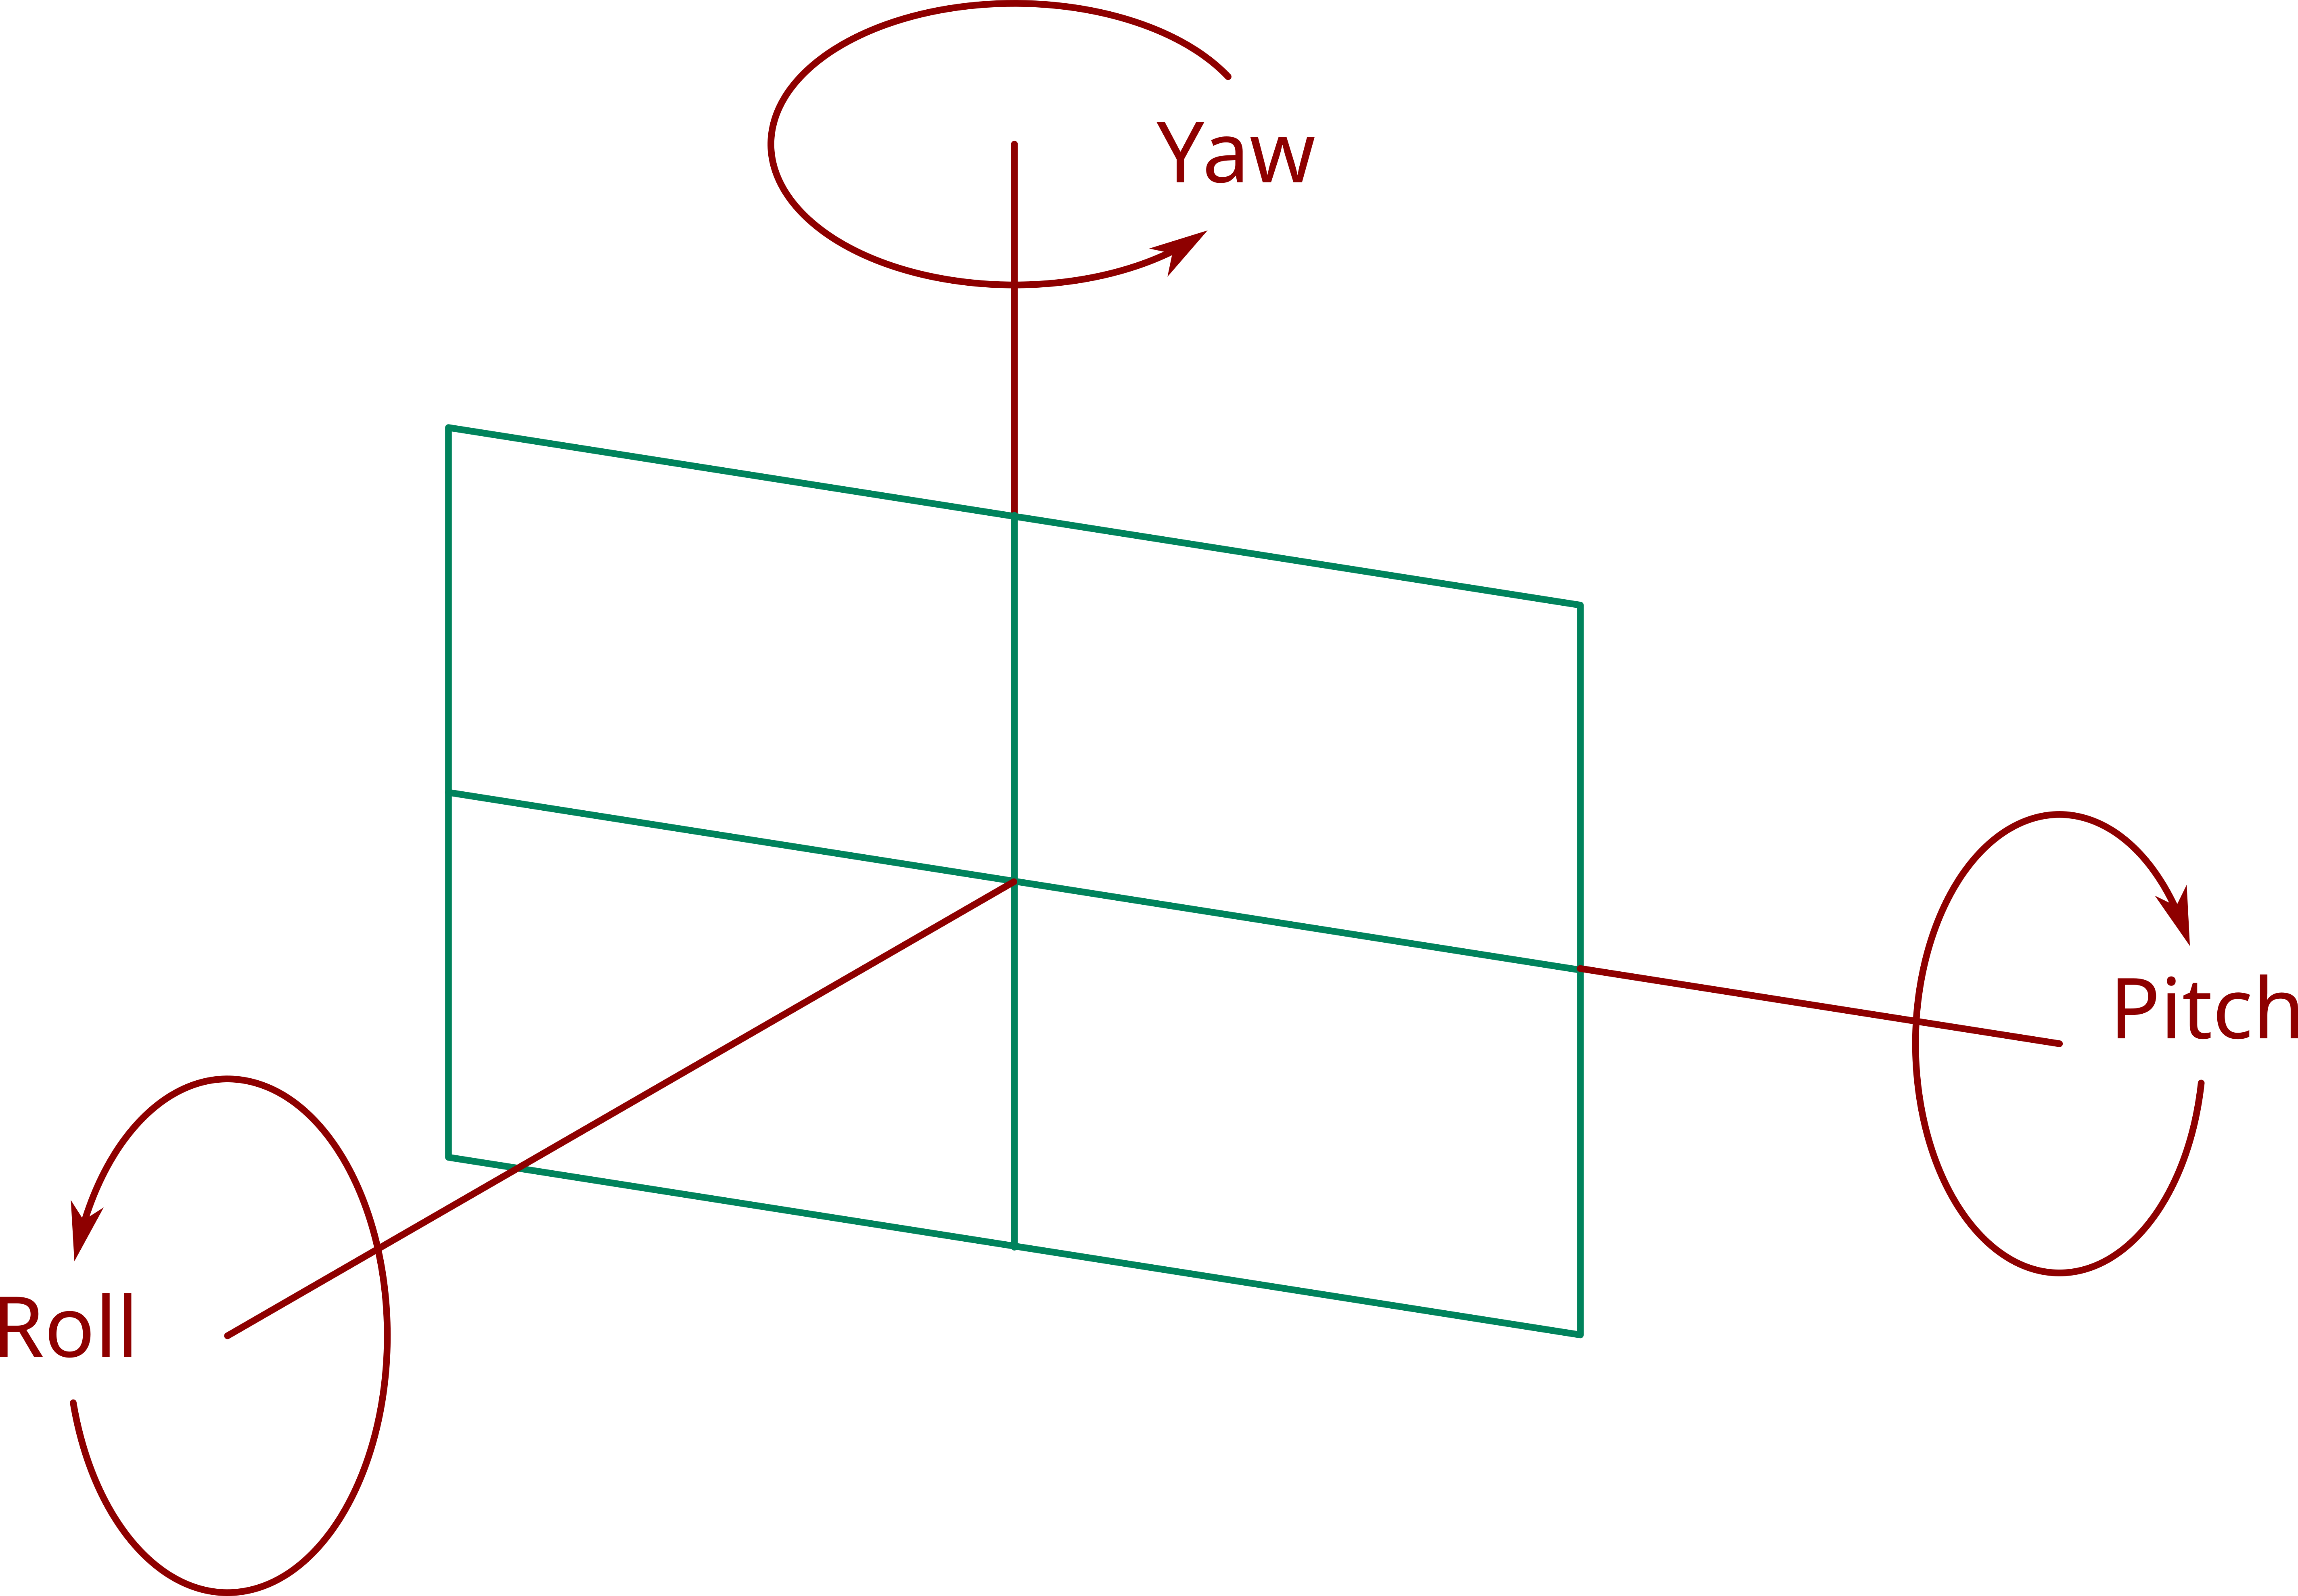
\includegraphics[width=.8\linewidth]{gfx/rollpitchyaw.png}
	\caption[Pitch, roll and yaw angles]{Pitch, roll and yaw angles}
	\label{fig:pitchrollyaw}
\end{figure}

This model let us compute the direction of the incoming rays just by indexing the particular pixel they hit, obtaining a map
\begin{equation}
	\label{eq:pixelmap}
	(p_x, p_y) \xmapsto{\mathfrak{h}_2} (\vartheta_{cs}, \varphi_{cs}),
\end{equation}
where $(p_x, p_y)$ are the components of the pixel in a system of coordinates whose origin is placed at the top-left corner of the sensor.

By composing \autoref{eq:initmap} and \autoref{eq:pixelmap}, we define the map
\begin{equation}
	(p_x, p_y) \xmapsto{\mathfrak{h} = \mathfrak{h_1}\circ\mathfrak{h_2}} (\vartheta', \varphi'),
\end{equation}
that summarises all the work the algorithm does: from a pixel on the camera's reference frame, we compute the origin of the incoming ray that hit that pixel.

\subsection{Pixel to Ray Map}
\label{subcsec:pixeltoray}

Let us consider a pixel $P$ whose coordinates on the sensor's reference frame are, in physical units, $(p_x, p_y)$, as depicted in \autoref{fig:pinhole}.

\begin{figure}[bth]
	\myfloatalign
	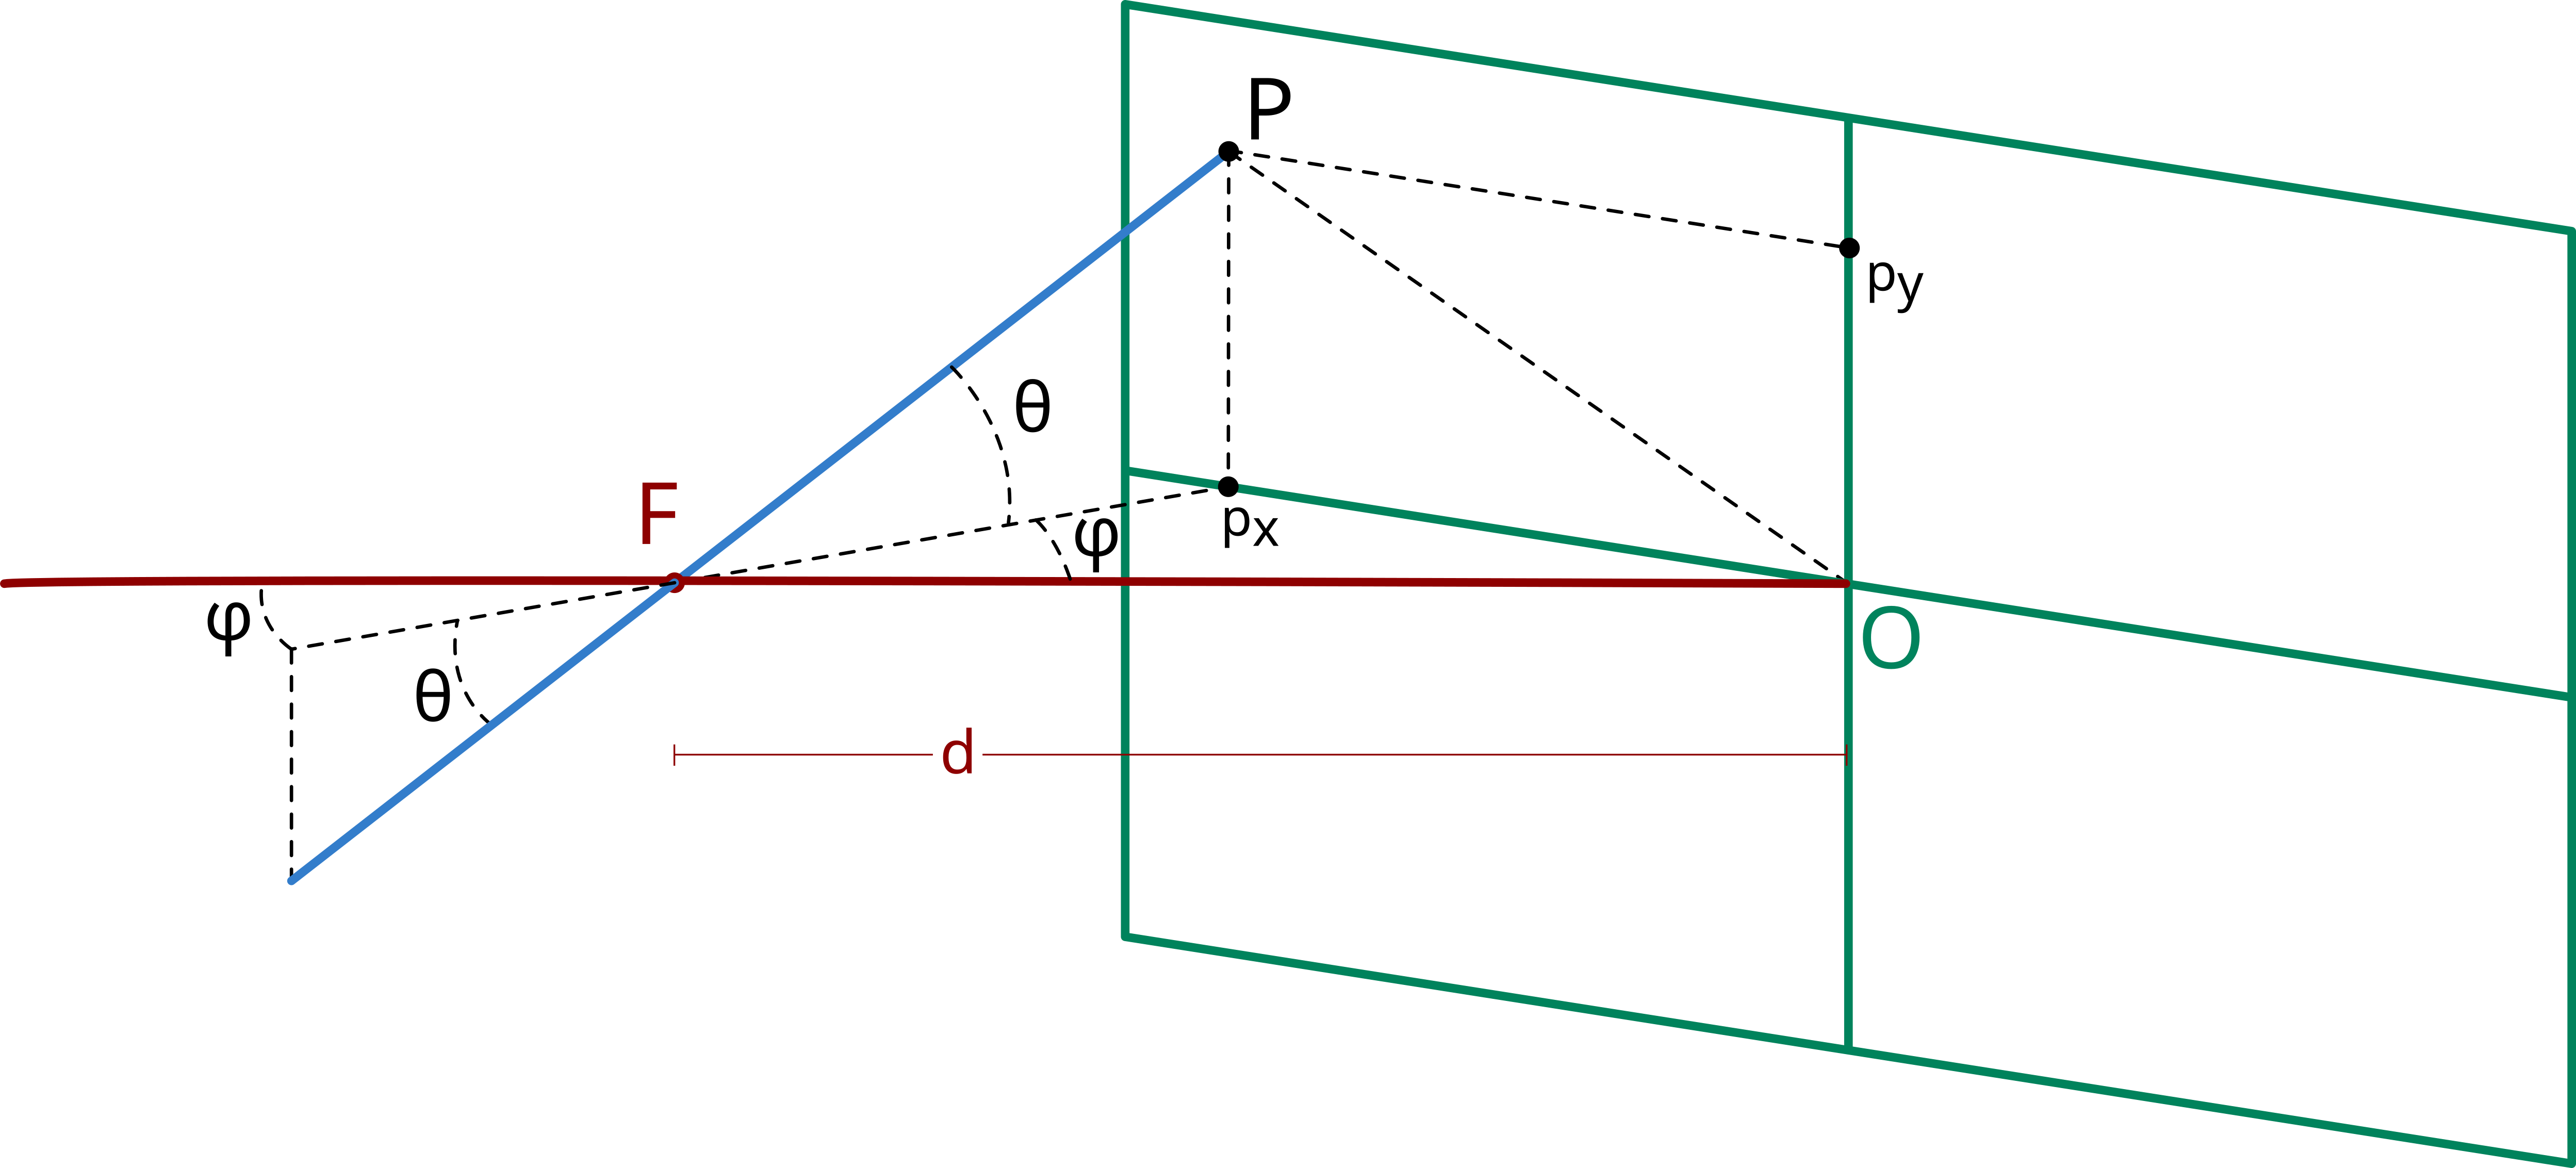
\includegraphics[width=.8\linewidth]{gfx/pinhole.png}
	\caption[Pinhole camera model]{Pinhole camera model}
	\label{fig:pinhole}
\end{figure}

All rays that hit the sensor are assumed, by our model, to pass through the focal point $F$. Thus, we can compute the angles $\vartheta$ and $\varphi$ for the ray hitting the sensor at pixel $P$ with elementary trigonometry.

From triangle $Fp_xO$ in \autoref{fig:pinhole}, we can obtain the angle $\varphi$ as
\[
	\varphi = \arctan{\frac{p_x}{d}}.
\]

Similary, the value of $\vartheta$ comes from the triangle $Fp_xP$ in \autoref{fig:pinhole}, which results in the following formula:
\[
	\vartheta = \arctan{\frac{p_y}{\sqrt{p_x^2 + d^2}}}.
\]

Finally, we need to adjust the zero for both $\vartheta$ and $\varphi$ to agree with the angle convention of the coordinate system. Therefore, the final formulas to computing the direction of an incoming ray hitting the camera's sensor ar a pixel $P = (p_x, p_y)$ are the following:
\begin{align}
	\vartheta_{cs} &= \frac{\pi}{2} + \arctan{\frac{p_y}{\sqrt{p_x^2 + d^2}}}, \\
	\varphi_{cs} &= \pi + \arctan{\frac{p_x}{d}}.
\end{align}

This discussion assumed the pixel coordinates to have its origin at the centre of the sensor. This is not the common coordinate system for pixels, as it usually have its origin at the top-left corner. A simple translation fixes that.

Furthermore, the pitch, roll and yaw angles were assumed to be zero. However, the addition of these angles is not difficult:
\begin{itemize}
	\item The roll angle, noted as $\alpha$, defines the rotation of the sensor on the image plane, so every pixel $(p_x, p_y)$ has to be rotated accordingly:
	\[
		\begin{pmatrix}
			p'_x \\
			p'_y
		\end{pmatrix} = 
		\begin{pmatrix}
			\cos\alpha & -\sin\alpha \\
			\sin\alpha & \cos\alpha 
		\end{pmatrix}
		\begin{pmatrix}
			p_x \\
			p_y
		\end{pmatrix}
	\]
	\item The pitch angle, noted as $\eta$, has to be simply added to the $\vartheta$ coordinate, as it defines the rotation of the sensor on that axis.
	\item The yaw angle, noted as $\lambda$, is the rotation of the sensor with respect to the $\varphi$ axis, so it has to be added to that coordinate.	
\end{itemize}

Taking all this into account, the final formulas to compute $(\vartheta_{cs}, \varphi_{cs})$ from the physical coordinates of the pixel $(p_x, p_y)$ are
\begin{align}
	\vartheta_{cs} &= \eta + \frac{\pi}{2} + \arctan{\frac{p_y}{\sqrt{p_x^2 + d^2}}}, \\
	\varphi_{cs} &= \lambda + \pi + \arctan{\frac{p_x}{d}}.,
\end{align}
where
\[
	p'_x = p_x\cos\alpha - p_y\sin\alpha, \qquad
	p'_y = p_x\sin\alpha + p_y\cos\alpha.
\]

\section{Initial Conditions Computation}
\label{sec:initcond}
The algorithm kernel integrates, backwards in time, an \ac{ODE} system. We already know the system we are working with, \autoref{theo:eqsmotion}, but for such a system to be uniquely solved, a set of initial conditions is needed.

That is, for each ray we need to know its components, \[(r, \vartheta, \varphi, p_r, p_\vartheta),\] at the time $\tau = 0$.

All rays hitting the camera share the same $r$, namely the position of the camera $r_c$.

In \autoref{subcsec:pixeltoray}, the initial $\vartheta_{cs}$ and $\varphi_{cs}$ for each ray were computed.

Therefore, we only need to compute the initial momentum components, $p_r$ and $p_\vartheta$, for each ray. In short, assuming we know the pixel the incoming ray is hitting and, thus, the $\vartheta_{cs}$ and $\varphi_{cs}$ components of the ray on the camera's local sky, we expect to obtain the map
\[
	(\vartheta_{cs}, \varphi_{cs}) \xmapsto{IC} (p_r, p_\vartheta).
\]

This is not a difficult task but a very delicate one, as some coordinate systems have to be taken into account and we should have a good understanding of them in order to properly compute the bases changes. A short summary of the work that follows is listed here:
\begin{enumerate}
	\item The initial position of the ray is known to be $(r_c, \vartheta_{cs}, \varphi_{cs})$. The components of the unit vector that points on the direction of motion of the camera, $B$, are noted as $(B_{\widehat{r}}, B_{\widehat{\vartheta}}, B_{\widehat{\varphi}})$, whereas its speed relative to the \ac{FIDO}, that is, the modulus of $B$, is noted as $\beta$.
	\item From $(\vartheta_{cs}, \varphi_{cs})$ we compute the unit vector in Cartesian coordinates, $N = (N_x, N_y, N_z)$, pointing to the direction of the incoming ray. This is computed on the camera's reference frame $\{e_x, e_y, e_z\}$, thus a simple change to Cartesian coordinates is needed.
	\item The relativistic aberration caused by the motion of the camera and its speed around the black hole causes the \ac{FIDO} to measure the direction of motion of the incoming ray slightly different. The Cartesian components of this derived unit vector, $n_F = (n_{F_x}, n_{F_y}, n_{F_z})$ need to be computed.
	\item Then, $n_F$ needs to be seen from the \ac{FIDO}'s orthonormal basis by means of the ligatures provided by the vector $B$ and the orthogonal relations. This gives us the components $(n_{F_{\widehat{r}}}, n_{F{\widehat{\vartheta}}}, n_{F_{\widehat{\varphi}}})$ on the basis $\{e_{\widehat{r}}, e_{\widehat{\vartheta}}, e_{\widehat{\varphi}}\}$.
	\item From $n_F$ expressed on the right coordinate system, we need to compute the covariant components of the four momentum $(p_t, p_r, p_\vartheta, p_\varphi)$, where we assume the energy to be unitary; \ie, $p_t = -E = -1$.
\end{enumerate}

\fixme{Explain more!}

\section{Numerical Solver}

Once we have the \ac{ODE} system and the initial conditions for the ray we want to solve, the final step is to numerically integrate, backwards in time, the geodesic followed by the ray.

The problem reduces then to numerically integrate an \ac{ODE} system, which is a well-known problem and widely studied in the literature.

In order to accomplish this task, the algorithm used by our ray tracer uses a classic Runge-Kutta method, along with an automated step size computation based on the estimated error of the step.

The Runge-Kutta method is based on the \texttt{DOPRI5} algorithm, described in \cite{hairer93} and \cite{hairer96}.

The automated control for the step size based on the estimated error follows the ideas in \cite[Sec. II.4, Subsec. Automatic Step Size Control]{hairer93}.

Furthermore, the step size is stabilized using the algorithm described in \cite[Sec. IV.2]{hairer96}.

\subsection{Adaptive Runge-Kutta Method}

The Runge-Kutta methods solve general initial values problems like the following one,
\begin{align*}
	\dot{y} = f(t,y) \\
	y(t_0) = y_0,
\end{align*}
where $y$ can be scalar or vector and $f$, $t_0$ and $y_0$ are known.

Given a pair $(t_n, y_n)$, the adaptive Runge-Kutta methods compute the value of the system at time $t_{n+1}$ as follows:
\begin{align*}
	y_{n+1} = y_n + h \sum_{i=1}^s b_i k_i\\
	y^*_{n+1} = y_n + h \sum_{i=1}^s b^*_i k_i,
\end{align*}

where $y_{n+1}$ is the new estimated value and $y^*_{n+1}$ is a higher order approximation that is used to estimate the error of the result, which is computed as $\vert y^*_{n+1} - y_{n+1} \vert$. In this notation, $h$ is the so-called \emph{step}, which is the amount of time the system is advanced, and the components $k_i$ are defined as follows:
\[
	k_i = f(t_n + c_ih, y_n + h\sum_{j=1}^{i-1} a_{ij} k_j).
\]

The coefficients $a_{ij}$, $b_i$, $b_i^*$ and $c_i$ define the model, and are usually arranged on what is called a Butcher's table (see \autoref{tab:generalbutcher} for a generic example).

\begin{table}[bth]
	\myfloatalign
	\begin{tabularx}{.54\textwidth}{c|ccccc}
		$0$&  & & & & \\
		$c_2$& $a_{21}$ & & & & \\
		$c_3$& $a_{31}$ & $a_{32}$ & & & \\
		$\vdots$& $\vdots$ &  & $\ddots$ & & \\
		$c_s$& $a_{s1}$  & $a_{s2}$ & $\cdots$ & $a_{s(s-1)}$ & \\ \hline
		& $b_1$ & $b_2$ & $\cdots$ & $b_{s-1}$ & $b_s$ \\ \hline
		& $b^*_1$ & $b^*_2$ & $\cdots$ & $b^*_{s-1}$ & $b^*_s$ \\
	\end{tabularx}
	\caption{Butcher's table for a generic adaptive Runge-Kutta method}
	\label{tab:generalbutcher}
\end{table}

Our system of \ac{ODE}, \autoref{theo:eqsmotion}, follows this model:
\begin{enumerate}
	\item $\dot{y} = (\dot{r}, \dot{\vartheta}, \dot{\varphi}, \dot{p}_r, \dot{p}_\vartheta)$,
	\item $f(t,y)$ is the right hand side of the equations and actually it does not depend on $t$, thus it can be written as $f(y)$.
	\item $t_0 = 0$ and $y_0 = (r_c, \vartheta_{cs}, \varphi_{cs}, p_{r}, p_{\vartheta})$ are the initial conditions computed in \autoref{sec:initcond}.
\end{enumerate}

The selected Runge-Kutta algorithm is a fourth order method with an estimation of the error based on a fifth order approximation, and whose Butcher's table is described on \autoref{tab:butcher}.

\begin{table}[bth]
	\myfloatalign
	\begin{tabularx}{.9\textwidth}{c|ccccccc}
		$0$&  & & & & & & \\
		$\frac{1}{5}$&  $\frac{1}{5}$& & & & & & \\
		$\frac{3}{10}$&  $\frac{3}{40}$&  $\frac{9}{40}$& & & & & \\
		$\frac{4}{5}$&  $\frac{44}{45}$&  $-\frac{56}{15}$&  $\frac{32}{9}$& & & & \\
		$\frac{8}{9}$&  $\frac{19372}{6561}$&  $-\frac{25360}{2187}$&  $\frac{64448}{6561}$&  $-\frac{212}{729}$& & & \\
		$1$&  $\frac{9017}{3168}$&  $-\frac{355}{33}$&  $\frac{46732}{5247}$&  $\frac{49}{176}$&  $-\frac{5103}{18656}$& & \\
		$1$&  $\frac{35}{384}$&  $0$&  $\frac{500}{1113}$&  $\frac{125}{192}$&  $-\frac{2187}{6784}$&  $\frac{11}{84}$& \\ \hline
		$y_1$&  $\frac{35}{384}$&  $0$&  $\frac{500}{1113}$&  $\frac{125}{192}$&  $-\frac{2187}{6784}$&  $\frac{11}{84}$&  $0$ \\ \hline
		$\widehat{y}_1$&  $\frac{5179}{57600}$&  $0$&  $\frac{7571}{16695}$&  $\frac{393}{640}$&  $-\frac{92097}{339200}$&  $\frac{187}{2100}$&  $\frac{1}{40}$
	\end{tabularx}
	\caption{Butcher's table for the ray tracer solver}
	\label{tab:butcher}
\end{table}

\subsection{Stabilization algorithm}

\section{Parallelization Techniques}

In general, the ray tracers are highly parallelizable, as they perform the same operations on different data.

In particular, our general relativity ray tracer is not different: it performs

\subsection{Classic Parallelization}
\subsection{General-Purpose Computing on Graphics Processing Units}
    \chapter{Solution Implementation}
\label{chapter:implementation}

This chapter covers the implementation details, the technologies used, the different decisions made and the reasons that led us to make them.

In short, the software developed is a Python package that implements a general relativity ray tracer using the library \ac{CUDA} as the back-end, generating images of a Kerr black hole from close distances.

The primary requirement when designing and implementing the software has been the \emph{ease of use}. The Python package exposes a minimal yet powerful public \ac{API}, abstracting all \ac{CUDA}-related code and letting the user configure the properties of the black hole and the cameras placed near it.

\section{Technologies Used}

The base code, exposed to the final user and with an easy to understand \ac{API}, is written in Python. The reason to choose this language is that it is widely used in the scientific community, and whose rise on these fields is increasing. Furthermore, it let us write simple understandable code withouth losing the power of the \ac{OOP}.

The \ac{CUDA} code is written in \ac{CUDA}-C, an extension of the well-known C language that permits to manage the \ac{GPU} and to establish a communication between the host (the \ac{CPU}) and the device (the \ac{GPU}). This is the most difficult code, highly optimised and where the ray tracer kernel and \ac{RK} solver are implemented.

In order to glue together the Python package and the \ac{CUDA} kernel, the PyCUDA library is used.

Finally, Sphinx has been used to manage the documentation of the package, letting the user access the Python docstrings on the objects defined. The C code has been documented using Doxygen, whose output is takes as an input by Sphinx in order to generate a complete documentation.

\subsection{Python Package}

The Python package is organised in four main files:
\begin{enumerate}
	\item \lstinline{universe.py}: defines a \lstinline{Universe} class, and exposes an instance of it to the package. This instace, called \lstinline{universe}, has all the general information about the spacetime, namely the black hole's spin and the accretion disk radius.
	\item \lstinline{camera.py}: defines a \lstinline{Camera} class, that contains all the necessary information that characterise it: the sensor size in physical units, the sensor resolution, the roll, pitch and yaw angles and its position with respect to the black hole centre. Internally, the \lstinline{Camera} class has an attribute called \lstinline{engine}, which is an instance of the \lstinline{RayTracer} class. The \lstinline{Camera} class is in charge of computing the $\alpha$, $\omega$ and $\varpi$ quantities, that defines the value of the Kerr metric on the point where the camera is placed.
	\item \lstinline{raytracer.py}: defines a \lstinline{RayTracer} class, which implements the PyCUDA calls to the \ac{CUDA} kernels. From the user perspective, it is the class that solves the \ac{ODE} system, although it delegates this work on the \ac{CUDA} methods.
	\item \lstinline{geodesics.py}: defines a main \lstinline{Congruence} class, which is a set of solved geodesics with their position at every computed time. There are two more classes defined in this file: \lstinline{GeodesicSnapshot}, which is a slice of the \lstinline{Congruence} containing the position of all computed geodesics at a single instant and \lstinline{Geodesic}, which is a slice of \lstinline{Congruence} containing one single geodesic with its position at all computed times.
\end{enumerate}

The workflow when using this package as a user would be: import the \lstinline{universe} instance and the \lstinline{Camera} class from the package, define as much cameras as desired and configure their properties, configure the spin of the black hole and the accretion disk through the \lstinline{universe} instance if the default values are not wanted and call the method \lstinline{shoot()} from an instance of the camera. This returns a \lstinline{CongruenceSnapshot} instance that can be plotted with its method \lstinline{plot()}.

\subsection{CUDA}

All \ac{CUDA} related files are stored in a directory inside the package. There are four main files inside that directory:
\begin{enumerate}
	\item \lstinline{raytracer.cu}: defines two kernels, \lstinline{setInitialConditions} and \lstinline{kernel}. They are explained with detail in \autoref{sec:cuda}.
	\item \lstinline{solvers.cu}: implements the \ac{RK} solver along with the automatic step size computation algorithm.
	\item \lstinline{image_transformation.cu}: defines a third kernel, \lstinline{generate_image}, that manages the texture maps. See \autoref{sec:cuda} for more details.
	\item \lstinline{functions.cu}: implements the right hand side of the \ac{ODE} system; \ie, the $f(y)$ function.
\end{enumerate}

\subsection{PyCUDA}

The interface between Python and \ac{CUDA} is implemented in the Python class \lstinline{RayTracer}. This class uses the PyCUDA module to configure the device, to manage the memory transactions between host and device and to execute the kernels on the device when the user on the host requests it.

\subsection{Documentation: Sphinx and Doxygen}

The documentation of the software has been made with Sphinx on the Python code and with Doxygen in the C code.

This let us set up a workflow where we document the objects and methods and then we generate different outputs. For example, Sphinx can render HTML documents, and a web page was designed in order to publish a good documentation that can be consulted from everywhere. This web page is not finished, and it is not included in the final code, but \autoref{fig:screenshot} shows an example screenshot of what it looks like.

\begin{figure}[bth]
	\myfloatalign
	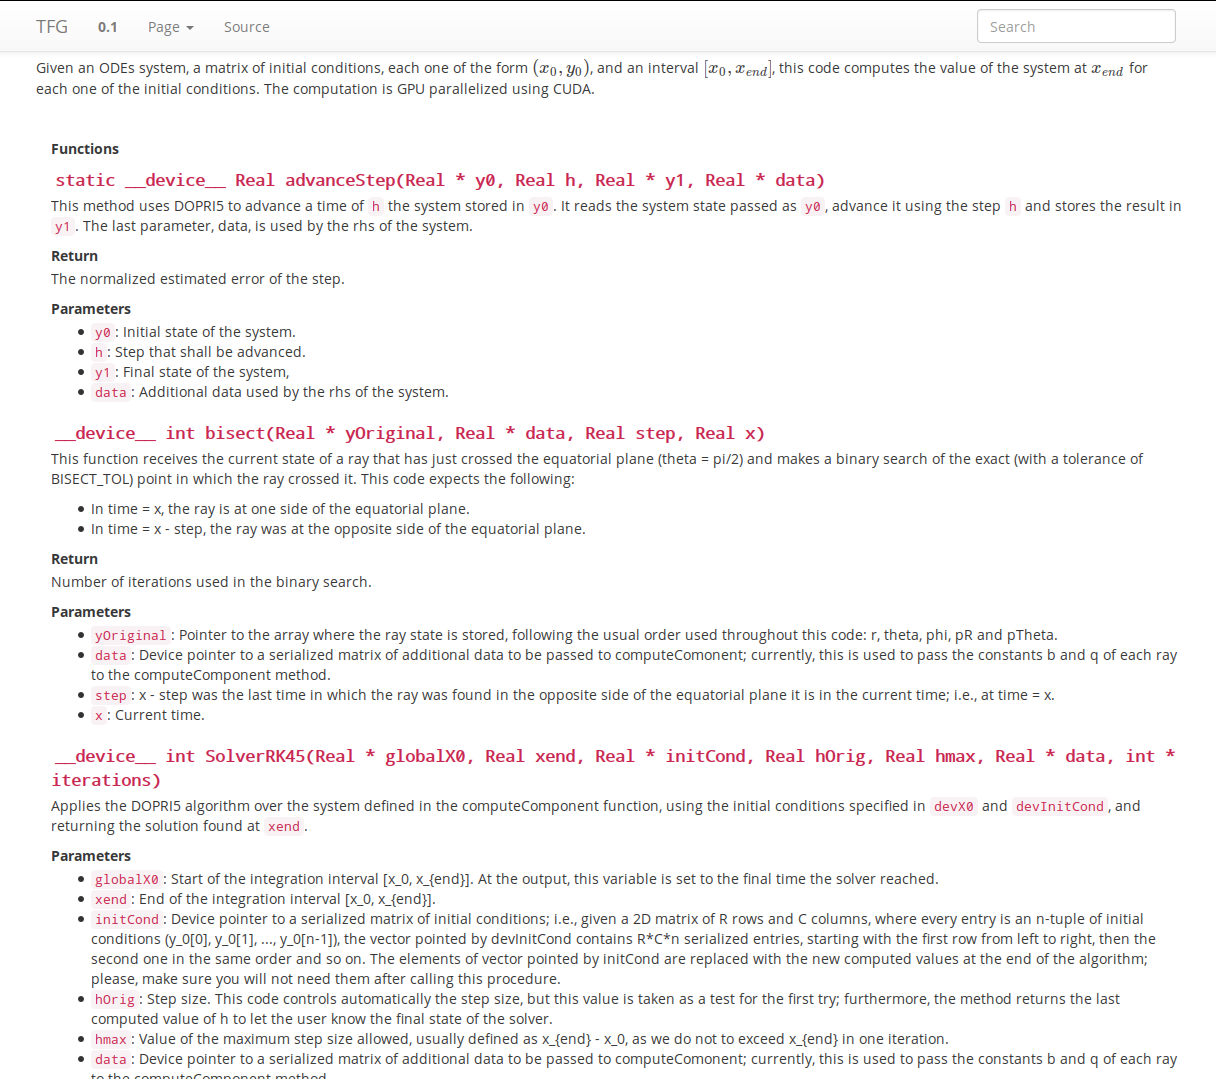
\includegraphics[width=\linewidth]{gfx/documentationscreenshot}
	\caption[Screenshot of the still unfinished web page]{Screenshot of the still unfinished web page.}
	\label{fig:screenshot}
\end{figure}

\section{Algorithm Implementation}

This section covers the implementation details for some of the most complex blocks on the code.

\section{CUDA Parallelization}
\label{sec:cuda}

\ac{CUDA} is a powerful library that abstracts the interaction with the \ac{GPU} in order to let the user implement general purpose programs on it.

\ac{CUDA} abstracts all kinds of \acp{GPU} in a hierarchy to manage instructions and shared memory. A list with the main levels on the hierarchy follows:
\begin{itemize}
	\item \emph{Thread}: the minimal unit managed by the \ac{GPU}. It is a set of data and instructions that is handled by a single processing unit of the \ac{GPU}. It has its own local memory, the fastest of all the memories defined by \ac{CUDA}, and is only accessible by the thread itself.
	\item \emph{Warp}: a logical set of 32 threads that execute the same instruction at the same time on different data. Although the consideration of the warps can be omitted by developers, a good design that takes this into account can increase the performance highly, as a warp takes advantage of the spatial locality of data, optimising accesses to memory.
	\item \emph{Block}: a three dimensional (although one can omit any of the dimensions) matrix where every element is a thread. All threads in a block can access a section of the memory, called \emph{shared memory}, which is much faster than the global memory. Every thread has a unique per-block identifier.
	\item \emph{Grid}: a three dimensional (although one can omit any of the dimensions) matrix where every element is a block. The memory accessible by all threads in all blocks is called the \emph{global memory}, and it is the slowest one. Every block has a unique identifier within the grid.
\end{itemize}

The \ac{CUDA} device is configured once at the beginning of the program as a set of threads, uniquely identified by their block indices and thread indices relative to the blocks.

\begin{figure}[bth]
	\myfloatalign
	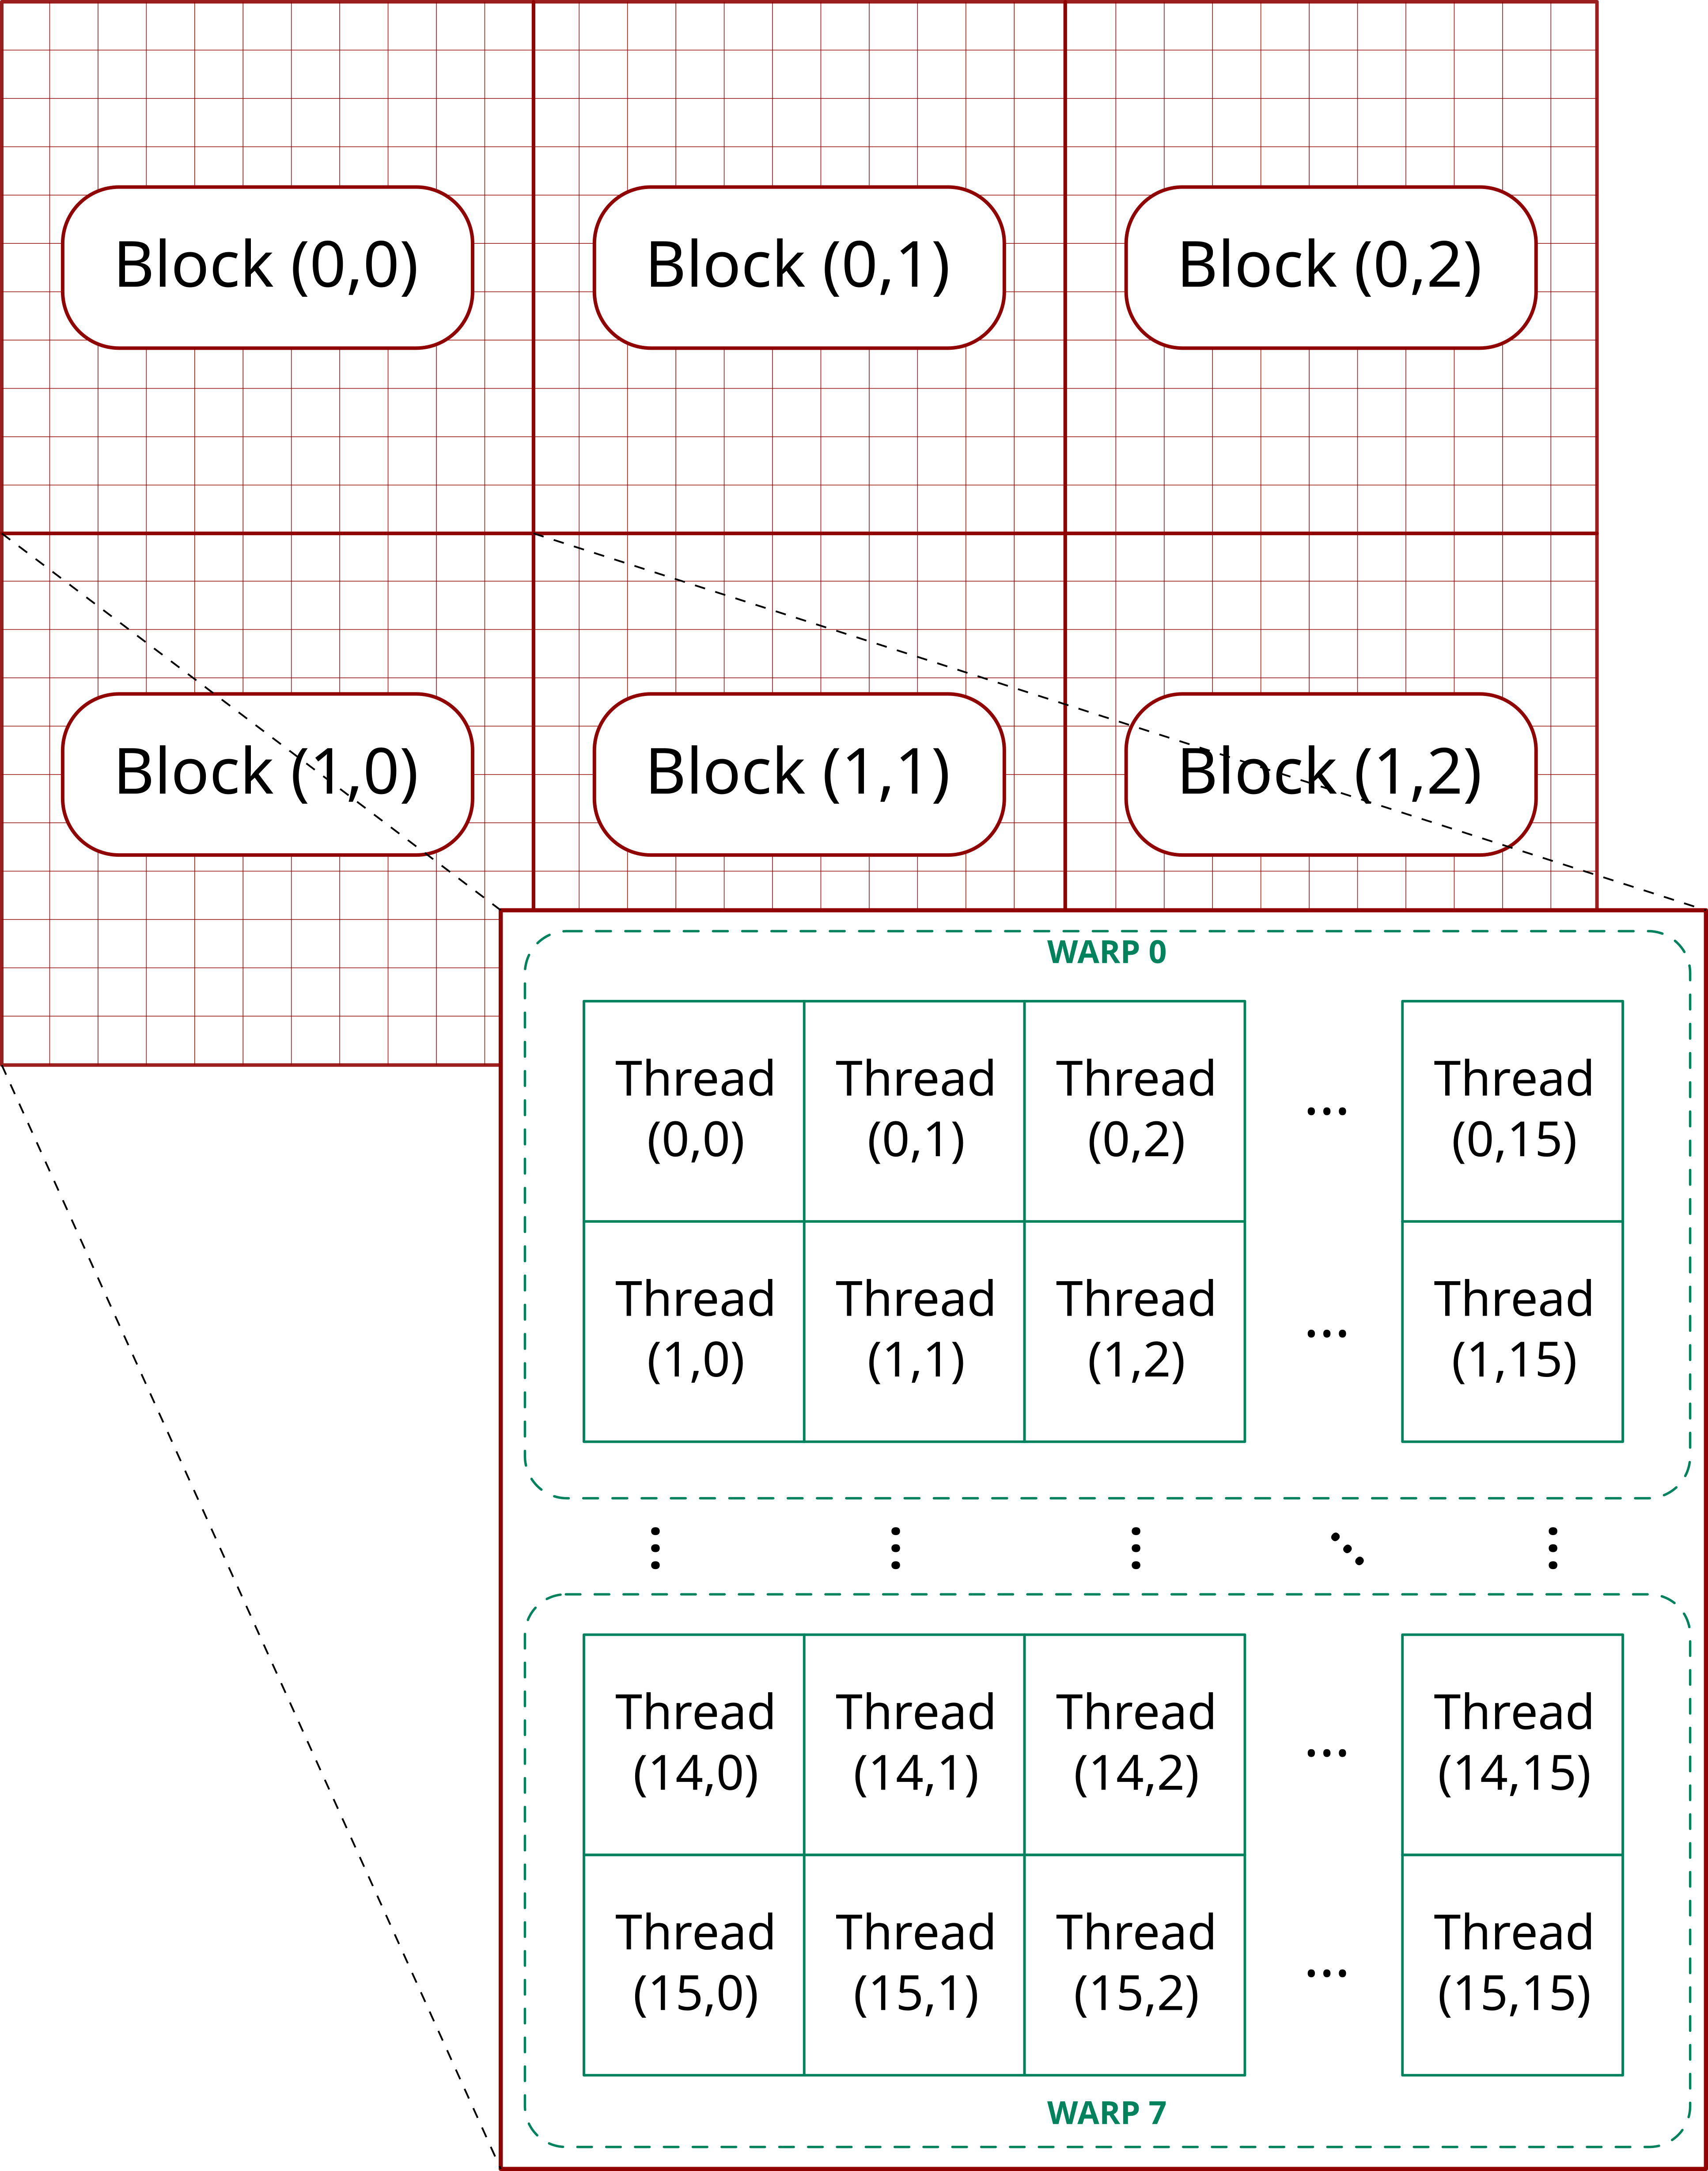
\includegraphics[width=.8\linewidth]{gfx/cudagrid}
	\caption[$2\times3$ grid with $16\times16$ blocks]{$2\times3$ grid with $16\times16$ blocks}
	\label{fig:cudagrid}
\end{figure}

An example configuration of the \ac{CUDA} device can be seen on \autoref{fig:cudagrid}, where 6 two dimensional blocks are arranged on the grid in two rows and three columns. Every block has 256 threads, arranged on a 16$\times$16 matrix.

The shape of the \ac{CUDA} grid and blocks are customizable by the user, but the warps are automatically created by \ac{CUDA}, picking up always sets of successive 32 threads, going first through the $X$ axis, then through the $Y$ axis and finally through the $Z$ axis.

This section will study how the grid and blocks are shaped on our software and the implemented parallelized code, as well as some fine-tuning techniques used to speed up the computations.

\subsection{Device Setup}

The configuration of the grid for a ray tracer seems natural. As we are working with images, which are simply two dimensional matrices, the grid will be shaped as a two dimensional matrix, where every thread will compute the geodesic corresponding to a pixel.

The important question now is how to configure the pixels between the blocks; \ie, how to define the number of blocks per column and per row in the grid.

The simplest answer is to define one dimensional blocks of a fixed size that extend along the rows of the image. The very first implementation of the ray tracer used this configuration, but the speed up against the \ac{CPU} implementation was very poor.

The branch divergence was guilty of the poor performance: along a row of the image, the behaviour of the corresponding geodesics is very different, and the so-called \emph{warp divergence} occurs: in a warp, which in this configuration is defined along the rows of the image, all threads execute the same instruction at the same time; if the control flow varies between the threads in a warp, some of them will be idle, which causes a great loss of parallel efficiency.

This is avoided by designing a configuration that ensures, or at least that facilitates, that all the threads in a warp execute the same exact code without branch divergence. In our case, this means that the geodesics hitting the pixels in a warp should have followed a nearby path.

However, without knowing a priori the origin of the geodesics, we can only guess which pixels will have similar geodesics. The configuration design follows then this sensible guess: \emph{nearby pixels are hit by geodesics with nearby origins}.

From this assumption, we designed warps as squared as possible, configuring the blocks to have an integer number of warps. This resulted in the following configuration:
\begin{enumerate}
	\item Each block has $8\times8$ threads; \ie, two warps of $8\times4$ threads are located per block. See \autoref{fig:warpconf}.
	\begin{figure}[bth]
		\myfloatalign
		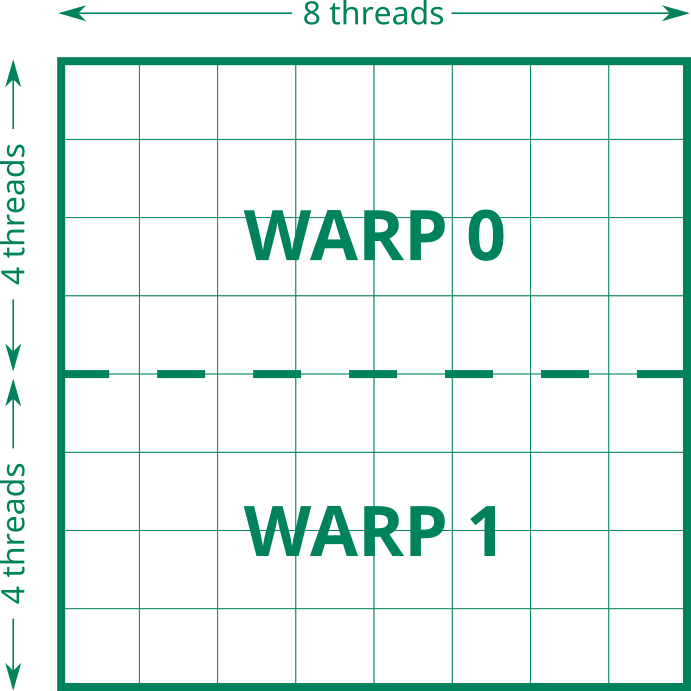
\includegraphics[width=.5\linewidth]{gfx/warpconf.png}
		\caption[Raytracer block configuration]{Raytracer block configuration}
		\label{fig:warpconf}
	\end{figure}
	\item The grid size is dynamically computed using the image size provided by the user. The number of rows and columns of the grid are computed with the following formulas:
	\begin{equation*}
	G_C = \left \lfloor{\frac{I_C - 1}{B_C} + 1}\right \rfloor, \qquad
	G_R = \left \lfloor{\frac{I_R - 1}{B_R} + 1}\right \rfloor,
	\end{equation*}
	where $G_C$ and $G_R$ are the number of blocks per column and per row, $I_C$ and $I_R$ are the columns and rows of pixels of the image and $B_C = B_R = 8$ are the number of columns and rows of a block. These formulas ensure we have enough threads to compute each pixel. The remaining threads, which do not have any geodesic to compute, will be idle during all the program execution.
\end{enumerate}

\subsection{CUDA Kernels}

The main function executed by \ac{CUDA} on the \ac{GPU} is called the \emph{kernel}. Our implementation has three kernels, where every thread is identified with a pixel via its unique identifier in the \ac{CUDA} device. The kernels are:
\begin{enumerate}
	\item \lstinline{setInitialConditions()}: it is the kernel to compute the initial conditions for every pixel, as designed in \autoref{sec:initcond}. From the pixel coordinates, it computes the corresponding pair $(\vartheta_{cs}, \varphi_{cs})$.
	\item  \lstinline{kernel()}: it is the main kernel. It receives the initial conditions for every pixel and the final time until which the \ac{ODE} system will be integrated. It computes the origin of each geodesic, \ie, the pair $(\vartheta', \varphi')$, using the design described at \autoref{sec:numerical}, while continuously checking for collisions with the accretion disk.
	\item \lstinline{generate_image()}: it is an auxiliary kernel to map textures into the images. It receives the origin of the geodesic corresponding to each pixel in the image and maps it to a pixel in the provided texture.
\end{enumerate}

\subsection{Optimizations}

The computational bottleneck of the ray tracer is the \ac{ODE} solver. In particular, the computation of the right hand side of the system ---in terms of the \autoref{sec:numerical}, the function $f(y,t)$---, which involves a lot of operations, some of them really expensive, as the \lstinline{sin()} and \lstinline{cos()} functions.

This chunk of code has been highly optimised, pre-computing all repeated operations and using efficient implementations such as the \lstinline{sincos()} function. The derivatives on equations \ref{eq:eqsmotionp}, \ref{eq:eqsmotionpr} and \ref{eq:eqsmotionpt} have been expressed in their most elementary terms and all common quantities between them have been also pre-computed. To optimise the memory access time, the thread's local memory has been used whenever it was possible.

Furthermore, a specific issue has been taking into account: the \ac{ILP}. It is clear that a single thread cannot keep the \ac{GPU} busy, so the device schedules threads and instructions in such a way that the \ac{GPU} is always busy.

One way of helping the \ac{CUDA} scheduler to maximize the device occupancy is to design the code optimising the \ac{ILP}. For example, imagine the following three lines of code:

\begin{lstlisting}
	int rho = a + b;
	int theta = c + d;
	int m = rho * theta;
\end{lstlisting}

It is clear that the third one depends on the other two to be executed. However, the first two lines can be run in parallel. The scheduler then can run these two operations on different processor in order to speed up the computation.

All the ray tracer implementation is coded in such a way that independent instructions are together, whereas dependent ones are as far as possible one of the other. This let the scheduler issue instructions in parallel without having to wait for dependent computations to finish.

In particular, the code of the computation of $f(y,t)$ has been deeply studied in order to maximize the \ac{ILP}.

\subsection{Initial Conditions Computation}

The initial conditions computation is implemented as a kernel on the \lstinline{raytracer.cu} file.

It receives a pointer to two allocated sections of memory in the device: one to store the output of the initial conditions and another to store the output of the computation of the conserved quantities $b$ and $q$.

Each thread solve the formulas obtained in \autoref{sec:pinhole}: equations \ref{eq:pinhole1} and \ref{eq:pinhole2} and the ones obtained in \autoref{sec:initcond}, and store the computed values in the pointed sections of the memory.

\subsection{Ray Tracing}

The ray tracing kernel implements the main logic of the software: it executes the \ac{RK} solver while continuously checking for collisions with either the disk or the black hole, following the design on \autoref{sec:numerical}.

It receives a pointer to an allocated section of the memory where the initial conditions of the system are stored. After solving the \ac{ODE} system, it rewrites this buffer to provide the user with the final \ac{BL} coordinates of the considered geodesics.

An auxiliary buffer is used in order to known if a given geodesic has hit the disk, has fallen into the black hole or if it points to the celestial sphere.

\subsection{Texture Mapping}

The texture mapping is a simple kernel implemented in the \lstinline{image_transformation.cu} file. It receives the final computed solution of the \ac{ODE} system, a pointer to a section of the memory where the textures pixels are assumed to be stored along with the size of the textures and a pointer to another previously allocated section of memory where the final pixels of the image will be stored.

It then computes the texture mapping and outputs the result to the final image.
    \chapter{Documentation Development}


    \chapter{Results}

\section{Computational results}


\subsection{Runge-Kutta Solver Accuracy}

\begin{figure}[bth]
	\myfloatalign
	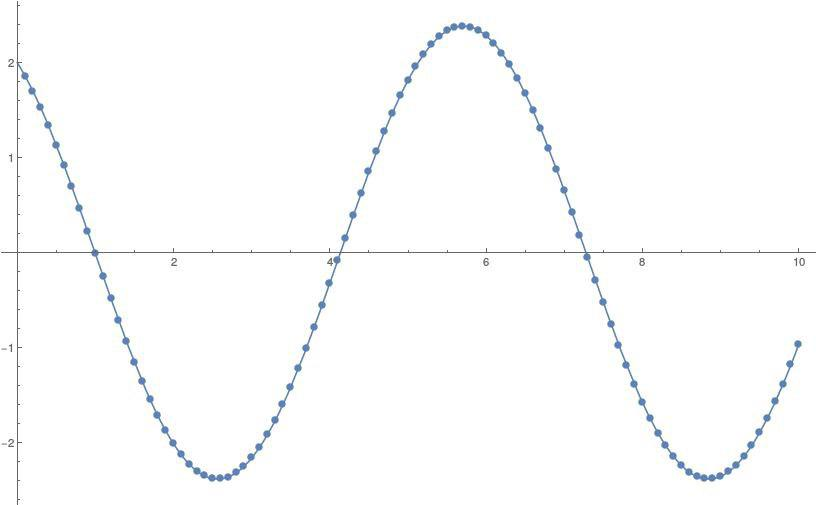
\includegraphics[width=.5\linewidth]{gfx/stepcomputation.jpg}
	\caption[Automatic step computation]{Automatic step computation}
	\label{fig:stepsize}
\end{figure}

\begin{figure}[bth]
	\myfloatalign
	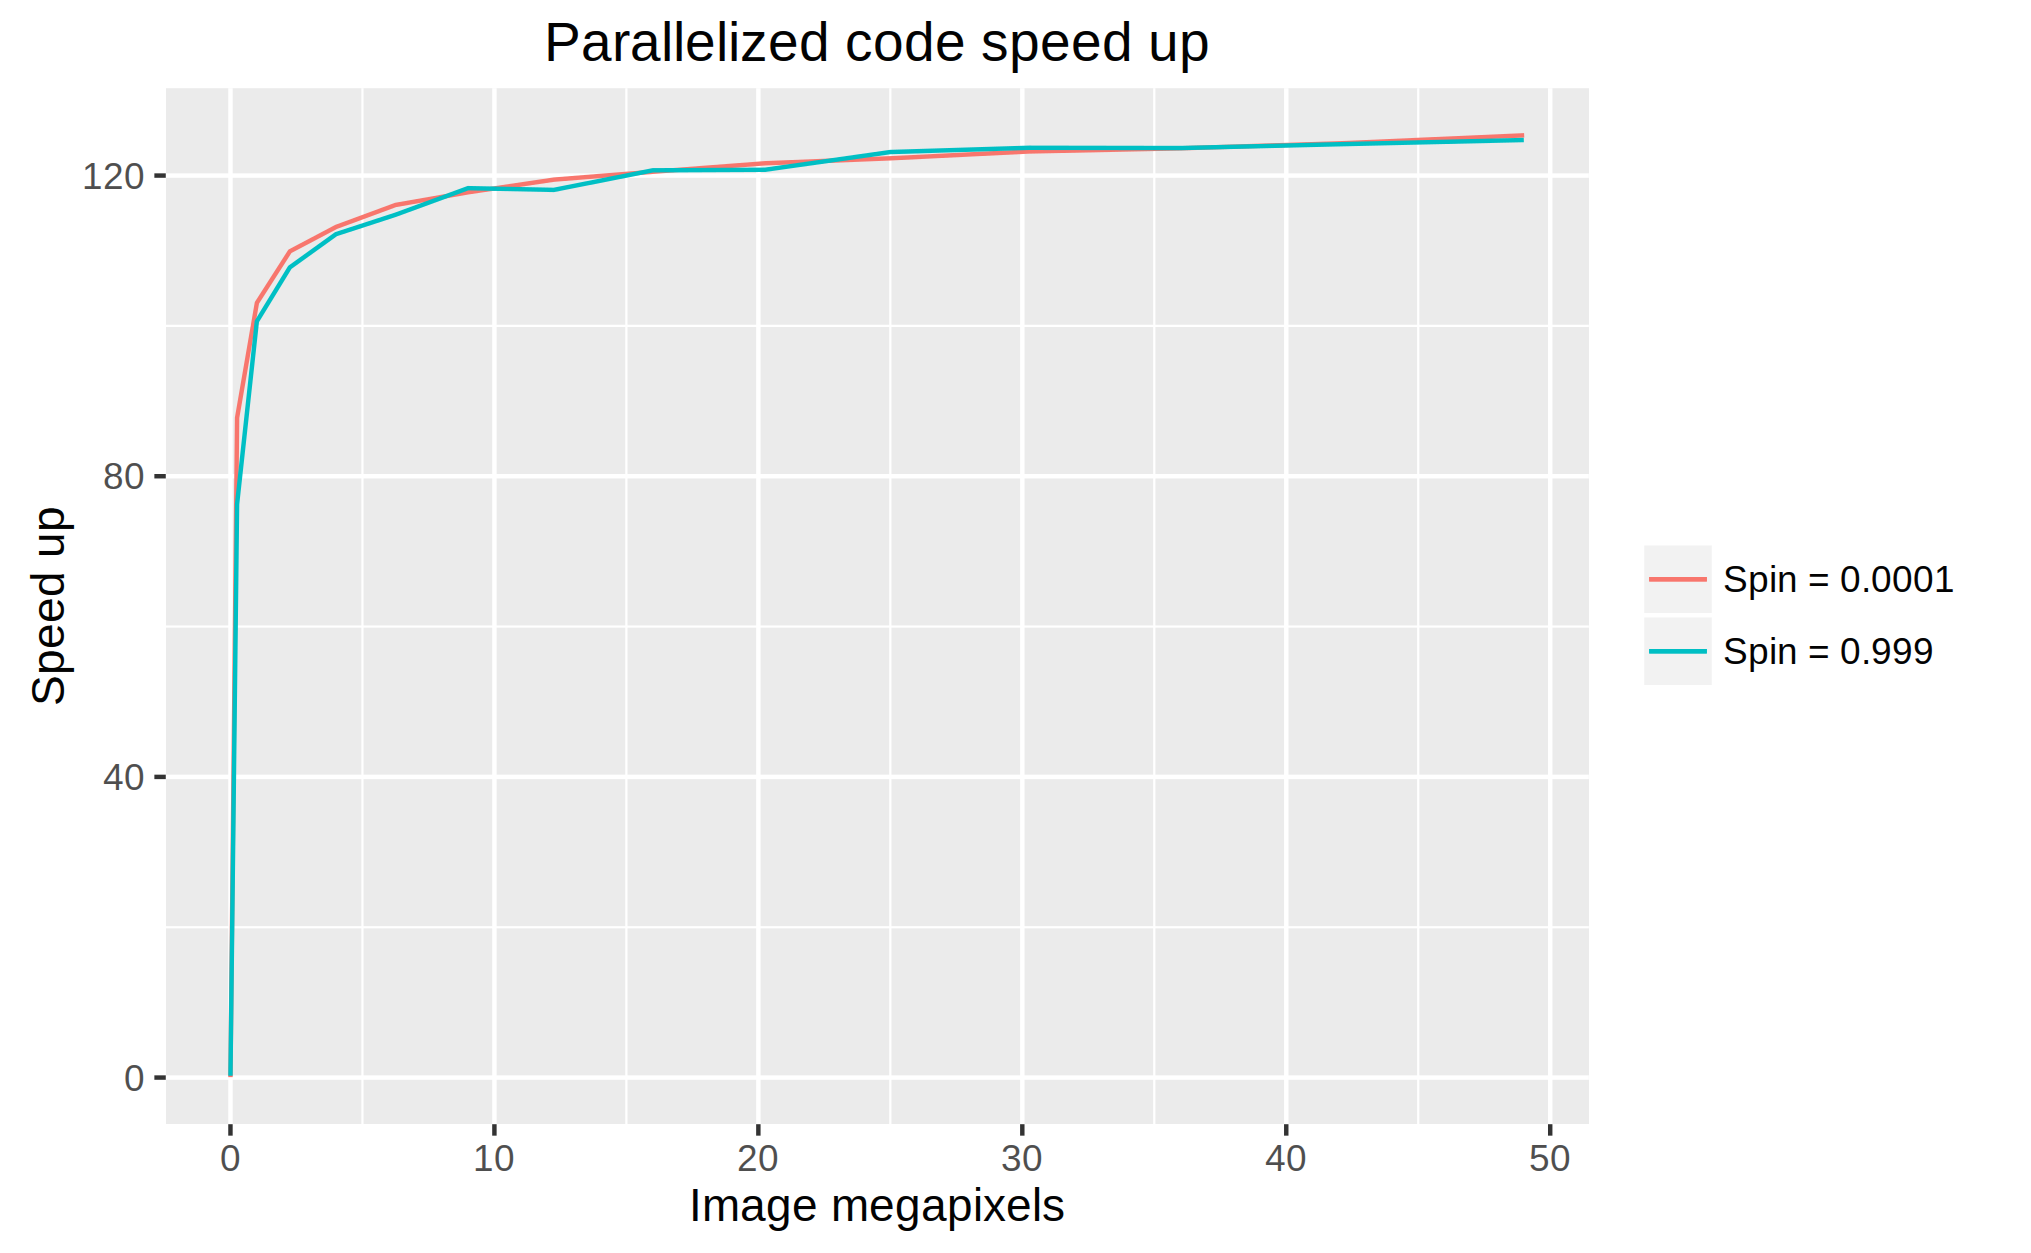
\includegraphics[width=\linewidth]{gfx/speedup.png}
	\caption[Speed up with different spins]{Speed up with different spins}
	\label{fig:speedup}
\end{figure}


\section{Scientific results}
    
    \part{Conclusions}

    \cleardoublepage

% ********************************************************************
% Backmatter
%*******************************************************
    %\appendix
    %\renewcommand{\thechapter}{\alph{chapter}}
    %\cleardoublepage
    %\part{Appendix}
    %\chapter{Killing vectors and Killing tensors}\label{Killingchapter}
To obtain a simple form of the geodesic equations of a spacetime, a useful tool are Killing vectors. In a simple way, the Killing vectors are objects that inform us of symmetries of the spacetime and its metric. Using their properties we can obtain first integrals of the geodesic equations. Therefore, understanding the Killing vectors of a space time is an important step to obtain more simple equations for the geodesic flow.

\section{Properties of Killing vectors}

Formally Killing vectors are defined as:
\begin{equation}
\mathcal{L}_\xi g = 0,
\end{equation}
where $\mathcal{L}_\xi$ is the Lie derivative along the vector field $\xi$. If the manifold has a torsion-free metric connection $\nabla$, this expression becomes:
\begin{align}\label{killingformula}
{L}_\xi g_{a b} &= \xi^c \nabla_c g_{a b} + g_{a c} \nabla_b \xi^c + g_{c b} \nabla_a \xi^c \\ \nonumber
&= \nabla_b \xi_a +  \nabla_a \xi_b = 0 ,
\end{align}
where $g_{\alpha \beta}$ is the spacetime metric and the indices will be raised and lowered with $g$.

\section{Killing vectors and Lagrangian symmetries}

We will see that Lagrangian symmetries correspond to the Killing vectors of the spacetime. For this purpose consider:
\begin{align}\label{lagrangianodeff}
&v \in T_p M \\
&L(v,p)= \frac{1}{2} g|_p (v|_p,v|_p)
\end{align}
Considering a generic vector $Y \in T_p M$, we will move $\mathcal{L}$ along the one-parameter group $\phi_t$ generated by $Y$. If we name $\phi_t$ the tangent aplication $\phi$ we will have that:
\begin{align}
Y(L(v|_p,p))&= \frac{d}{dt}|_{t=0} \left( L (\phi_{*_t}(v),\phi_t(p)) \right)  \\
&=\frac{d}{dt}|_{t=0} \left( \frac{1}{2} g|_{\phi_t(p)} (\phi_{*_t}(v),\phi_{*_t}(v)) \right) \label{Lagrangiansimetrie}
\end{align}
In geometric terms all you are doing is moving the vector $ v $ by the group of diffeomorphisms $\phi_t$ and contracting it with the metric evaluated at $\phi_t(p)$. This process is the same as applying the pull-back to the metric evaluated at $\phi_t(p)$ and contract it in $p$ with the vector being evaluated at $p$. That is, given $\omega \in T^*_pM$, $v \in T_pM$ and $\phi_t$ a diffeomorphism, they fulfill:
\begin{equation}
\phi_t^*(\omega|_{\phi_t(p)})|_p(v|_p)= \omega ( \phi_{*_t}(v|_p))|_{\phi_t(p)}
\end{equation}
Therefore, from \cref{Lagrangiansimetrie} it follows that:
\begin{align}
 & \frac{1}{2} \frac{d}{dt}|_{t=0} \phi^*_t(g|_{\phi_t(p)})|_p (v|_p,v|_p) \\
 &=-\frac{1}{2} \lim_{t \to 0} \frac{ \phi^*_0(g|_{\phi_t(p)}) - \phi^*_t(g|_{\phi_t(p)})|_p }{t}(v|_p,v|_p) =-\frac{1}{2} \mathcal{L}_Y(g)(v|_p,v|_p)
\end{align}
If $\mathcal{L}_Y(g)=0$ then $Y$ is a Killing field and is also a symmetry of the Lagrangian.

\section{Killing vectors and first integrals}

Killing vectors are useful among many other reasons for defining conserved quantities. The definition of the conserved quantities is simply the dot product of the Killing vector for the tangent vector of the geodesic:
\begin{align}
 u^\beta \nabla_\beta (\xi_\alpha u^\alpha)&= u^\beta \xi_\alpha \nabla_\beta  u^\alpha+ u^\beta u^\alpha \nabla_\beta \xi_\alpha  \\
&= u^\beta u^\alpha \nabla_\beta \xi_\alpha  = u^\alpha u^\beta \nabla_\beta  \xi_\alpha  \\ &= \frac{1}{2} \left( u^\alpha u^\beta \nabla_\beta \xi_\alpha  + u^\alpha u^\beta \nabla_\alpha \xi_\beta  \right) = 0 \label{killingintegrals}
\end{align}
and hence we obtain that, along the geodesic:
\begin{equation}\label{killingconstants}
g(u,\xi) = cte
\end{equation}

\section{Noether currents and Killing vectors}

It is convenient to relate the Noether currents defining the symmetries of a Lagrangian and the Killing vectors of the metric. Noether currents of a Lagrangian satisfied that:
\begin{equation}
\dot{q^\alpha} \nabla_\alpha J + \ddot{q^\alpha} \nabla_\alpha J= 0
\end{equation}
where $q^\alpha$ and $ \dot{q}^\alpha$ are the are natual coordinates on the tangent bundle $J$ is defined, in case that the Lagrangian remains invariant under a symmetry generated by $\xi$, as:
\begin{equation}
J = \frac{\partial \mathcal{L}}{\partial (\dot{q^\alpha})} \xi^\alpha
\end{equation}
At infinitesimal level, the transformation whose generator is $ \xi $ takes the form:
\begin{equation}
q^\alpha \to q^\alpha + \xi^\alpha
\end{equation}
In the case of the Lagrangian  of \cref{lagrangianodeff}:
\begin{align}
J &= \frac{\partial \frac{1}{2} g_{\alpha \beta} \dot{q^{\alpha}} \dot{q^{\beta}} }{\partial (\dot{q^\gamma})} \xi^\gamma =\frac{1}{2} (g_{\gamma \beta} \dot{q^{\beta}} + g_{\alpha \gamma} \dot{q^{\alpha}}) \xi^\gamma \\ &= g_{\gamma \beta} \dot{q^{\beta}} \xi^\gamma =g(\dot{q},\xi)
\end{align}
And we get that for Killing vectors, the Noether currents are exactly the conserved geometric quantities associated Killing vector $\xi$.

\section{Killing Tensors}
A generalization of the Killing vector equation can be achieved generalizing the \cref{killingformula} for tensors:
\begin{equation}
\nabla_{(\alpha} T_{\beta \gamma )} = 0
\end{equation}
Thus, the following conserved quantities (using \cref{killingintegrals} ) will hold:
\begin{equation}
T_{\alpha \beta} u^\alpha u^\beta = cte
\end{equation}
There are Killing tensors that comes from tensor products of Killing vectors, and therefore does not provide independent conserved quantities. In other words, the Killing tensors:
\begin{equation}
T_{i j} = \xi_i \otimes \xi_j
\end{equation}
generate the conserved quantities:
\begin{align}
T_{i j} u^i u^j = c_i c_j
\end{align}
where $c_i=g(u,\xi_i)$.
\section{Killing algebra}
An useful property is that, given two Killing vectors $\xi_1$ y $\xi_2$:
\begin{equation}
\xi_3=[\xi_1,\xi_2]
\end{equation}
Is also a Killing vector because:
\begin{equation}
\mathcal{L}_{[\xi_1,\xi_2]} g=[\mathcal{L}_{\xi_1} ,\mathcal{L}_{\xi_2} ]g= 0
\end{equation} 
It is well-known that the set of all the complete vector fields on a manifold constitute also a Lie algebra which is naturally identifiable to the Lie algebra of the isometry group of the (semi-Riemannian) manifold.  When completeness is dropped, analogous considerations hold locally.

%********************************************************************
% Other Stuff in the Back
%*******************************************************

   \cleardoublepage% Change name from Bibliography to References
\renewcommand\bibname{References}
\renewcommand\contentsname{References}

%********************************************************************
% Bibliography
%*******************************************************
% work-around to have small caps also here in the headline
\manualmark
\markboth{\spacedlowsmallcaps{\bibname}}{\spacedlowsmallcaps{\bibname}} % work-around to have small caps also
%\phantomsection
\refstepcounter{dummy}
\addtocontents{toc}{\protect\vspace{\beforebibskip}} % to have the bib a bit from the rest in the toc
\addcontentsline{toc}{chapter}{\tocEntry{\bibname}}
\label{app:bibliography}
\nocite{*}

% \printbibliography
   \cleardoublepage%*******************************************************
% Declaration
%*******************************************************
\refstepcounter{dummy}
\pdfbookmark[0]{Declaration}{declaration}
\chapter*{Declaration}
\thispagestyle{empty}
Put your declaration here.
\bigskip
 
\noindent\textit{\myLocation, \myTime}

\smallskip

\begin{flushright}
    \begin{tabular}{m{5cm}}
        \\ \hline
        \centering\myName \\
    \end{tabular}
\end{flushright}

   \cleardoublepage\pagestyle{empty}

\hfill

\vfill


\pdfbookmark[0]{Colophon}{colophon}
\section*{Colophon}
This document was typeset using the typographical look-and-feel \texttt{classicthesis} developed by Andr\'e Miede. 
The style was inspired by Robert Bringhurst's seminal book on typography ``\emph{The Elements of Typographic Style}''. 
\texttt{classicthesis} is available for both \LaTeX\ and \mLyX: 
\begin{center}
\url{https://bitbucket.org/amiede/classicthesis/}
\end{center}
Happy users of \texttt{classicthesis} usually send a real postcard to the author, a collection of postcards received so far is featured here: 
\begin{center}
\url{http://postcards.miede.de/}
\end{center}
 
\bigskip

\noindent\finalVersionString

%Hermann Zapf's \emph{Palatino} and \emph{Euler} type faces (Type~1 PostScript fonts \emph{URW
%Palladio L} and \emph{FPL}) are used. The ``typewriter'' text is typeset in \emph{Bera Mono}, 
%originally developed by Bitstream, Inc. as ``Bitstream Vera''. (Type~1 PostScript fonts were made 
%available by Malte Rosenau and
%Ulrich Dirr.)

%\paragraph{note:} The custom size of the textblock was calculated
%using the directions given by Mr. Bringhurst (pages 26--29 and
%175/176). 10~pt Palatino needs  133.21~pt for the string
%``abcdefghijklmnopqrstuvwxyz''. This yields a good line length between
%24--26~pc (288--312~pt). Using a ``\emph{double square textblock}''
%with a 1:2 ratio this results in a textblock of 312:624~pt (which
%includes the headline in this design). A good alternative would be the
%``\emph{golden section textblock}'' with a ratio of 1:1.62, here
%312:505.44~pt. For comparison, \texttt{DIV9} of the \texttt{typearea}
%package results in a line length of 389~pt (32.4~pc), which is by far
%too long. However, this information will only be of interest for
%hardcore pseudo-typographers like me.%
%
%To make your own calculations, use the following commands and look up
%the corresponding lengths in the book:
%\begin{verbatim}
%    \settowidth{\abcd}{abcdefghijklmnopqrstuvwxyz}
%    \the\abcd\ % prints the value of the length
%\end{verbatim}
%Please see the file \texttt{classicthesis.sty} for some precalculated 
%values for Palatino and Minion.
%
%    \settowidth{\abcd}{abcdefghijklmnopqrstuvwxyz}
%    \the\abcd\ % prints the value of the length






% ********************************************************************
% Game Over: Restore, Restart, or Quit?
%*******************************************************
    \end{document}

% ********************************************************************
